\documentclass[11pt]{article}
\usepackage{cmap}
\usepackage[T1]{fontenc}
\usepackage[utf8]{inputenc}
\usepackage[sc]{mathpazo}
\linespread{1.05}
\usepackage[a4paper,margin=26mm]{geometry}
\usepackage{amsmath,amssymb,amsthm,mathtools,booktabs,array,longtable,graphicx,xcolor,enumitem,microtype}
\usepackage[hidelinks,pdftitle={Universal Rank-Three Obstructions in Binary Arithmetic Occurrence Geometry: Circuit Decomposition Rigidity, Vector-Space Partitions, and Universal Non-Embedding Theorems},pdfauthor={UNNS Research Collective}]{hyperref}
\newcommand{\geoicommit}{\texttt{343f9aef\allowbreak 2b669746\allowbreak 6058165c\allowbreak 5fc2ddf0\allowbreak f00e882b}}
\usepackage[capitalise,noabbrev]{cleveref}
\usepackage{caption}
\captionsetup{font=small,labelfont=bf}
\setlist{itemsep=2pt,topsep=3pt}
\setlength{\emergencystretch}{3em}

\newtheorem{theorem}{Theorem}[section]
\newtheorem{lemma}[theorem]{Lemma}
\newtheorem{proposition}[theorem]{Proposition}
\newtheorem{corollary}[theorem]{Corollary}
\theoremstyle{definition}
\newtheorem{definition}[theorem]{Definition}
\newtheorem{example}[theorem]{Example}
\theoremstyle{remark}
\newtheorem{remark}[theorem]{Remark}
\newtheorem{question}{Question}

% ---- notation ----
\newcommand{\F}{\mathbb F}
\newcommand{\Z}{\mathbb Z}
\newcommand{\R}{\mathbb R}
\newcommand{\Q}{\mathbb Q}
\newcommand{\one}{\mathbf 1}
\newcommand{\supp}{\operatorname{supp}}
\newcommand{\wt}{\operatorname{wt}}
\newcommand{\spn}{\operatorname{span}}
\newcommand{\rk}{\operatorname{rank}}
\newcommand{\Circ}{\mathcal C}
\newcommand{\Part}{\Pi}
\newcommand{\relint}{\operatorname{relint}}
\newcommand{\AG}{\mathrm{AG}}
\newcommand{\AGL}{\mathrm{AGL}}
\newcommand{\GL}{\mathrm{GL}}
\newcommand{\rmin}{r_{\min}}
\newcommand{\conf}{\sqsubseteq}
\newcommand{\sgn}{\operatorname{sgn}}
\newcommand{\src}[1]{\par\smallskip\noindent{\footnotesize\textit{Source status.} #1\par}\smallskip}
\newcommand{\gid}[1]{\texttt{#1}}
\newcommand{\figdesc}[1]{\textit{Description:} #1}
\newcommand{\PROVED}{\textsc{proved}}
\newcommand{\CHECKED}{\textsc{checked}}
\crefname{theorem}{Theorem}{Theorems}
\crefname{lemma}{Lemma}{Lemmas}
\crefname{proposition}{Proposition}{Propositions}
\crefname{corollary}{Corollary}{Corollaries}
\crefname{definition}{Definition}{Definitions}
\crefname{example}{Example}{Examples}
\crefname{remark}{Remark}{Remarks}

\title{Universal Rank-Three Obstructions in Binary Arithmetic Occurrence Geometry\\[2pt]
\large Circuit Decomposition Rigidity, Vector-Space Partitions,\\ and Universal Non-Embedding Theorems}
\author{UNNS Research Collective\thanks{UNNS Substrate Research Program, \texttt{unns.tech}. GEO-I Manuscript~II.}}
\date{28 October 2026}

\newcommand{\classtablebody}{$3$ & $4$ & $3$ & $2^{3}$ & $1$ & $24$\\
$4$ & $6$ & $4$ & $2^{4},\,3^{1}$ & $28$ & $48$\\
$4$ & $7$ & $7$ & $2^{7}$ & $8$ & $168$\\
$4$ & $8$ & $7$ & $2^{7}$ & $1$ & $1344$\\
$5$ & $8$ & $8$ & $2^{8},\,4^{1}$ & $840$ & $384$\\
$5$ & $9$ & $9$ & $2^{9},\,3^{2}$ & $4480$ & $72$\\
$5$ & $10$ & $12$ & $2^{12},\,3^{1}$ & $6720$ & $48$\\
$5$ & $10$ & $15$ & $2^{15}$ & $448$ & $720$\\
$5$ & $11$ & $12$ & $2^{12},\,3^{1}$ & $1680$ & $192$\\
$5$ & $11$ & $15$ & $2^{15}$ & $2688$ & $120$\\
$5$ & $12$ & $12$ & $2^{12},\,3^{1}$ & $140$ & $2304$\\
$5$ & $12$ & $15$ & $2^{15}$ & $1680$ & $192$\\
$5$ & $13$ & $15$ & $2^{15}$ & $560$ & $576$\\
$5$ & $14$ & $15$ & $2^{15}$ & $120$ & $2688$\\
$5$ & $15$ & $15$ & $2^{15}$ & $16$ & $20160$\\
$5$ & $16$ & $15$ & $2^{15}$ & $1$ & $322560$\\}
\newcommand{\ksixtablebody}{$10$ & $1$ & $16$ & $16$\\
$12$ & $2$ & $16$ & $21$\\
$13$ & $4$ & $22$ & $25$\\
$14$ & $10$ & $22$ & $31$\\
$15$ & $15$ & $24$ & $31$\\
$16$ & $25$ & $24$ & $31$\\
$17$ & $23$ & $25$ & $31$\\
$18$ & $26$ & $25$ & $31$\\
$19$ & $22$ & $28$ & $31$\\
$20$ & $22$ & $28$ & $31$\\
$21$ & $16$ & $28$ & $31$\\
$22$ & $15$ & $28$ & $31$\\
$23$ & $9$ & $28$ & $31$\\
$24$ & $8$ & $28$ & $31$\\
$25$ & $5$ & $31$ & $31$\\
$26$ & $4$ & $31$ & $31$\\
$27$ & $2$ & $31$ & $31$\\
$28$ & $2$ & $31$ & $31$\\
$29$ & $1$ & $31$ & $31$\\
$30$ & $1$ & $31$ & $31$\\
$31$ & $1$ & $31$ & $31$\\
$32$ & $1$ & $31$ & $31$\\}
\newcommand{\ksixtotal}{215}
\newcommand{\smallptablebody}{$4$ & $3$ & $1$ & $1$ & $1$ & $3$\\
$5$ & $3$ & $0$ & $0$ & $0$ & ---\\
$5$ & $4$ & $4$ & $4$ & $0$ & ---\\
$6$ & $3$ & $0$ & $0$ & $0$ & ---\\
$6$ & $4$ & $6$ & $6$ & $6$ & $4$\\
$6$ & $5$ & $11$ & $11$ & $0$ & ---\\
$7$ & $3$ & $0$ & $0$ & $0$ & ---\\
$7$ & $4$ & $4$ & $4$ & $4$ & $7$\\
$7$ & $5$ & $55$ & $55$ & $0$ & ---\\
$7$ & $6$ & $26$ & $26$ & $0$ & ---\\
$8$ & $3$ & $0$ & $0$ & $0$ & ---\\
$8$ & $4$ & $1$ & $1$ & $1$ & $7$\\
$8$ & $5$ & $165$ & $165$ & $10$ & $8$\\
$8$ & $6$ & $325$ & $325$ & $0$ & ---\\
$8$ & $7$ & $57$ & $57$ & $0$ & ---\\}
\newcommand{\identitytablebody}{$3$ & $4$ & $2^{3}$ & $6=6$ & $0=0$\\
$4$ & $6$ & $2^{4},3^{1}$ & $14=14$ & $24=24$\\
$4$ & $7$ & $2^{7}$ & $14=14$ & $14=14$\\
$4$ & $8$ & $2^{7}$ & $14=14$ & $0=0$\\
$5$ & $8$ & $2^{8},4^{1}$ & $30=30$ & $128=128$\\
$5$ & $9$ & $2^{9},3^{2}$ & $30=30$ & $126=126$\\
$5$ & $10$ & $2^{12},3^{1}$ & $30=30$ & $120=120$\\
$5$ & $10$ & $2^{15}$ & $30=30$ & $120=120$\\
$5$ & $11$ & $2^{12},3^{1}$ & $30=30$ & $110=110$\\
$5$ & $11$ & $2^{15}$ & $30=30$ & $110=110$\\
$5$ & $12$ & $2^{12},3^{1}$ & $30=30$ & $96=96$\\
$5$ & $12$ & $2^{15}$ & $30=30$ & $96=96$\\
$5$ & $13$ & $2^{15}$ & $30=30$ & $78=78$\\
$5$ & $14$ & $2^{15}$ & $30=30$ & $56=56$\\
$5$ & $15$ & $2^{15}$ & $30=30$ & $30=30$\\
$5$ & $16$ & $2^{15}$ & $30=30$ & $0=0$\\}
\newcommand{\witnesstablebody}{$3$ & $4$ & $\{1,2\}\,|\,\{3,4\}$ & $\{1,3\}\,|\,\{2,4\}$ & $\{2,3\}$ & $3$\\
$4$ & $6$ & $\{1,3,5\}\,|\,\{2,4,6\}$ & $\{1,4,5\}\,|\,\{2,3,6\}$ & $\{1,2\}$ & $3$\\
$4$ & $7$ & $\{1,2,3,4\}\,|\,\{5,6,7\}$ & $\{1,4,5\}\,|\,\{2,3,6,7\}$ & $\{2,3,5\}$ & $3$\\
$4$ & $8$ & $\{1,2,3,4\}\,|\,\{5,6,7,8\}$ & $\{1,2,5,6\}\,|\,\{3,4,7,8\}$ & $\{3,4,5,6\}$ & $3$\\
$5$ & $8$ & $\{1,3,5,7\}\,|\,\{2,4,6,8\}$ & $\{1,4,5,7\}\,|\,\{2,3,6,8\}$ & $\{1,2\}$ & $3$\\
$5$ & $9$ & $\{1,5,6,7\}\,|\,\{2,3,4,8,9\}$ & $\{1,3,5,8\}\,|\,\{2,4,6,7,9\}$ & $\{1,2,3\}$ & $3$\\
$5$ & $10$ & $\{1,4,5,8\}\,|\,\{2,3,6,7,9,10\}$ & $\{1,4,6,7,8\}\,|\,\{2,3,5,9,10\}$ & $\{1,2,3,4\}$ & $3$\\
$5$ & $10$ & $\{1,2,3,4,5,6\}\,|\,\{7,8,9,10\}$ & $\{1,2,4,7\}\,|\,\{3,5,6,8,9,10\}$ & $\{3,5,6,7\}$ & $3$\\
$5$ & $11$ & $\{1,4,6,7,9\}\,|\,\{2,3,5,8,10,11\}$ & $\{1,4,5,8,9\}\,|\,\{2,3,6,7,10,11\}$ & $\{1,2,3,4\}$ & $3$\\
$5$ & $11$ & $\{1,2,3,4,5,6,7\}\,|\,\{8,9,10,11\}$ & $\{1,4,6,7,8\}\,|\,\{2,3,5,9,10,11\}$ & $\{2,3,5,8\}$ & $3$\\
$5$ & $12$ & $\{1,2,5,6,9,10\}\,|\,\{3,4,7,8,11,12\}$ & $\{1,2,7,8,9,10\}\,|\,\{3,4,5,6,11,12\}$ & $\{1,2,3,4\}$ & $3$\\
$5$ & $12$ & $\{1,2,3,4,5,6,7,8\}\,|\,\{9,10,11,12\}$ & $\{1,4,6,7,9\}\,|\,\{2,3,5,8,10,11,12\}$ & $\{2,3,5,8,9\}$ & $3$\\
$5$ & $13$ & $\{1,2,3,4,5,6,7,8\}\,|\,\{9,10,11,12,13\}$ & $\{1,2,7,8,9,10\}\,|\,\{3,4,5,6,11,12,13\}$ & $\{3,4,5,6,9,10\}$ & $3$\\
$5$ & $14$ & $\{1,2,3,4,5,6,7,8\}\,|\,\{9,10,11,12,13,14\}$ & $\{1,2,7,8,9,10\}\,|\,\{3,4,5,6,11,12,13,14\}$ & $\{3,4,5,6,9,10\}$ & $3$\\
$5$ & $15$ & $\{1,2,3,4,5,6,7,8\}\,|\,\{9,10,11,12,13,14,15\}$ & $\{1,2,3,4,9,10,11,12\}\,|\,\{5,6,7,8,13,14,15\}$ & $\{5,6,7,8,9,10,11,12\}$ & $3$\\
$5$ & $16$ & $\{1,2,3,4,5,6,7,8\}\,|\,\{9,10,11,12,13,14,15,16\}$ & $\{1,2,3,4,9,10,11,12\}\,|\,\{5,6,7,8,13,14,15,16\}$ & $\{5,6,7,8,9,10,11,12\}$ & $3$\\}
\newcommand{\typestablebody}{$3$ & $[1^{3}]$ & $1$\\
$4$ & $[1^{7}]$ & $2$\\
$4$ & $[1^{4}\,2^{1}]$ & $1$\\
$5$ & $[1^{15}]$ & $7$\\
$5$ & $[1^{12}\,2^{1}]$ & $3$\\
$5$ & $[1^{8}\,3^{1}]$ & $1$\\
$5$ & $[1^{9}\,2^{2}]$ & $1$\\
$6$ & $[1^{31}]$ & $134$\\
$6$ & $[1^{28}\,2^{1}]$ & $59$\\
$6$ & $[1^{25}\,2^{2}]$ & $12$\\
$6$ & $[1^{24}\,3^{1}]$ & $4$\\
$6$ & $[1^{22}\,2^{3}]$ & $3$\\
$6$ & $[1^{16}\,2^{5}]$ & $1$\\
$6$ & $[1^{16}\,4^{1}]$ & $1$\\
$6$ & $[1^{21}\,2^{1}\,3^{1}]$ & $1$\\}

\begin{document}
\maketitle

\begin{abstract}
\noindent Let $M$ be a binary matrix with columns $c_1,\dots,c_n$ and $C=\ker M\subseteq\F_2^n$ its code. The nonzero codewords, read as $0/1$ vectors, are the integer points of the box $[0,1]^n$ in the lattice $\Lambda_M=\{\alpha\in\Z^n: M\alpha\equiv 0 \bmod 2\}$. Conformally minimal (Graver) lattice vectors with corners in this fibre span parallelepipeds, the \emph{cells}. The box is \emph{embedded} if the cells meet face to face and \emph{non-embedded} otherwise; a non-embedded box contains a \emph{collision} of two cells with intersecting relative interiors, and its \emph{minimum witness rank} $\rmin$ is the least dimension of the affine span of a collision.

We prove, from the definitions and without recourse to any computation in the central steps: (i) a box is non-embedded if and only if some codeword has two distinct decompositions into disjoint circuits (minimal supports); (ii) in a coordinatewise-minimal non-embedded box the all-ones word lies in $C$, all other words have a unique circuit decomposition, and the reduced coordinate set is a spanning subset $X$ of an affine space $\AG(k-1,2)$ with $|X|=p\ge k+1$; (iii) the partitions of the all-ones word into circuits give a vector-space partition of $C/\langle\one\rangle\cong\F_2^{k-1}$, which satisfies an exact counting identity and a Parseval identity; (iv) these force at least $p-1$ two-circuit partitions of $\one$ when $p\ge 9$, sharp for $X=\AG(k-1,2)$; and, with a finite check for $p\le 8$, \emph{every} minimal non-embedded box has at least two such partitions; (v) consequently $\rmin=3$ for \emph{every} non-embedded box of the frozen binary model, and there is no minimal box with $\rmin\ge4$. We also give an explicit rank-three obstruction (the even-weight code of length~4), the complete classification of minimal reduced boxes for nullity $3,4,5$ (with $1,3,12$ classes; reproduced here by an independent exhaustive enumeration) and, as source-reported results with independently re-checked representatives, nullity $6$ ($215$ classes).

The scope is the frozen binary $0/1$ Graver-cell model. The results do not assert that every binary code is realized by a rational arithmetic occurrence fibre, and rank three is a statement about a local witness: it is not a polynomial-time algorithm for deciding embeddedness. Proof status, stated precisely: for $p\ge9$ reduced coordinates the universal statements (including $n_2\ge p-1$) are proved analytically in the text; the case $p\le8$ is closed by a complete, exhaustive finite enumeration (a computer-assisted step, with own code and exact arithmetic), so the universality of W2 and hence $\rmin=3$ rest on that enumeration together with the analytic argument. Classification counts for nullity $3,4,5$ are re-enumerated here; the nullity-$6$ list of $215$ classes is source-reported, its completeness is inherited from the release and no universal claim depends on it.
\end{abstract}

\medskip\noindent\textbf{Keywords:} binary linear codes, circuits, Graver basis, conformal minimality, vector-space partitions, finite affine geometry, non-embedding, Parseval identity.\\
\textbf{Mathematics Subject Classification (provisional, to be confirmed):} 94B05, 05B35, 51E20, 52B20, 11H06.

\tableofcontents
\clearpage

%% ===================================================================
%% PART I
%% ===================================================================
\part{Foundations}

%% -------------------------------------------------------------------
\section{Introduction: the geometry of non-embedding}\label{sec:intro}

\subsection{Relation to arithmetic occurrence geometry}\label{sec:aog}

This paper continues the study of \emph{arithmetic occurrence geometry}, a term defined in the companion planar manuscript \cite{PaperA} (in its Introduction and, formally, directly after the derivation of the occurrence fibre $F_x$ in its Section~2): the study of finite arithmetic occurrence fibres, their exact coordinate relationships, and explicitly specified geometric realizations constructed upon those relationships. The occurrence coordinates are determined by arithmetic; the cell constructions are separately specified structures, so that the intrinsic organization of the occurrences is distinguished from the properties of a particular realization. Whereas the companion manuscript investigates exceptional topology and convex stabilization for two active prime coordinates, the present paper addresses embedding obstructions in a specified higher-dimensional \emph{binary $0/1$ Graver-cell construction}.

\emph{Specialization.} In the notation of this paper, the arithmetic occurrence fibre is replaced by the fibre $F=C\setminus\{0\}$ of a binary code $C=\ker M$ (the nonzero $0/1$ points of the relation lattice $\Lambda_M$), and the realization is the Graver-cell construction of Section~\ref{sec:cells} restricted to the box $[0,1]^n$. Binary relation lattices form a mathematically tractable family in which circuit decompositions, cell collisions and minimum obstruction ranks can be investigated exactly. The conclusions concern this specified construction. They do not presume that every binary configuration is realized by a rational occurrence fibre (see also Section~\ref{sec:intro-scope}). We use \emph{arithmetic occurrence geometry} in the sense defined in the companion manuscript \cite{PaperA}: the study of distinct arithmetic occurrence fibres, their exact coordinate relationships, and explicitly specified geometric realizations. The present paper investigates a higher-dimensional binary $0/1$ specialization of the Graver-cell construction. The binary model is defined for arbitrary binary codes; its conclusions apply to actual UNNS occurrence fibres whenever the required arithmetic realization is established. The term is used as in the companion manuscript, as a defined term of this research programme; it is not a claim to belong to, or to inherit the definitions of, the established field of arithmetic geometry.

\subsection{The question}

A binary matrix $M\in\F_2^{m\times n}$ defines a lattice
\[
\Lambda_M=\{\alpha\in\Z^n:\ M\alpha\equiv 0 \pmod 2\},
\]
and the integer points of the unit box $[0,1]^n$ in $\Lambda_M$, with the origin deleted, form a finite set $F$, the \emph{fibre}. Identifying a $0/1$ vector with a word of $\F_2^n$, the fibre is the set of nonzero words of the binary code $C=\ker M$. Inside this lattice there is a canonical family of lattice vectors, the \emph{Graver basis}: the conformally minimal nonzero elements of $\Lambda_M$. A \emph{cell} is a parallelepiped spanned by linearly independent Graver vectors all of whose corners lie in $F$. The union of all cells is a geometric object assembled from the fibre in a way that depends on nothing but the lattice.

The question of this paper is the following. \emph{When do the cells of the box fit together as a polyhedral complex, meeting only in common faces?} We call the box \emph{embedded} when they do, and \emph{non-embedded} when two distinct cells have intersecting relative interiors. In the latter case the pair is a \emph{collision}. The smallest affine space containing a collision is its \emph{witness space}, and the least dimension of such a space is the \emph{minimum witness rank} $\rmin$ of the box.

The motivation comes from the arithmetic of occurrences in the UNNS nest recursion, where relation lattices of precisely this congruence type arise and where the cells describe which exponent vectors are connected by minimal moves \cite{PaperA,GEOIv001,GEOIv002,GEOIv003}. Nothing below depends on the arithmetic origin. The frozen model used here is purely combinatorial: it consists of the lattice $\Lambda_M$, its Graver basis, the box $[0,1]^n$, and the cells defined above. All objects are defined in Sections~\ref{sec:binary}--\ref{sec:cells}, and every statement is proved from those definitions.

\subsection{A first picture}

The smallest non-embedded box has $n=4$ and $C=E_4$, the even-weight code of length~$4$ (a single parity check $M=(1\,1\,1\,1)$). Its fibre is the seven nonzero even words: the six words of weight two and the word $1111$. The six weight-two words are the vertices of a regular octahedron in the affine hyperplane $\sum x_i=2$ of $\R^4$. Three of the cells are the three \emph{equatorial squares} of that octahedron, spanned by pairs of disjoint two-element supports: $\{12,34\}$, $\{13,24\}$, $\{14,23\}$. Any two of the three squares share a diagonal and all three contain the centre $(\frac12,\frac12,\frac12,\frac12)$ in their relative interiors. The three squares do not meet in common faces, so the box is non-embedded, and any two of them span only a $3$-dimensional affine space; see Figure~\ref{fig:rank3} and Section~\ref{sec:E4}.

The purpose of this paper is to show that this picture is universal. Every non-embedded box of the frozen binary model, whatever its length $n$ and nullity $k=\dim C$, contains a collision that is as small as that one: two cells spanning an affine space of dimension \emph{exactly three}, and none spans fewer. The proof goes through a rigid combinatorial structure on the circuits of minimal non-embedded boxes: a vector-space partition of $\F_2^{k-1}$ and two quadratic identities that force many two-circuit partitions of the all-ones word.

\subsection{Main results}

Throughout, a \emph{box} is a binary code $C\le\F_2^n$ (Definition~\ref{def:box}); circuits are minimal supports of nonzero words; a box is \emph{minimal} if it is non-embedded but every box obtained by deleting one coordinate (shortening) is embedded. The following statements are proved in this paper. The numbering of the corresponding source theorems in the GEO-I series is given in Appendix~\ref{app:crosswalk}.

\begin{description}
\item[Theorem A (circuit-partition criterion; \cref{thm:E1}).] A box is non-embedded if and only if some set of coordinates has two distinct partitions into circuits; equivalently, some codeword has two distinct decompositions into disjoint circuits.

\item[Theorem B (structure of minimal boxes; \cref{thm:F1,thm:rigid,thm:affine}).] In a minimal non-embedded box the all-ones word $\one$ lies in the code, no circuit is a single coordinate, every codeword other than $0$ and $\one$ has a \emph{unique} decomposition into disjoint circuits, and, after identifying coordinates that agree on every codeword, the box is a spanning subset $X$ of the affine space $\AG(k-1,2)$ with $|X|=p\ge k+1$. Isomorphism classes correspond to $\AGL(k-1,2)$-orbits of such subsets.

\item[Theorem C (vector-space partition; \cref{thm:vsp,thm:counting,thm:parseval}).] The partitions $P$ of $\one$ into circuits, with $m_P$ blocks, give subspaces $V_P\le C$ of dimension $m_P$ whose images in $C/\langle\one\rangle\cong\F_2^{k-1}$ partition the nonzero vectors, so that
\[
\sum_P\bigl(2^{m_P}-2\bigr)=2^k-2,\qquad
\sum_P\bigl(2^{m_P}S_P-2p^2\bigr)=p\,(2^k-2p),
\]
where $S_P$ is the sum of the squared block sizes.

\item[Theorem D (many two-block partitions; \cref{thm:L6,thm:W2}).] If $p\ge9$ the number $n_2$ of partitions of $\one$ into exactly two circuits satisfies $n_2\ge p-1$, with equality for $p\ge10$ only for $X=\AG(k-1,2)$. For $p\le 8$ a finite check shows $n_2\ge3$. Hence every minimal non-embedded box has $n_2\ge2$ (condition W2).

\item[Theorem E (universal rank three; \cref{thm:rank3}).] Every non-embedded box of the frozen binary model has $\rmin=3$. In particular no minimal non-embedded box has minimum witness rank $4$ or more.
\end{description}

Section~\ref{sec:E4} gives the explicit rank-three obstruction for $E_4$ together with infinite families (Reed--Muller supports $\AG(k-1,2)$), and Section~\ref{sec:classify} reports the exact classification of minimal reduced boxes for $k=3,4,5,6$ ($1$, $3$, $12$ and $215$ classes). The classification is \emph{not} used in the proof of Theorem E.

\subsection{Proof architecture}

The logical dependencies are summarised in Figure~\ref{fig:deps}. The route is:
\[
\text{Thm~A}\ \Rightarrow\ \text{Thm~B (full support, rigidity, affine reduction)}\ \Rightarrow\ \text{Thm~C}\ \Rightarrow\ \text{Thm~D}\ \Rightarrow\ \text{Thm~E}.
\]
The last step is the combination of three ingredients: a local construction showing that two distinct two-circuit decompositions of one word produce a collision of rank three; a general lower bound, valid for \emph{every} collision, showing rank three is the least possible; and a reduction showing that every non-embedded box contains a minimal one by shortening, with collisions lifting to the larger box without changing their rank.

\subsection{Scope and non-claims}\label{sec:intro-scope}

\begin{enumerate}
\item \emph{Frozen model.} All results concern the frozen binary $0/1$ Graver-cell model defined in Section~\ref{sec:binary}: the box $[0,1]^n$ of the lattice $\Lambda_M$ over $\F_2$. Other moduli, alphabets, larger boxes $Q>\one$ or non-binary lattices are not treated (Section~\ref{sec:open}).
\item \emph{Realizability.} The model contains a cell structure for \emph{every} binary code $C$. The paper does \textbf{not} claim that every binary code arises from a rational arithmetic occurrence fibre, nor that any particular code does. The relation of the model to arithmetic is discussed only in the companion manuscript \cite{PaperA} and the cited releases.
\item \emph{Meaning of $\rmin$.} The number $\rmin$ is the \emph{minimum} over collisions of the dimension of the affine span of the collision. It is not the ambient dimension $n$, not the nullity $k=\dim C$, and not the rank of every witness: individual collisions can have large rank (Remark~\ref{rem:individual}).
\item \emph{No algorithmic claim.} That a rank-three witness always exists does not give a polynomial-time algorithm for deciding embeddedness. Section~\ref{sec:implications} discusses the difference between the size of the \emph{local} witness and the \emph{global} difficulty of locating it.
\item \emph{Independence from Paper~A.} The present paper can be read without the companion manuscript \cite{PaperA}. The two papers share the underlying GEO-I releases but treat different problems (the planar modular lattice $\Gamma_{d,s}$ there; binary relation lattices of arbitrary length here). Notation differences are reconciled in Appendix~\ref{app:notation}; in particular the number of prime coordinates is written $k$ in \cite{PaperA} and $n$ here, while $k$ denotes the nullity $\dim C$ in this paper.
\end{enumerate}

\subsection{Provenance and what the paper contributes}

The mathematics presented here was developed and recorded in the archived research releases GEO-I v006--v011 \cite{GEOIv006,GEOIv007,GEOIv008,GEOIv009,GEOIv010,GEOIv011} (and checked against the later release \cite{GEOIv012}), all cited at the single commit \geoicommit{} of the repository. Those releases are version-stamped research records; they are \emph{not} peer reviewed. This manuscript re-derives the proofs from the definitions so that no step depends on reading them. The relation to the source theorems is stated in each result (as a \textit{Source status} line) and collected in the crosswalk of Appendix~\ref{app:crosswalk}. Where this manuscript adds material that we did not find in the release files we read, it is flagged in Appendix~\ref{app:crosswalk} (items marked ``new here''); these include a finite check for $p\le8$ that replaces the use of the nullity-$6$ enumeration in the proof of W2, a closed formula for the number of cells through the centre of the box (Proposition~\ref{prop:centre-count}), and the equality analysis in Theorem~D.

Three kinds of evidence are kept apart throughout: (a)~\emph{universal proofs} in the text; (b)~\emph{finite enumerations} we re-ran with code written for this manuscript (Appendix~\ref{app:repro}); (c)~\emph{source-reported} results, in particular the completeness of the nullity-$6$ classification, which we did not re-derive. Finite checks are never used as proofs of universal statements. The only finite computations on which a proof in the text depends are the enumeration for $p\le8$ in Section~\ref{sec:W2} (which is a complete and small enumeration of explicit objects, described exactly in Appendix~\ref{app:K}) and the verification of numerical identities in examples.

\subsection{Organization}

Part~I (Sections~\ref{sec:intro}--\ref{sec:cells}) sets up codes, circuits, Graver cells, collisions and witness rank. Part~II (Sections~\ref{sec:E1}--\ref{sec:L5}) proves the circuit-partition criterion, the structure of minimal boxes and the local rank-three extraction. Part~III (Sections~\ref{sec:rigidity}--\ref{sec:main}) is the heart of the paper: vector-space partitions, counting and Parseval identities, inequalities, and the universality theorems. Part~IV (Sections~\ref{sec:E4}--\ref{sec:implications}) gives explicit obstructions, the finite classification and consequences. Part~V (Sections~\ref{sec:literature}--\ref{sec:open}) compares the results to established mathematics, documents provenance and reproducibility, and lists open questions. Appendices~\ref{app:notation}--\ref{app:crosswalk} contain notation, auxiliary proofs and derivations, tables, and the theorem crosswalk.

%% -------------------------------------------------------------------
\section{Binary relation lattices and occurrence coordinates}\label{sec:binary}

\subsection{Codes, supports, words}

All vector spaces are over $\F_2$. We write $[n]=\{1,\dots,n\}$ and identify a word $w\in\F_2^n$ with its support $\supp w=\{i: w_i=1\}$; sums of words are symmetric differences of supports. The weight is $\wt(w)=|\supp w|$ and $\one=\one_{[n]}$ is the all-ones word. For a set $T\subseteq[n]$ we write $\one_T$ for its indicator word. The (real) $0/1$ vector with the same entries is denoted by the same letter when no confusion can arise.

\begin{definition}[Box]\label{def:box}
A \emph{box} is a pair $(M,\,[0,1]^n)$ where $M\in\F_2^{m\times n}$ is a binary matrix. Its \emph{code} is $C=\ker M\subseteq\F_2^n$, its \emph{nullity} is $k=\dim C=n-\rk M$, its \emph{relation lattice} is
\[
\Lambda_M=\{\alpha\in\Z^n: M\alpha\equiv 0\pmod 2\},
\]
and its \emph{fibre} is $F=\Lambda_M\cap\{0,1\}^n\setminus\{0\}$. The columns $c_1,\dots,c_n\in\F_2^m$ of $M$ are the \emph{parity columns}.
\end{definition}

\begin{lemma}\label{lem:lattice-code}
The reduction map $\alpha\mapsto\alpha\bmod2$ induces an isomorphism $\Lambda_M/2\Z^n\cong C$. In particular $\Lambda_M$ and the fibre depend only on the code $C$, and $F=C\setminus\{0\}$ under the identification of $0/1$ vectors with words. Every binary code $C\le\F_2^n$ is the code of some box.
\end{lemma}

\begin{proof}
$M\alpha\equiv0 \pmod 2$ if and only if the reduction $\bar\alpha$ lies in $\ker M=C$; so $\Lambda_M$ is the preimage of $C$ under reduction, which contains $2\Z^n$. A $0/1$ vector is its own reduction. For the last assertion take $M$ to be any matrix whose rows span the dual code $C^\perp$.
\end{proof}

Since only $C$ matters, we shall state results for codes and speak of ``the box $C$''. The parity matrix is retained as the source of the name ``parity columns''; a zero parity column $c_i=0$ means $e_i\in C$.

\begin{remark}[Four numbers]\label{rem:fournumbers}
Four integers attached to a box must be kept apart: the \emph{length} $n$, which is the ambient dimension of $\Lambda_M\subset\Z^n$ and of all cells; the \emph{nullity} $k=\dim C$; the \emph{reduced length} $p$ (the number of coordinates after identifying coordinates that agree on every codeword, Section~\ref{sec:series}); and the \emph{witness rank} of a collision (Definition~\ref{def:witness}). The minimum witness rank $\rmin$ is a minimum over collisions of the last quantity and is unrelated in size to the first three: Theorem~\ref{thm:rank3} says $\rmin=3$ for all $n,k,p$.
\end{remark}

\subsection{Occurrence coordinates}

In the arithmetic setting a coordinate $i\in[n]$ corresponds to a prime (or prime-power) active in an occurrence, a lattice vector $\alpha\in\Lambda_M$ records the exponents, and the parity column $c_i$ records how the $i$th coordinate enters the congruence defining the lattice. The box $[0,1]^n$ is the smallest box in which every coordinate can move. In this paper we only use the following facts about the model, all of which are definitional: (a)~positions of the fibre are the nonzero words of $C$; (b)~admissible moves between fibre points are Graver vectors of $\Lambda_M$; (c)~a cell is a parallelepiped of independent admissible moves with all corners in the fibre. Two features of the model are consequences of the choices made in GEO-I v006: the origin is excluded from the fibre (``deleted origin'': an occurrence must have a nonzero exponent vector), and cells whose corner set would contain the origin are excluded.

\begin{remark}[What is not claimed]\label{rem:realize}
Lemma~\ref{lem:lattice-code} shows that the combinatorial model exists for every code. Whether the binary lattice $\Lambda_M$ of a given code is the relation lattice of an actual rational occurrence fibre depends on which finite abelian groups and prime configurations can be realized arithmetically, a question that this paper does not address. Statements about binary boxes are statements about the frozen model.
\end{remark}

%% -------------------------------------------------------------------
\section{Circuits, conformal minimality, Graver generators}\label{sec:circuits}

\subsection{Circuits of a code}

\begin{definition}[Circuit]\label{def:circuit}
A \emph{circuit} of a code $C$ is a minimal (under inclusion) nonempty support of a word of $C$. We write $\Circ(C)$ for the set of circuits. Equivalently, a circuit is a minimal dependent set of columns of the parity matrix $M$ (the circuits of the binary matroid represented by $M$ \cite{Oxley2011}).
\end{definition}

Since a support determines the word, we speak of a circuit as both a subset of $[n]$ and a word of $C$. A circuit of size $1$ is a coordinate $i$ with $e_i\in C$, equivalently with $c_i=0$.

\begin{lemma}[Basic properties]\label{lem:circuit-basic}
Let $C$ be a code and $0\ne w\in C$.
\begin{enumerate}[label=(\alph*)]
\item $\supp w$ contains a circuit $c$, and $w\oplus c$ has support $\supp w\setminus c$.
\item $w$ is a disjoint union of circuits.
\item If $c$ is a circuit and $v\in C$ with $\supp v\subseteq c$ then $v\in\{0,c\}$. Two distinct circuits are never nested.
\end{enumerate}
\end{lemma}

\begin{proof}
(a)~Among the nonzero words of $C$ with support contained in $\supp w$ choose one of minimal support; any nonzero word with smaller support would also be contained in $\supp w$, so this support is a circuit $c$. Since $c\subseteq\supp w$ the symmetric difference is the set difference. (b)~Induct on the weight: $w\oplus c$ is a word of smaller weight, either $0$ or a disjoint union of circuits by induction. (c)~is the definition of minimality.
\end{proof}

\begin{definition}[Decomposition, partition]\label{def:decomp}
A \emph{circuit family} is a set $S=\{S_1,\dots,S_r\}$ of pairwise disjoint circuits, $r\ge1$; its \emph{union} is $U(S)=S_1\cup\dots\cup S_r$, which is the support of the word $\one_{U(S)}=S_1\oplus\dots\oplus S_r\in C$. We call $S$ a \emph{decomposition} of the word $\one_{U(S)}$ and a \emph{partition of the set} $U(S)$ into circuits. For a set $U\subseteq[n]$ write $\Part_U(C)$ for the set of partitions of $U$ into circuits. If $\one\in C$ we write $\Part=\Part_{[n]}(C)$ for the set of partitions of the all-ones word; $\beta=|\Part|$.
\end{definition}

By Lemma~\ref{lem:circuit-basic}(b), a set $U$ has a partition into circuits if and only if $\one_U\in C$.

\begin{lemma}[Span of a circuit family]\label{lem:span}
Let $S=\{S_1,\dots,S_r\}$ be a circuit family. The words $S_1,\dots,S_r$ are linearly independent, $\spn S=\{\bigoplus_{j\in J}S_j: J\subseteq[r]\}$ has $2^r$ elements, every element of $\spn S$ is the indicator of a union of members of $S$, and $\one_{U(S)}\in\spn S$.
\end{lemma}

\begin{proof}
Disjoint nonzero words are independent, and a sum of disjoint words is their union.
\end{proof}

\begin{lemma}\label{lem:proper}
If $S\ne T$ are two partitions of the same set $U$ into circuits, then neither $S\subseteq T$ nor $T\subseteq S$, and $\spn S$ and $\spn T$ are proper subspaces of the subspace $C_U=\{w\in C:\ \supp w\subseteq U\}$. In particular $|S|,|T|\ge2$.
\end{lemma}

\begin{proof}
If $S\subseteq T$ then $U=\bigcup S\subseteq\bigcup T=U$ forces equality of the unions of disjoint sets, so $S=T$. Next suppose $\spn S=C_U$. Each $T_l\in T$ lies in $C_U=\spn S$, so $T_l$ is the union of some members of $S$ (Lemma~\ref{lem:span}); it contains a member $S_j\subseteq T_l$, and since both are circuits $T_l=S_j$ (Lemma~\ref{lem:circuit-basic}(c)). Hence $T\subseteq S$, contradicting the first assertion. Finally if $|S|=1$ then $U=S_1$ is a circuit, so every circuit inside $U$ equals $U$ and $T=S$.
\end{proof}

\subsection{Conformal order and the Graver basis of \texorpdfstring{$\Lambda_M$}{Lambda\_M}}

For $\alpha,\beta\in\Z^n$ write $\alpha\conf\beta$ ($\alpha$ is \emph{conformally smaller} than $\beta$) if $\alpha_i\beta_i\ge0$ and $|\alpha_i|\le|\beta_i|$ for all $i$. The \emph{Graver basis} of a lattice $\Lambda\le\Z^n$ is the set of $\conf$-minimal elements of $\Lambda\setminus\{0\}$ \cite{Graver1975,Sturmfels1996}. It is finite and it contains a conformal decomposition of every lattice vector.

\begin{proposition}[Graver basis of $\Lambda_M$]\label{prop:graver}
The Graver basis of $\Lambda_M$ consists of
\begin{enumerate}[label=(\roman*)]
\item all vectors $\varepsilon\in\{0,\pm1\}^n$ whose support is a circuit of $C$ (so each circuit $c$ gives $2^{|c|}$ Graver vectors, one for every choice of signs), and
\item the vectors $\pm2e_i$ for those coordinates $i$ for which $\{i\}$ is not a circuit.
\end{enumerate}
\end{proposition}

The proof is short and is given in Appendix~\ref{app:B} together with a discussion of the case of singleton circuits.

\begin{proposition}[Cells of the $0/1$ box]\label{prop:cells}
Let $g_1,\dots,g_r$ ($r\ge1$) be linearly independent Graver vectors of $\Lambda_M$ and $x\in F$ such that all $2^r$ points $x+\sum_{j\in J}g_j$ ($J\subseteq[r]$) lie in $F$. Then there are pairwise disjoint circuits $S_1,\dots,S_r$ with $\supp g_j=S_j$, and
\[
g_{j,i}=1-2x_i\quad (i\in S_j).
\]
Moreover $x\in C\setminus\spn\{S_1,\dots,S_r\}$. Conversely, for every circuit family $S=\{S_1,\dots,S_r\}$ and every $x\in C\setminus\spn S$ the vectors $g_j=(1-2x_i)_{i\in S_j}$ (zero elsewhere) are independent Graver vectors with all corners $x+\sum_Jg_j$ in $F$, and the corners are exactly the words of the coset $x+\spn S$.
\end{proposition}

\begin{proof}
A vector $\pm2e_i$ added to a $0/1$ vector leaves $\{0,1\}^n$, so every $g_j$ is of type~(i) in Proposition~\ref{prop:graver} with support a circuit $S_j$. Now $x+g_j\in\{0,1\}^n$ forces $g_{j,i}=1-2x_i$ for all $i\in S_j$: if $x_i=0$ then $g_{j,i}=+1$, if $x_i=1$ then $g_{j,i}=-1$. If $S_j\cap S_l\ni i$ for $j\ne l$, the corner $x+g_j+g_l$ has $i$th entry $x_i+2(1-2x_i)=2-3x_i\notin\{0,1\}$, a contradiction; hence the supports are pairwise disjoint. The corner $x+\sum_{j\in J}g_j$ is the $0/1$ vector obtained from $x$ by flipping the coordinates of $\bigcup_{j\in J}S_j$, i.e.\ it is $x\oplus\bigoplus_{j\in J}S_j$. All corners lie in $F\subseteq C\setminus\{0\}$; as $x\in C$ and $S_j\in C$, this is automatic for membership in $C$, and the corners are nonzero if and only if $x\notin\spn S$. The converse is the same computation read backwards.
\end{proof}

Proposition~\ref{prop:cells} says that, in the $0/1$ box, the parallelepipeds spanned by Graver vectors with corners in the fibre are determined by the data $(S,x)$ and are \emph{exactly} the cells of the next section.

%% -------------------------------------------------------------------
\section{Binary cells, realizability, and non-embedding}\label{sec:cells}

\subsection{Cells}

\begin{definition}[Cell]\label{def:cell}
For a circuit family $S=\{S_1,\dots,S_r\}$ and $x\in C\setminus\spn S$ the \emph{cell} $Z(S,x)\subseteq\R^n$ is
\[
Z(S,x)=\Bigl\{x+\sum_{j=1}^rt_jg_j:\ t\in[0,1]^r\Bigr\},\qquad g_j=(1-2x_i)_{i\in S_j}.
\]
Its \emph{dimension} is $r$, its \emph{union} is $U(S)$, its \emph{vertices} are the $2^r$ words of the coset $x+\spn S$ (all nonzero), and its \emph{generator matrix} is the $r\times n$ integer matrix with rows $g_j$. A \emph{$0$-cell} is a single point of $F$.
\end{definition}

\begin{lemma}[Cells as pairs]\label{lem:cellpair}
$Z(S,x)=Z(T,y)$ if and only if $S=T$ and $x+y\in\spn S$. Thus cells of positive dimension correspond bijectively to pairs $(S,\,x+\spn S)$ with $S$ a circuit family and $x+\spn S$ a coset different from $\spn S$.
\end{lemma}

\begin{proof}
The vertex set of $Z(S,x)$ is the coset $x+\spn S$. A cell is a product (in the block coordinates $S_j$) of segments $[x|_{S_j},\,\bar x|_{S_j}]$ with $\bar{\ }$ denoting complement within the block; so the coordinates $i$ at which the points of the cell are non-constant are $U(S)$, and the block structure (which coordinates move together with which) recovers $S$. The vertex set then gives the coset. The converse is clear: replacing $x$ by $x\oplus s$, $s\in\spn S$ replaces some $g_j$ by $-g_j$ and shifts the base point by the corresponding sum.
\end{proof}

The cells of dimension $r\ge1$ are called \emph{admissible} (or \emph{realized}) because all corners lie in the fibre $F$. A circuit family $S$ admits a cell if and only if $\spn S\ne C$; by Lemma~\ref{lem:proper} this holds whenever $S$ is one of two distinct partitions of a set.

\begin{lemma}[Relative interior]\label{lem:relint}
For $Z=Z(S,x)$ the relative interior is
\[
\relint Z=\Bigl\{p\in\R^n:\ p_i=x_i\ (i\notin U(S)),\ \ p_i=x_i+t_j(1-2x_i)\ \text{for}\ i\in S_j,\ t_j\in(0,1)\Bigr\}.
\]
In particular every coordinate $p_i$ with $i\in U(S)$ lies in the open interval $(0,1)$ and every coordinate $i\notin U(S)$ equals $x_i\in\{0,1\}$. The \emph{centre} of $Z$ is the point $\gamma(U,z)$ with $\gamma_i=\tfrac12$ for $i\in U$ and $\gamma_i=z_i$ for $i\notin U$, where $U=U(S)$ and $z=x|_{[n]\setminus U}$.
\end{lemma}

\begin{proof}
The generators have disjoint supports, so $t\mapsto x+\sum t_jg_j$ is an affine isomorphism of $\R^r$ onto the affine hull of $Z$, mapping $(0,1)^r$ onto $\relint Z$. For $i\in S_j$ the coordinate is $x_i+t_j(1-2x_i)$, which equals $t_j$ if $x_i=0$ and $1-t_j$ if $x_i=1$; both lie in $(0,1)$ exactly when $t_j\in(0,1)$. At $t=(\frac12,\dots,\frac12)$ all coordinates in $U$ equal $\frac12$.
\end{proof}

\begin{theorem}[Centre criterion]\label{thm:centre}
\gid{B2}. Let $Z=Z(S,x)$ and $Z'=Z(T,y)$ be cells of positive dimension. Then $\relint Z\cap\relint Z'\ne\emptyset$ if and only if $U(S)=U(T)$ and $x_i=y_i$ for every $i\notin U(S)$. In that case the centre of $Z$ equals the centre of $Z'$ and lies in both relative interiors.
\end{theorem}

\begin{proof}
If $p$ lies in both relative interiors then, by Lemma~\ref{lem:relint}, $\{i: 0<p_i<1\}=U(S)=U(T)$, and for $i$ outside this set $p_i=x_i=y_i$. Conversely if $U(S)=U(T)=U$ and $x=y$ off $U$, then the point $\gamma$ with $\gamma_i=\frac12$ on $U$ and $\gamma_i=x_i$ off $U$ lies in both relative interiors (take all $t_j=\frac12$).
\end{proof}

\src{\gid{B1} and \gid{B2}: GEO-I v006, \texttt{OBSTRUCTION\_RANK.md} \S1 (\PROVED); Proposition~\ref{prop:cells} restates \gid{B1} for the $0/1$ box. Both are re-proved above from the definitions.}

\begin{figure}[ht]
\centering
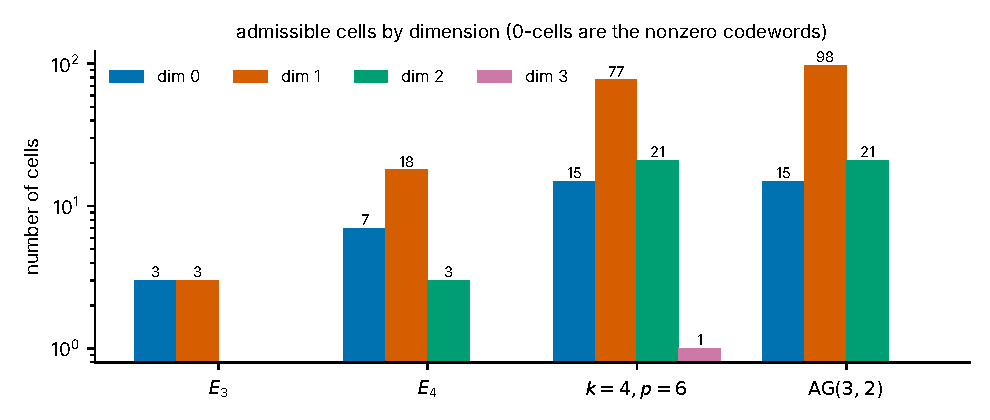
\includegraphics[width=0.95\textwidth]{figures/fig03_admissible_cells.pdf}
\caption{Numbers of cells of each dimension (dimension $0$ counts the nonzero codewords) for $E_3$, $E_4$, a minimal class with $k=4$, $p=6$, and $\AG(3,2)$. A cell is determined by a family $S$ of disjoint circuits and a coset of $\spn S$ (Lemma~\ref{lem:cellpair}). \figdesc{exact combinatorial data computed by \texttt{scripts/figs.py}; no higher-dimensional geometry is implied by the drawing.}}\label{fig:cells}
\end{figure}

\subsection{Collisions and embeddedness}

\begin{definition}[Collision; embedded]\label{def:collision}
Two \emph{distinct} cells $Z\ne Z'$ of positive dimension \emph{collide} if their relative interiors intersect; equivalently (Theorem~\ref{thm:centre}) if $U(S)=U(T)$ and $x=y$ off $U$. A collision is a pair $\{Z,Z'\}$ of colliding cells. The box is \emph{non-embedded} if it has a collision and \emph{embedded} otherwise.
\end{definition}

The word ``embedded'' is justified by the following description in terms of polyhedral complexes.

\begin{proposition}[Embedded $\Leftrightarrow$ face-to-face]\label{prop:facetoface}
The faces of a cell $Z(S,x)$ are the cells $Z(S',x')$ with $S'\subseteq S$ and $x'$ a vertex of $Z$, together with the vertices. The box is embedded if and only if any two cells (of any dimension) intersect in a common face, possibly empty; i.e.\ if and only if the cells form a polyhedral complex.
\end{proposition}

\begin{proof}
The cell is a product of segments, one per block, so its faces are the sub-products: choose a subfamily $S'\subseteq S$ to vary and fix every other block at one of its two endpoints; the result is $Z(S',x')$ with $x'$ a vertex (then $x'\notin\spn S'$, because $x'\oplus s'$ is a vertex of $Z$, hence nonzero, for every $s'\in\spn S'\subseteq\spn S$). If a collision $\{Z,Z'\}$ exists, the common centre lies in $Z\cap Z'$; if $Z\cap Z'$ were a face $G$ of both, then $G\ni\gamma$ with $\gamma\in\relint Z$ forces $G=Z$ (a face containing a point of the relative interior is the whole cell), and likewise $G=Z'$, so $Z=Z'$, a contradiction. Conversely suppose there is no collision, and let $Z,Z'$ be cells with $p\in Z\cap Z'$. The unique face $G$ of $Z$ with $p\in\relint G$ and the unique face $G'$ of $Z'$ with $p\in\relint G'$ are cells or vertices; if $G$ is a vertex then $p\in F$ is a $0/1$ point, and then $G'$ is also a vertex because the relative interior of a positive-dimensional cell contains no $0/1$ points (Lemma~\ref{lem:relint}); in the positive-dimensional case $\relint G\cap\relint G'\ne\emptyset$ and no collision forces $G=G'$. So every point of $Z\cap Z'$ lies in the relative interior of a common face. Taking $p$ to be the average of points chosen in the relative interiors of the common faces of maximal dimension, the minimal face of $Z$ containing $p$ is a common face containing all of them; hence $Z\cap Z'$ is a single common face.
\end{proof}

\subsection{Witnesses and ranks}

\begin{definition}[Witness; witness rank; $\rmin$]\label{def:witness}
Let $\{Z,Z'\}$ be a collision with generator matrices $A\,(r\times n)$ and $B\,(t\times n)$ and base points $x,y$; put $\delta=x-y$. The triple $(A,B,\delta)$ is a \emph{witness}. Its \emph{witness rank} is
\[
d_{\mathrm{span}}=\rk\begin{bmatrix}A\\ B\\ \delta\end{bmatrix}.
\]
The \emph{minimum witness rank} $\rmin(C)$ of a non-embedded box is the minimum of the witness rank over all collisions.
\end{definition}

\begin{lemma}[Witness rank is the dimension of the affine span]\label{lem:rankspan}
For a collision $\{Z,Z'\}$ the vector $\delta$ lies in the row space of $\begin{bmatrix}A\\B\end{bmatrix}$. Consequently the witness rank equals $\rk\begin{bmatrix}A\\B\end{bmatrix}$ and equals the dimension of the affine hull of $Z\cup Z'$. It is at least $\max(r,t)$ and at most $r+t$.
\end{lemma}

\begin{proof}
Let $\gamma$ be the common centre. Then $\gamma=x+\tfrac12\sum g_j=y+\tfrac12\sum h_l$ (rows $g_j$ of $A$, $h_l$ of $B$), so $\delta=x-y=\tfrac12\sum h_l-\tfrac12\sum g_j$. The affine hulls of $Z$ and $Z'$ are $\gamma+\mathrm{row}(A)$ and $\gamma+\mathrm{row}(B)$, so the hull of the union is $\gamma+\mathrm{row}(A)+\mathrm{row}(B)$. The rows of $A$ are independent (disjoint supports), similarly for $B$.
\end{proof}

\begin{remark}[Individual versus minimum]\label{rem:individual}
A collision may have witness rank larger than $3$; the quantity $\rmin$ takes the minimum. For instance the even-weight code $E_6$ (Section~\ref{sec:E4}) has $1710$ collisions: $720$ between cells of dimensions $(2,2)$ and $990$ between cells of dimensions $(3,3)$, with witness ranks $3,4,5,6$ occurring $585,360,585,180$ times (exact enumeration with the engine of Appendix~\ref{app:repro}), while the minimum is still $3$. Only the minimum is bounded.
\end{remark}

\begin{example}[An embedded box, $E_3$]\label{ex:E3}
Let $M=(1\,1\,1)$, $C=E_3=\{000,110,101,011\}$. The circuits are the three weight-two words, pairwise intersecting. A circuit family contains only one circuit, so all cells are $1$-dimensional: the cell of the circuit $c$ and base point $x\in C\setminus\{0,c\}$ joins the two remaining words (for $c=110$, $x=101$, the edge $101$--$011$). The fibre is a triangle with three edges, the cells form a complex, and the box is embedded; Theorem~\ref{thm:E1} below shows this without enumeration, since no set has two partitions.
\end{example}

\begin{figure}[ht]
\centering
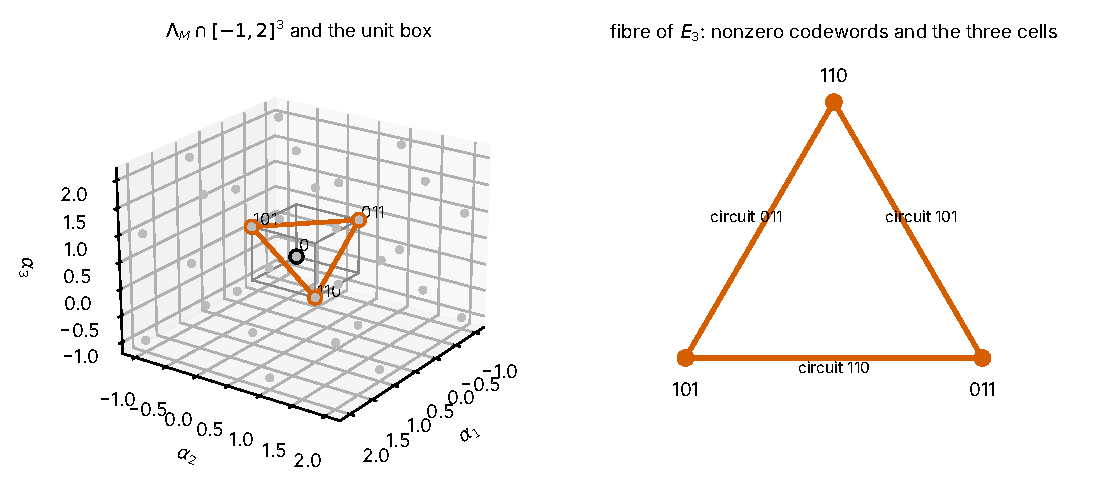
\includegraphics[width=0.92\textwidth]{figures/fig01_lattice_slice.pdf}
\caption{The binary relation lattice and its $0/1$ slice for $n=3$, $M=(1\,1\,1)$. Left: lattice points of $\Lambda_M$ in $\{-1,0,1,2\}^3$ (grey) and the unit box; the three nonzero fibre points $110,101,011$ are the vertices of the triangle (the edges are the three admissible cells). Right: the same data as codewords of $E_3$. \figdesc{exact integer coordinates generated by \texttt{scripts/figs.py}; a rendering of $n=3$ only, not of higher-dimensional geometry.}}\label{fig:lattice}
\end{figure}

\begin{figure}[ht]
\centering
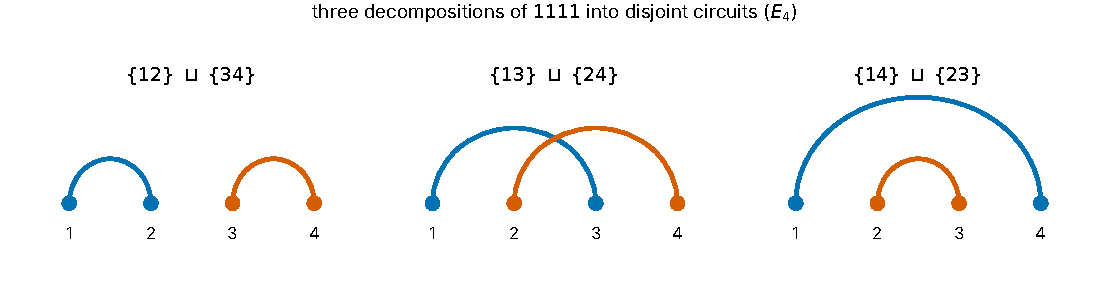
\includegraphics[width=0.92\textwidth]{figures/fig02_circuit_decompositions.pdf}
\caption{Circuits and decompositions in $E_4$. The word $1111$ has three distinct decompositions into pairs of disjoint circuits. \figdesc{generated by \texttt{scripts/figs.py} from the exact circuit list.}}\label{fig:decomp}
\end{figure}

%% ===================================================================
%% PART II
%% ===================================================================
\part{Circuit structure of non-embedded boxes}

%% -------------------------------------------------------------------
\section{The exact circuit-partition criterion}\label{sec:E1}

\begin{lemma}\label{lem:notunion}
A vector space $V$ over $\F_2$ is not the union of two proper subspaces.
\end{lemma}

\begin{proof}
If $\dim V=d$ and $A,B\subsetneq V$ are subspaces, then $|A\cup B|\le|A|+|B|-1\le2\cdot2^{d-1}-1<2^d$ because $0\in A\cap B$.
\end{proof}

(The statement is false for \emph{three} subspaces over $\F_2$, as the three lines of a plane show. This is why the criterion below is formulated with \emph{two} partitions.)

\begin{theorem}[Circuit-partition criterion; \gid{G10-E1}]\label{thm:E1}
For a code $C\le\F_2^n$ the following are equivalent.
\begin{enumerate}[label=(\roman*)]
\item The box $C$ is non-embedded.
\item There is a set $U\subseteq[n]$ with $|\Part_U(C)|\ge2$, i.e.\ $U$ has two distinct partitions into circuits.
\item Some word of $C$ has two distinct decompositions into disjoint circuits.
\end{enumerate}
Moreover, if $S\ne T$ are partitions of $U$ into circuits and $x\in C\setminus(\spn S\cup\spn T)$ (such $x$ exists), then $Z(S,x)$ and $Z(T,x)$ collide.
\end{theorem}

\begin{proof}
(ii)$\Leftrightarrow$(iii) is the identification of a word $\one_U$ with its support.

(ii)$\Rightarrow$(i). Let $S\ne T$ be partitions of $U$. By Lemma~\ref{lem:proper}, $\spn S$ and $\spn T$ are proper subspaces of $C_U\le C$, hence of $C$. By Lemma~\ref{lem:notunion} there is $x\in C\setminus(\spn S\cup\spn T)$. The cells $Z(S,x)$ and $Z(T,x)$ exist, have the same union $U$, agree (trivially) off $U$ because they have the same base point, and are different because $S\ne T$ (Lemma~\ref{lem:cellpair}). By Theorem~\ref{thm:centre} they collide.

(i)$\Rightarrow$(ii). Let $\{Z(S,x),Z(T,y)\}$ be a collision, so $U(S)=U(T)=:U$ and $x=y$ off $U$. If $S\ne T$ these are two distinct partitions of $U$. Suppose $S=T$. By Lemma~\ref{lem:cellpair} the cells are distinct, so $c:=x\oplus y\notin\spn S$; and $c\in C$ with $\supp c\subseteq U$ since $x=y$ off $U$. In particular $c\ne0$. By Lemma~\ref{lem:circuit-basic}(b) write $c=c_1\sqcup\dots\sqcup c_q$ as a disjoint union of circuits (all inside $U$). The word $\one_U\oplus c$ lies in $C$ (because $\one_U=\bigoplus S_j\in C$) and has support $U\setminus\supp c$; if this is nonempty write it as a disjoint union of circuits $d_1\sqcup\dots\sqcup d_s$. Then $S'=\{c_1,\dots,c_q,d_1,\dots,d_s\}$ is a partition of $U$ into circuits. If $S'=S$, every block of $S$ would lie either inside $\supp c$ or inside $U\setminus\supp c$, so $c$ would be a union of blocks of $S$, i.e.\ $c\in\spn S$, which is false. So $S'\ne S$ and $U$ has two distinct partitions.
\end{proof}

\src{\gid{G10-E1}, GEO-I v010, \texttt{MATHEMATICS.md} \S1.1 (\PROVED). The proof above uses only Lemmas~\ref{lem:proper} and~\ref{lem:notunion} and Theorem~\ref{thm:centre}. It was re-derived independently of the release text, and the equivalence (i)$\Leftrightarrow$(ii) was cross-checked by exhaustive computation on $4213$ small codes against a direct enumeration of cells and relative-interior intersections (Appendix~\ref{app:repro}); no discrepancy.}

\begin{remark}[Geometric content]\label{rem:E1geo}
Theorem~\ref{thm:E1} turns a metric--geometric property (overlap of relative interiors of parallelepipeds in $\R^n$) into a purely \emph{linear-algebraic} one (non-uniqueness of a decomposition into minimal supports). Two features are worth recording. First, the collision produced in (ii)$\Rightarrow$(i) uses a \emph{common} base point $x$ for both cells; collisions of this kind are the ones to which the rank-three construction of Section~\ref{sec:L5} applies. Second, in (i)$\Rightarrow$(ii) a collision with $S=T$ and distinct cosets forces a \emph{third} partition: this is the only place where one needs that every nonzero word is a union of circuits.
\end{remark}

\begin{proposition}[Cells through a centre]\label{prop:centre-count}
Let $U\subseteq[n]$ with $\one_U\in C$, let $C_U=\{w\in C:\supp w\subseteq U\}$ and let $z\in\F_2^{[n]\setminus U}$ be such that $X_z=\{x\in C: x|_{[n]\setminus U}=z\}$ is nonempty. The number of cells of positive dimension whose union is $U$ and whose base point agrees with $z$ off $U$ (that is, the cells whose relative interior contains the centre $\gamma(U,z)$) is
\[
N(U,z)=\sum_{S\in\Part_U(C)}\Bigl(\frac{|C_U|}{2^{|S|}}-[z=0]\Bigr).
\]
In particular, if $\one\in C$, then the number of cells whose centre is $(\tfrac12,\dots,\tfrac12)$ is $N=\sum_{P\in\Part}(2^{k-m_P}-1)$, with $m_P=|P|$ and $k=\dim C$, and the number of collisions with this centre is $\binom N2$.
\end{proposition}

\begin{proof}
$X_z$ is a coset of $C_U$ (the difference of two elements has support in $U$), so $|X_z|=|C_U|$. By Lemma~\ref{lem:cellpair} the cells over $(S,z)$ correspond to cosets of $\spn S\le C_U$ in $X_z$, excluding the coset $\spn S$ itself, which occurs inside $X_z$ exactly when $z=0$. The coset count is $|C_U|/2^{|S|}$ (Lemma~\ref{lem:span}). For $U=[n]$ the set $X_z$ is $C$ itself.
\end{proof}

\begin{corollary}[Collisions of a minimal box]\label{cor:collcount}
In a minimal non-embedded box every cell with $U=[n]$ has centre $\tfrac12\one$, every collision has this centre (Theorem~\ref{thm:F1}), and any two distinct cells with union $[n]$ collide. Hence the number of collisions is exactly $\binom N2$ with $N=\sum_{P\in\Part}(2^{k-m_P}-1)$.
\end{corollary}

\begin{proof}
A collision has a common union $U$ with two partitions, so $U=[n]$ by Theorem~\ref{thm:F1}; for $U=[n]$ the condition ``equal off $U$'' is empty, so any two distinct cells with union $[n]$ collide (Theorem~\ref{thm:centre}).
\end{proof}

\src{New here: this closed formula was not found in the release files read. It was verified by direct enumeration of cells for the $k=3,4,5$ classes (Appendix~\ref{app:repro}); e.g.\ $E_4$ has $N=3$ ($3$ collisions), the $k=4$, $p=6$ box has $N=13$ ($78$ collisions) and the $k=5$, $p=8$ box has $N=57$ ($1596$ collisions), in agreement with the direct enumeration of all collisions (Section~\ref{sec:E4}).}

%% -------------------------------------------------------------------
\section{Minimal non-embedded boxes and shortening}\label{sec:minimal}

\subsection{Shortening}

\begin{definition}[Shortening]\label{def:shortening}
For $i\in[n]$ the \emph{shortening} of $C$ at $i$ is the code $C_{(i)}=\{w|_{[n]\setminus\{i\}}:\ w\in C,\ w_i=0\}\le\F_2^{n-1}$. It is the kernel of the parity matrix with the $i$th column deleted. For $I\subseteq[n]$ write $C_{(I)}$ for the iterated shortening. The box $C_{(i)}$ is called a \emph{sub-box} of $C$.
\end{definition}

Deleting a column of $M$ corresponds geometrically to fixing the coordinate $i$ of every lattice vector at $0$: the lattice $\Lambda_{M'}$ of the deleted matrix is the intersection of $\Lambda_M$ with $\{\alpha_i=0\}$, and the box $[0,1]^{n-1}$ is the corresponding face of $[0,1]^n$.

\begin{lemma}[Circuits and cells of a shortening]\label{lem:shortcirc}
(a)~The circuits of $C_{(i)}$ are exactly the circuits of $C$ not containing $i$.
(b)~A circuit family of $C_{(i)}$ is a circuit family of $C$ avoiding $i$; the cells of $C_{(i)}$ are the cells $Z(S,x)$ of $C$ with $i\notin U(S)$ and $x_i=0$ (with coordinate $i$ deleted).
(c)~Two cells of $C_{(i)}$ collide if and only if the corresponding cells of $C$ collide, and the generator matrices of the pair differ only by an added zero column; so the witness ranks agree.
\end{lemma}

\begin{proof}
(a)~A word of $C_{(i)}$ is a word of $C$ vanishing at $i$. If $c$ is a circuit of $C$ with $i\notin c$ then every word of $C$ with support inside $c$ vanishes at $i$, so minimality in $C$ gives minimality in $C_{(i)}$. Conversely a circuit of $C_{(i)}$ is the support of a word of $C$ vanishing at $i$, and every word of $C$ with smaller support also vanishes at $i$, so it is a circuit of $C$ avoiding $i$. (b)~follows from (a) and the definition of cells, since $x\in C_{(i)}$ means $x\in C$, $x_i=0$. (c)~The condition ``same union and equal off the union'' reads the same in $\F_2^{n-1}$ and in $\F_2^n$ when $x_i=y_i=0$ and $i$ lies outside the common union.
\end{proof}

\begin{definition}[Minimal box]\label{def:minimal}
A box $C$ is \emph{minimal} (more fully: \emph{coordinatewise-minimal non-embedded}) if $C$ is non-embedded and $C_{(i)}$ is embedded for every $i\in[n]$.
\end{definition}

\begin{proposition}[Descent to a minimal sub-box]\label{prop:descent}
Every non-embedded box $C$ has a minimal sub-box $C_{(I)}$, $I\subseteq[n]$, and $\rmin(C)\le\rmin(C_{(I)})$.
\end{proposition}

\begin{proof}
If $C$ is non-embedded and not minimal, some $C_{(i)}$ is non-embedded and has length $n-1$. Repeat; the process stops because the length decreases at every step. By Lemma~\ref{lem:shortcirc}(c) every collision of $C_{(I)}$ lifts to a collision of $C$ with the same witness rank, so $\rmin(C)\le\rmin(C_{(I)})$.
\end{proof}

\src{\gid{G9-T5} (reduction to minimal boxes), GEO-I v009 \texttt{MATHEMATICS.md} \S2.4 (\PROVED+\CHECKED); the argument above is the general reduction without reference to nullity.}

\begin{corollary}[Nullity at least three]\label{cor:nullity}
If $C$ is non-embedded then $k=\dim C\ge3$.
\end{corollary}

\begin{proof}
By Theorem~\ref{thm:E1} there are partitions $S\ne T$ of some $U$. By Lemma~\ref{lem:proper}, $2\le|S|=\dim\spn S<\dim C_U\le k$, so $k\ge3$.
\end{proof}

\src{\gid{B-NULL$'$}, GEO-I v008 \texttt{MINIMAL\_RANK.md} (\PROVED): any collision forces nullity $\ge3$.}

\begin{figure}[ht]
\centering
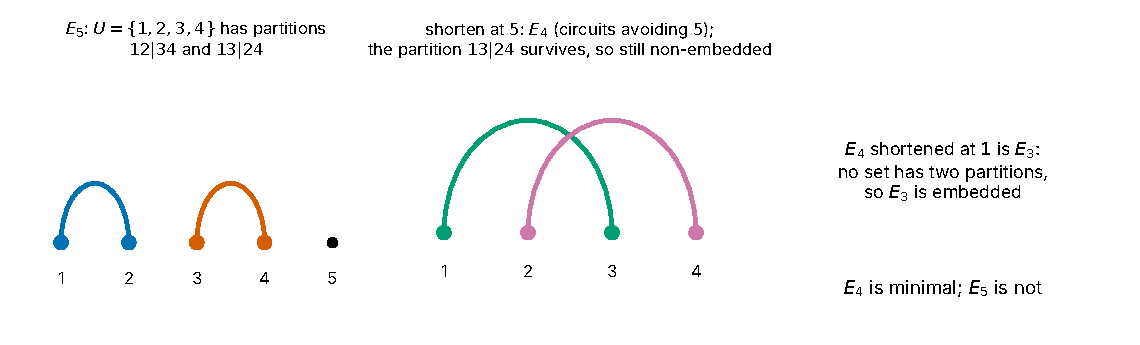
\includegraphics[width=0.95\textwidth]{figures/fig06_shortening.pdf}
\caption{Shortening a coordinate: deleting a parity column keeps exactly the circuits avoiding that coordinate. \figdesc{exact combinatorial data computed by \texttt{scripts/figs.py}; no higher-dimensional geometry is implied by the drawing.}}\label{fig:shortening}
\end{figure}

\subsection{Series classes and reduced boxes}\label{sec:series}

\begin{definition}[Series classes]\label{def:series}
Coordinates $i,j$ are \emph{series-equivalent} if $w_i=w_j$ for all $w\in C$. A coordinate is \emph{dead} if $w_i=0$ for all $w\in C$. The \emph{reduced length} $p(C)$ is the number of series classes of non-dead coordinates; the \emph{multiplicity} of a class is its size. The \emph{reduced code} $\bar C\le\F_2^{p}$ is obtained by keeping one coordinate from every class of non-dead coordinates (and deleting dead ones); $C$ is a \emph{blow-up} of $\bar C$ (plus dead coordinates).
\end{definition}

(In the generator-matrix picture of Section~\ref{sec:affine}, series-equivalent coordinates are the equal columns, and dead coordinates are the zero columns of a generator matrix; ``series'' and ``parallel'' are matroid names for the same relation, depending on whether one reads the code or its dual \cite{Oxley2011}. We use ``series''.)

\begin{proposition}[Blow-up invariance; \gid{B-SERIES}]\label{prop:series}
Let $C$ have no dead coordinates. The words of $C$ are constant on series classes, and replacing every class by a single coordinate gives an isomorphism $C\cong\bar C$ of codes. Under this isomorphism:
\begin{enumerate}[label=(\alph*)]
\item the circuits of $C$ are the preimages of the circuits of $\bar C$ (so every circuit is a union of classes);
\item cells correspond to cells, collisions to collisions; the generator matrices differ by duplicating columns, so witness ranks coincide and $\rmin(C)=\rmin(\bar C)$;
\item $C$ is non-embedded iff $\bar C$ is; and $C$ is minimal iff $\bar C$ is minimal.
\end{enumerate}
If $C$ has dead coordinates, the dead coordinates are in no circuit and in no cell; $C$ is non-embedded iff the code without the dead coordinates is, and then $C$ is not minimal.
\end{proposition}

\begin{proof}
Constancy on classes holds by definition and gives the isomorphism. Supports correspond to unions of classes and inclusion is preserved, so (a) follows; (b)~follows because union, equality off the union, and the cell data $(S,x)$ all transfer, and duplicating columns of a matrix does not change its row rank. For (c): non-embeddedness transfers by~(b). For minimality note that the circuits of $C_{(i)}$ are the circuits of $C$ avoiding $i$ (Lemma~\ref{lem:shortcirc}); these are the preimages of the circuits of $\bar C$ avoiding the class of $i$, i.e.\ the circuits of $\bar C_{(\bar\imath)}$; by Theorem~\ref{thm:E1} embeddedness of a shortening depends only on its circuits and the sets they form, so $C_{(i)}$ is embedded iff $\bar C_{(\bar\imath)}$ is. The statement on dead coordinates holds since a dead coordinate lies in no support, and $C_{(i)}$ for a dead $i$ is the code with $i$ deleted.
\end{proof}

\src{\gid{B-SERIES}, GEO-I v008 \texttt{MINIMAL\_RANK.md} (\PROVED+\CHECKED). Reproved above via Theorem~\ref{thm:E1}.}

\begin{remark}
A blow-up of a minimal box is minimal, although shortening a coordinate of a class of size $\ge2$ turns the other coordinates of the class into dead ones (zero columns of the generator matrix). This is consistent with Proposition~\ref{prop:series} because dead coordinates are irrelevant for embeddedness. Hence the classification of minimal boxes reduces to the classification of reduced minimal boxes plus multiplicities, and all rank statements for reduced boxes carry over to all lengths $n$ (Section~\ref{sec:classify}).
\end{remark}

%% -------------------------------------------------------------------
\section{The full-support theorem and zero-column exclusion}\label{sec:fullsupport}

\begin{theorem}[Full support; \gid{G10-F1}]\label{thm:F1}
Let $C$ be a minimal non-embedded box. If $U\subseteq[n]$ has two distinct partitions into circuits then $U=[n]$. Consequently $\one\in C$, the set $[n]$ has at least two partitions into circuits, and every coordinate lies in a circuit.
\end{theorem}

\begin{proof}
Let $S\ne T$ be partitions of $U$ and suppose $i\notin U$. All circuits of $S$ and $T$ avoid $i$, so by Lemma~\ref{lem:shortcirc}(a) they are circuits of $C_{(i)}$ and $S\ne T$ are two partitions of $U$ in $C_{(i)}$. By Theorem~\ref{thm:E1}, $C_{(i)}$ is non-embedded, contradicting minimality. By Theorem~\ref{thm:E1} some $U$ has two partitions; hence $U=[n]$ is the only such set. The word $\one=\one_{[n]}$ is then a sum of circuits, hence lies in $C$.
\end{proof}

\src{\gid{G10-F1}, GEO-I v010 \texttt{MATHEMATICS.md} \S1.2 (\PROVED); closes the earlier conjecture \gid{G8-C3} (status \textsc{corrected}: formerly open, now proved). This is an immediate consequence of the shortening lemma and Theorem~\ref{thm:E1}.}

\begin{proposition}[No singleton circuits; \gid{G9-Z}, \gid{G11-L5c}]\label{prop:nosingleton}
If $e_i\in C$ for some $i$ (that is, $\{i\}$ is a circuit; equivalently the $i$th parity column vanishes) and $C$ is non-embedded, then $C_{(i)}$ is non-embedded. Consequently a minimal non-embedded box has no circuit of size~$1$: every circuit has at least two coordinates, and there is no zero parity column.
\end{proposition}

\begin{proof}
Let $S\ne T$ be partitions of a set $U$ (Theorem~\ref{thm:E1}). If $i\notin U$ both are partitions in $C_{(i)}$ and we are done by Lemma~\ref{lem:shortcirc}. If $i\in U$, let $S_j\ni i$ be the block of $S$ containing $i$. Since $\{i\}$ is a circuit and circuits are not nested (Lemma~\ref{lem:circuit-basic}(c)), $S_j=\{i\}$; likewise $\{i\}\in T$. Then $S\setminus\{\{i\}\}$ and $T\setminus\{\{i\}\}$ are two different partitions of $U\setminus\{i\}$ (different because $S\ne T$; if one of them is empty then $S=\{\{i\}\}$, and $T$, being a partition of the same set containing $\{i\}$, would equal it). Both avoid $i$, so $C_{(i)}$ is non-embedded.
\end{proof}

\src{\gid{G9-Z}, GEO-I v009 \texttt{MATHEMATICS.md} \S1 (\PROVED+\CHECKED); \gid{G11-L5c}, GEO-I v011 \texttt{MATHEMATICS.md} \S1.1 (\PROVED). The two statements in the release files are proved by separate arguments; the single argument above gives both.}

\begin{corollary}[Properties of a minimal box]\label{cor:minprops}
A minimal non-embedded box $C$ of nullity $k$ satisfies: (P1)~$\one\in C$ and $|\Part|\ge2$; (P2)~no coordinate is dead; every circuit has at least two coordinates; (P3)~$k\ge3$ and $\one$ is not a circuit; (P4)~every partition of $\one$ has $m_P\ge2$ blocks of size $\ge2$ each.
\end{corollary}

\begin{proof}
(P1)~Theorem~\ref{thm:F1}. (P2)~$\one\in C$ has full support, and Proposition~\ref{prop:nosingleton}. (P3)~Corollary~\ref{cor:nullity}; if $\one$ were a circuit then every circuit equals $\one$ and $\Part$ has a single element. (P4)~is (P2) together with (P3).
\end{proof}

%% -------------------------------------------------------------------
\section{Affine-geometric reduction}\label{sec:affine}

\subsection{Generator matrices and point sets}

Let $C\le\F_2^n$ be a code of dimension $k$ without dead coordinates. Choose a basis $b_1,\dots,b_k$ of $C$ and let $G$ be the $k\times n$ matrix with rows $b_s$. Its columns $g_1,\dots,g_n\in\F_2^k\setminus\{0\}$ satisfy
\[
w_f:=\bigl(f\cdot g_i\bigr)_{i\in[n]}\in C,\qquad C=\{w_f:\ f\in\F_2^k\},\qquad f\mapsto w_f\ \text{bijective}.
\]
Thus a code of dimension $k$ without dead coordinates is a \emph{multiset} of nonzero points of $F_2^k$ spanning $\F_2^k$ (the column multiset), up to the action of $\GL(k,2)$ (change of basis of $C$) and permutation of coordinates. Series classes are the sets of coordinates with equal columns; the reduced code corresponds to the set $X=\{g_i\}$ of \emph{distinct} columns, $|X|=p$, spanning $\F_2^k$.

\begin{lemma}\label{lem:equivalence}
Two reduced codes $\bar C,\bar C'$ with point sets $X,X'\subseteq\F_2^k\setminus\{0\}$ (spanning) are equal up to a permutation of coordinates if and only if $X'=\sigma X$ for some $\sigma\in\GL(k,2)$.
\end{lemma}

\begin{proof}
If $\pi\bar C=\bar C'$ for a coordinate permutation $\pi$, then $G'\Pi=AG$ for an invertible $A$ (two generator matrices of the same code differ by a change of basis), so the column of $G'$ at position $\pi(i)$ is $Ag_i$: $X'=AX$. Conversely if $X'=\sigma X$ then $G'$, whose columns are $\sigma g_i$ in some order, generates $\{f\cdot\sigma g_i\}=\{(\sigma^{\top}f)\cdot g_i\}$, the same code up to the coordinate order.
\end{proof}

\begin{figure}[ht]
\centering
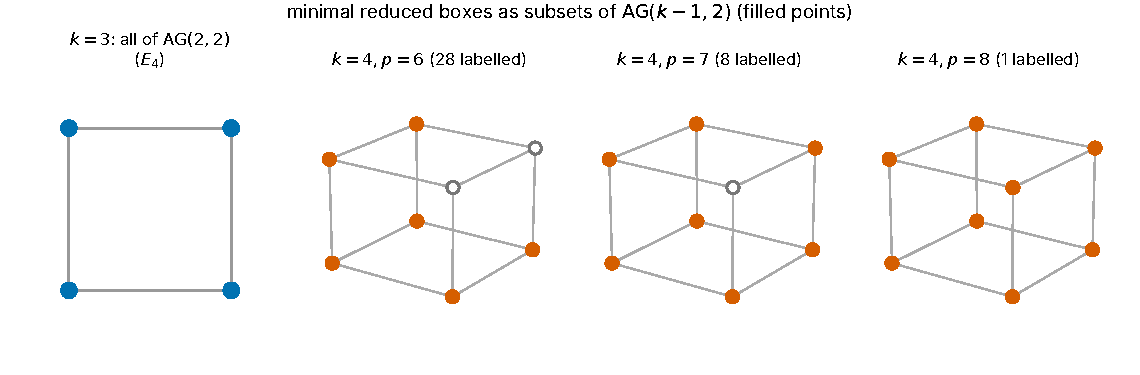
\includegraphics[width=0.95\textwidth]{figures/fig07_affine_reduction.pdf}
\caption{Affine reduction: the reduced coordinate set as a point set in an affine space. \figdesc{exact combinatorial data computed by \texttt{scripts/figs.py}; no higher-dimensional geometry is implied by the drawing.}}\label{fig:affred}
\end{figure}

\subsection{The affine hyperplane}

Since $\one\in C$ for minimal boxes (Theorem~\ref{thm:F1}) there is a unique $f_0\in\F_2^k$ with $w_{f_0}=\one$, i.e.\ $f_0\cdot g_i=1$ for all $i$. The set $H=\{x\in\F_2^k: f_0\cdot x=1\}$ is an affine hyperplane, in bijection with $\F_2^{k-1}$ after choosing coordinates in which $f_0=e_k^*$, and its affine structure is that of the affine space $\AG(k-1,2)$ (the points of $H$ are the vectors with last coordinate $1$). The subgroup of $\GL(k,2)$ preserving $H$ (equivalently fixing $f_0$) acts on $H$ as the full affine group $\AGL(k-1,2)$.

\begin{theorem}[Affine reduction; \gid{G10-A1}]\label{thm:affine}
Let $C$ be a minimal non-embedded box of nullity $k$ and $X\subseteq\F_2^k$ its reduced point set, $p=|X|$. Then:
\begin{enumerate}[label=(\alph*)]
\item $X\subseteq H\cong\AG(k-1,2)$ and $X$ spans $\F_2^k$ (equivalently, $X$ is not contained in any proper affine subspace of $H$);
\item $p\ge k+1$; and $p=k+1$ holds if and only if $C=E_p$ (and then $p=4$, $k=3$);
\item two minimal boxes have isomorphic reduced codes iff their reduced point sets lie in the same $\AGL(k-1,2)$-orbit of subsets of $H$.
\end{enumerate}
Conversely, for every spanning subset $X\subseteq H$ the code $C(X)=\{(f\cdot x)_{x\in X}\}$ has dimension $k$ and contains $\one$; whether it is non-embedded, and whether it is minimal, depends on $X$ only through its $\AGL(k-1,2)$-orbit.
\end{theorem}

\begin{proof}
(a)~$\one\in C$ gives $X\subseteq H$; $X$ spans because the generator matrix has rank $k$; and ``spans $\F_2^k$'' means that $X$ is not contained in a proper linear subspace; since $X\subset H$ and $0\notin H$, this means $X$ is not contained in a proper affine subspace of $H$.

(b)~$p=k$ would make $X$ a basis, so $C=\F_2^p$ with all singletons as circuits, contradicting Proposition~\ref{prop:nosingleton}. For $p=k+1$ the relations among the columns form a $1$-dimensional space $\langle a\rangle=C^\perp$, hence $C=a^\perp$. If $a_i=0$ then $e_i\in C$, a singleton circuit; so $a=\one$, $C=\one^\perp=E_p$. (The circuits of $E_p$ are the weight-two words, and $E_p$ is minimal only for $p=4$, Proposition~\ref{prop:Emin}.)

(c)~Lemma~\ref{lem:equivalence} gives equivalence under $\GL(k,2)$. If $\sigma X=X'$ and both sets lie in $H$, then $\sigma$ maps $X$ into $H$; because $X$ spans, $f_0\circ\sigma^{-1}$ takes the value $1$ on $X'$, which spans, and is a functional equal to $1$ on a spanning subset of $H$, so $f_0\circ\sigma^{-1}=f_0$ (a functional is determined by its values on a spanning set). So $\sigma$ lies in the stabiliser of $f_0$, which acts on $H$ as $\AGL(k-1,2)$.

The final statement is Lemma~\ref{lem:equivalence} together with the fact that isomorphic codes have the same circuits and hence the same embeddedness and minimality (Theorem~\ref{thm:E1}).
\end{proof}

\src{\gid{G10-A1}, GEO-I v010 \texttt{MATHEMATICS.md} \S1.3 (\PROVED). The statements on $p\ge k+1$ and on $E_p$ are made explicit here.}

\begin{proposition}[The even-weight codes]\label{prop:Emin}
For $p\ge3$ let $E_p=\{w\in\F_2^p:\wt(w)\text{ even}\}$. Its circuits are the $\binom p2$ words of weight two. $E_3$ is embedded, $E_p$ is non-embedded for $p\ge4$, $E_4$ is minimal, and $E_p$ is not minimal for $p\ge5$.
\end{proposition}

\begin{proof}
Every even word of weight $\ge4$ contains a weight-two word, so the circuits are the pairs. A family of disjoint pairs is a partial matching; $E_3$ has no two disjoint pairs, so the families are single pairs and every set has at most one partition: embedded. For $p\ge4$ the set $\{1,2,3,4\}$ has the partitions $\{12,34\}$ and $\{13,24\}$: non-embedded. Shortening $E_p$ at a coordinate gives $E_{p-1}$ (the words vanishing at $i$ are the even words on the other coordinates), so $E_4$ has the embedded shortening $E_3$, while for $p\ge5$ the shortening $E_{p-1}$ with $p-1\ge4$ is non-embedded.
\end{proof}

\subsection{Consequences}

Theorem~\ref{thm:affine} reduces the study of minimal boxes to the study of subsets of the finite affine spaces $\AG(k-1,2)$ up to affine equivalence. It also fixes the extreme case: the full affine space $X=\AG(k-1,2)$, which gives the first-order Reed--Muller code $\mathrm{RM}(1,k-1)$ of length $2^{k-1}$ (Proposition~\ref{prop:RM}). All the arithmetic below is done with $k$ (the dimension of the ambient space $\F_2^k$), $p$ (the number of points) and the partition data of $X$.

%% -------------------------------------------------------------------
\section{Collision rank and local rank-three extraction}\label{sec:L5}

\begin{lemma}[Lower bound; \gid{B-LOW}]\label{lem:LOW}
Every collision has witness rank at least $3$. Consequently $\rmin(C)\ge3$ for every non-embedded box.
\end{lemma}

\begin{proof}
Let $\{Z(S,x),Z(T,y)\}$ be a collision, $r=|S|,t=|T|$, with generators $g_j$ and $h_l$. By Lemma~\ref{lem:rankspan} the witness rank is at least $\max(r,t)$, so we may assume $r,t\le2$.

\emph{Case $r=1$.} Then $U=S_1$ is a circuit, so every circuit inside $U$ equals $U$ and $T=\{U\}=S$. As $x=y$ off $U$, the word $c=x\oplus y$ has support in $U$, so $c\in\{0,U\}=\spn S$ (Lemma~\ref{lem:circuit-basic}(c)), and $Z(S,x)=Z(S,y)$ by Lemma~\ref{lem:cellpair}, a contradiction. The case $t=1$ is symmetric. So $r=t=2$.

\emph{Case $r=t=2$.} Suppose the witness rank equals $2$. Then the rows of $B$ lie in the row space of $A$: $h_l=\lambda_{l1}g_1+\lambda_{l2}g_2$ with real $\lambda$. Since $g_j$ has entries $\pm1$ exactly on $S_j$ and $h_l$ has entries in $\{0,\pm1\}$, $|\lambda_{lj}|\in\{0,1\}$. If both were nonzero then $T_l=S_1\cup S_2=U$ and the other member of $T$ could not be disjoint from it; so each $T_l$ equals $S_1$ or $S_2$, and $T=S$. Then $h_l=\pm g_l$ means $1-2y_i=\varepsilon_l(1-2x_i)$ on $S_l$, i.e.\ $y|_{S_l}=x|_{S_l}$ or $y|_{S_l}=\bar x|_{S_l}$ for each $l$; hence $c=x\oplus y$ is constant on every block, so $c\in\spn S$ (it vanishes off $U$ because $x=y$ there), and the cells coincide: a contradiction. So the rank is at least $3$.
\end{proof}

\src{\gid{B-LOW} (also \gid{G8-T3a}), GEO-I v008 \texttt{MINIMAL\_RANK.md} (\PROVED).}

\begin{theorem}[Local rank-three extraction; \gid{G10-L5}, \gid{B-COMMON}]\label{thm:L5}
Let $a\in C$ be a word with two distinct decompositions into two disjoint circuits, $a=b_1\sqcup b_2=c_1\sqcup c_2$ with $\{b_1,b_2\}\ne\{c_1,c_2\}$. Put $S=\{b_1,b_2\}$, $T=\{c_1,c_2\}$ and choose any $x\in C\setminus(\spn S\cup\spn T)$. Then $Z(S,x)$ and $Z(T,x)$ collide, and their four generators satisfy
\[
g_1+g_2=h_1+h_2=\bigl((1-2x_i)\one_{i\in\supp a}\bigr)_{i\in[n]},
\]
so the witness rank is exactly $3$. In particular $\rmin(C)=3$ for any code that contains such a word.
\end{theorem}

\begin{proof}
Theorem~\ref{thm:E1} gives the collision. On $U=\supp a$ the generators of the two cells are the restrictions of the same vector $s=(1-2x_i)_i$ to the blocks: $g_j=s|_{b_j}$, $h_l=s|_{c_l}$. Hence $g_1+g_2=s|_U=h_1+h_2$, a nontrivial linear relation among four vectors; their span has dimension at most $3$. Lemma~\ref{lem:LOW} gives at least $3$.
\end{proof}

\src{\gid{G10-L5} (= \gid{G10-T5}) and \gid{B-COMMON}, GEO-I v010 \texttt{MATHEMATICS.md} \S1.5 and v008 \texttt{MINIMAL\_RANK.md} (\PROVED).}

\begin{definition}[Condition W2]\label{def:W2}
A box satisfies \emph{W2} if $\one\in C$ and the set $\Part^{(2)}$ of partitions of $\one$ into exactly two circuits has at least two elements; $n_2=|\Part^{(2)}|$.
\end{definition}

\begin{theorem}[Conditional universality; \gid{G10-C1$'$}]\label{thm:C1p}
If every minimal non-embedded box satisfies W2, then $\rmin(C)=3$ for \emph{every} non-embedded box $C$.
\end{theorem}

\begin{proof}
By Proposition~\ref{prop:descent} there is a minimal sub-box $C_{(I)}$ with $\rmin(C)\le\rmin(C_{(I)})$. By W2 the word $\one\in C_{(I)}$ has two distinct two-circuit decompositions, so Theorem~\ref{thm:L5} gives $\rmin(C_{(I)})=3$. Hence $\rmin(C)\le3$, and Lemma~\ref{lem:LOW} gives $\rmin(C)\ge3$.
\end{proof}

\src{\gid{G10-C1$'$}, GEO-I v010 \texttt{MATHEMATICS.md} \S1.5 (\PROVED). The hypothesis W2 for \emph{all} minimal boxes is the content of Theorem~\ref{thm:W2} (Part~III), proved unconditionally in this paper.}

Theorem~\ref{thm:C1p} thus reduces the universal rank statement to a purely combinatorial one: \emph{every minimal non-embedded box has two distinct partitions of the all-ones word into two circuits}. Part~III proves this.

\begin{figure}[ht]
\centering
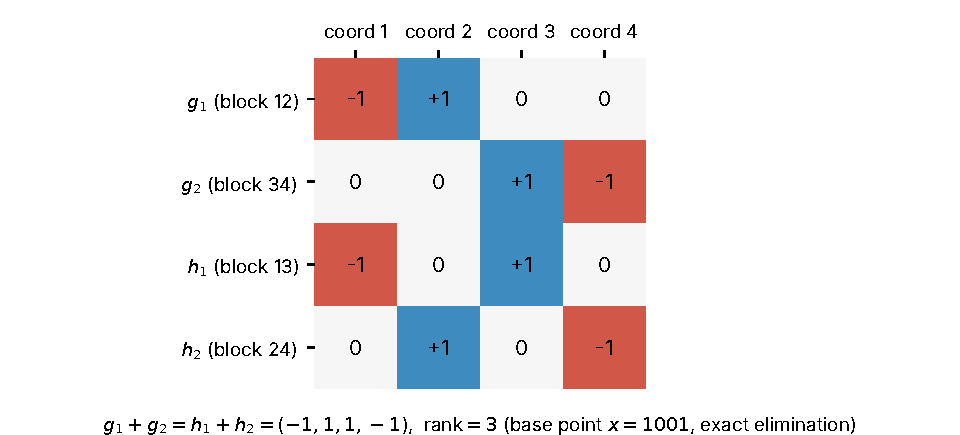
\includegraphics[width=0.95\textwidth]{figures/fig05_rank3_collision.pdf}
\caption{A rank-three collision in $E_4$ with common base point $x=1001$. The four generators of the cells $Z(\{12,34\},x)$ and $Z(\{13,24\},x)$ as a $4\times4$ matrix, and the relation $g_1+g_2=h_1+h_2=(-1,1,1,-1)$. \figdesc{exact integer data; rank computed by exact elimination, \texttt{scripts/figs.py}.}}\label{fig:rank3}
\end{figure}

\begin{figure}[ht]
\centering
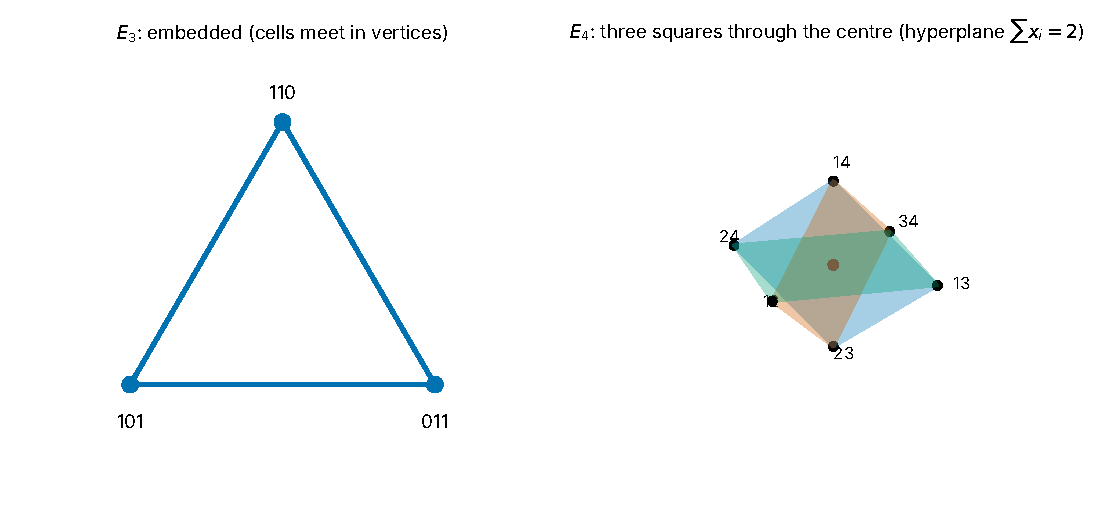
\includegraphics[width=0.95\textwidth]{figures/fig04_embedded_vs_nonembedded.pdf}
\caption{Embedded versus non-embedded. Left: $E_3$ (a triangle; cells meet in vertices). Right: the octahedron of the six weight-two words of $E_4$ in the hyperplane $\sum x_i=2$ with the three equatorial squares, which share diagonals and all contain the centre. \figdesc{an exact subcomplex of the $4$-dimensional cell structure; the vertex $1111$ and the cells through it are omitted. Not a picture of the full cell complex.}}\label{fig:octa}
\end{figure}

%% ===================================================================
%% PART III
%% ===================================================================
\part{Rigidity, vector-space partitions and universality}

Throughout Part~III, $C$ is a \emph{minimal non-embedded box} of nullity $k$. We use the reduced code (Proposition~\ref{prop:series}): $p$ denotes the number of coordinates of the reduced code, which we identify with $C$, so blocks of partitions of $\one$ have sizes measured in the reduced code and $\sum_{B\in P}|B|=p$. All statements in this part are statements about the reduced code; by Proposition~\ref{prop:series} they transfer to blow-ups.

%% -------------------------------------------------------------------
\section{Circuit rigidity}\label{sec:rigidity}

\begin{theorem}[Rigidity; \gid{G10-R}]\label{thm:rigid}
Let $C$ be a minimal non-embedded box. Then:
\begin{enumerate}[label=(\alph*)]
\item every word $w\in C\setminus\{0,\one\}$ has a \emph{unique} decomposition into pairwise disjoint circuits;
\item the word $\one$ has $\beta=|\Part|\ge2$ decompositions;
\item the number of circuit families (nonempty sets of pairwise disjoint circuits) of $C$ is $2^k-2+\beta$, and a family whose union is not $[n]$ is determined by its union.
\end{enumerate}
\end{theorem}

\begin{proof}
(a)~If $w\ne0,\one$ had two decompositions $S\ne T$, the set $U=\supp w\ne[n]$ would have two partitions, contradicting Theorem~\ref{thm:F1}. (b)~is Theorem~\ref{thm:F1}. (c)~Families with union $\ne[n]$ correspond bijectively to words $w\in C\setminus\{0,\one\}$ (each such word has exactly one decomposition, by~(a), and each family determines its union word); there are $2^k-2$ such words. The families with union $[n]$ are the $\beta$ elements of $\Part$.
\end{proof}

\src{\gid{G10-R}, GEO-I v010 \texttt{MATHEMATICS.md} \S1.4 (\PROVED): rigidity and the count of families. The proof above is a direct consequence of Theorem~\ref{thm:F1}.}

The converse also holds and shows that rigidity is not just a consequence but a characterisation.

\begin{proposition}[Rigidity characterises minimality]\label{prop:rigid-char}
A code $C$ with $\one\in C$ is minimal non-embedded if and only if $\one$ has at least two decompositions into disjoint circuits and every $w\in C\setminus\{0,\one\}$ has exactly one.
\end{proposition}

\begin{proof}
($\Rightarrow$)~Theorem~\ref{thm:rigid}. ($\Leftarrow$)~$C$ is non-embedded by Theorem~\ref{thm:E1}. Let $i\in[n]$. A nonzero word of $C_{(i)}$ is a word $w\in C$ with $w_i=0$, so $w\ne\one$ and $w$ has a unique decomposition into circuits of $C$; these circuits lie in $\supp w$, so they avoid $i$ and are circuits of $C_{(i)}$ (Lemma~\ref{lem:shortcirc}). Hence no word of $C_{(i)}$ has two decompositions in $C_{(i)}$, and $C_{(i)}$ is embedded by Theorem~\ref{thm:E1}.
\end{proof}

\src{The converse is noted here; it was not found stated in the release files read.}

The bijection of words and circuit families in Theorem~\ref{thm:rigid} makes the combinatorics of a minimal box unusually rigid: the family structure is that of a \emph{linear space with exactly one failure of unique factorisation}, and the next section shows that this single failure is organised by a vector-space partition.

%% -------------------------------------------------------------------
\section{Vector-space partitions from partitions of the all-ones word}\label{sec:vsp}

Recall that $\Part$ is the set of partitions $P$ of $[n]$ (in the reduced code, of the $p$ coordinates) into circuits; $m_P=|P|\ge2$ is the number of blocks (Corollary~\ref{cor:minprops}), and each block has size $\ge2$. Put
\[
V_P=\spn P=\Bigl\{\bigoplus_{B\in J}B:\ J\subseteq P\Bigr\}\le C,\qquad\dim V_P=m_P,\qquad\{0,\one\}\subseteq V_P.
\]
(Lemma~\ref{lem:span}.)

\begin{lemma}[Existence]\label{lem:vsp-exist}
Every $w\in C\setminus\{0,\one\}$ lies in $V_P$ for at least one $P\in\Part$.
\end{lemma}

\begin{proof}
Both $w$ and $\one\oplus w$ are nonzero words of $C$ (neither equals $\one$ or $0$ because $w\ne0,\one$). Decompose each into disjoint circuits (Lemma~\ref{lem:circuit-basic}(b)); their supports are complementary, so the union of the two decompositions is a partition $P$ of $[n]$ into circuits, and $w$ is the sum of the blocks coming from the decomposition of $w$: $w\in V_P$.
\end{proof}

\begin{lemma}[Uniqueness]\label{lem:vsp-uniq}
If $w\in V_P\cap V_Q$ with $w\ne0,\one$ then $P=Q$.
\end{lemma}

\begin{proof}
Write $w=\bigsqcup_{B\in J}B$ with $J\subseteq P$ and $w=\bigsqcup_{B'\in J'}B'$ with $J'\subseteq Q$. Both are decompositions of $w$ into disjoint circuits, so by rigidity (Theorem~\ref{thm:rigid}(a)) $J=J'$ as sets of circuits. Likewise $\one\oplus w$ is the union of $P\setminus J$ and of $Q\setminus J'$, so $P\setminus J=Q\setminus J'$. Hence $P=J\cup(P\setminus J)=J'\cup(Q\setminus J')=Q$.
\end{proof}

\begin{theorem}[Vector-space partition; \gid{G11-L5}]\label{thm:vsp}
Let $C$ be a minimal non-embedded box of nullity $k$. The subspaces $V_P$ ($P\in\Part$) satisfy $V_P\cap V_Q=\{0,\one\}$ for $P\ne Q$ and $\bigcup_PV_P=C$. Consequently the subspaces
\[
\bar V_P=V_P/\langle\one\rangle\ \le\ C/\langle\one\rangle\cong\F_2^{k-1}
\]
of dimension $m_P-1\ge1$ form a \emph{vector-space partition} of $\F_2^{k-1}$: every nonzero vector lies in exactly one $\bar V_P$. A part has dimension $1$ if and only if $P$ has exactly two blocks.
\end{theorem}

\begin{proof}
For $w\ne0,\one$ Lemmas~\ref{lem:vsp-exist} and~\ref{lem:vsp-uniq} give exactly one $P$ with $w\in V_P$; also $0,\one\in V_P$ for all $P$, so $V_P\cap V_Q=\{0,\one\}$ and the union is $C$. Passing to $C/\langle\one\rangle$, the images of $V_P\setminus\{0,\one\}$ are pairwise disjoint and cover the nonzero classes; dimension is $m_P-1$.
\end{proof}

\src{\gid{G11-L5}, GEO-I v011 \texttt{MATHEMATICS.md} \S1.2--1.3 (\PROVED). The terminology follows the standard notion of a vector-space partition \cite{Heden2012}: a family of subspaces such that each nonzero vector lies in exactly one member (only the abstract page of the survey was read).}

\begin{remark}[Type]\label{rem:type}
The multiset $\{m_P-1: P\in\Part\}$ is the \emph{type} of the partition in the usual sense. For example the minimal reduced box with $k=4$, $p=6$ has four parts of dimension $1$ and one of dimension $2$ (four two-block partitions of $\one$ and one three-block partition); for $E_4$ the type is $[1^3]$ in $\F_2^2$; for $X=\AG(k-1,2)$ it is $[1^{2^{k-1}-1}]$, the trivial partition of $\F_2^{k-1}$ into its $2^{k-1}-1$ points.
\end{remark}

\begin{figure}[ht]
\centering
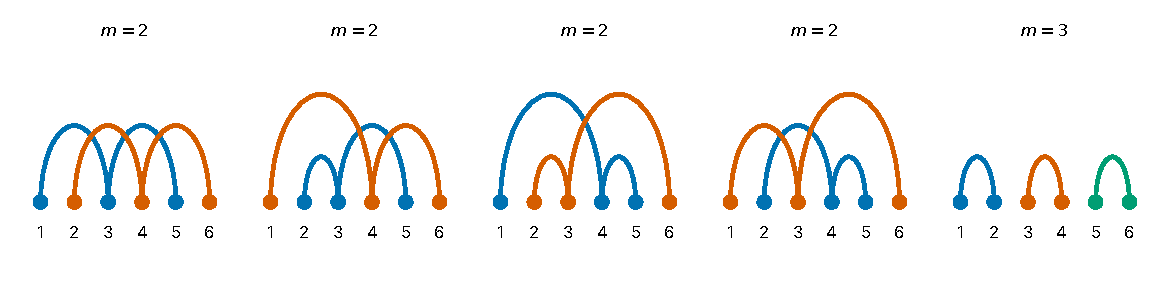
\includegraphics[width=0.95\textwidth]{figures/fig08_two_partitions.pdf}
\caption{The five partitions of the all-ones word of the minimal reduced box with $k=4$, $p=6$ (representative $X=\{8,\dots,13\}\subset\AG(3,2)$): four partitions into two circuits of size~$3$, one into three circuits of size~$2$. \figdesc{exact data from the circuit list; blocks drawn as arcs over the six coordinates.}}\label{fig:twopart}
\end{figure}

\begin{figure}[ht]
\centering
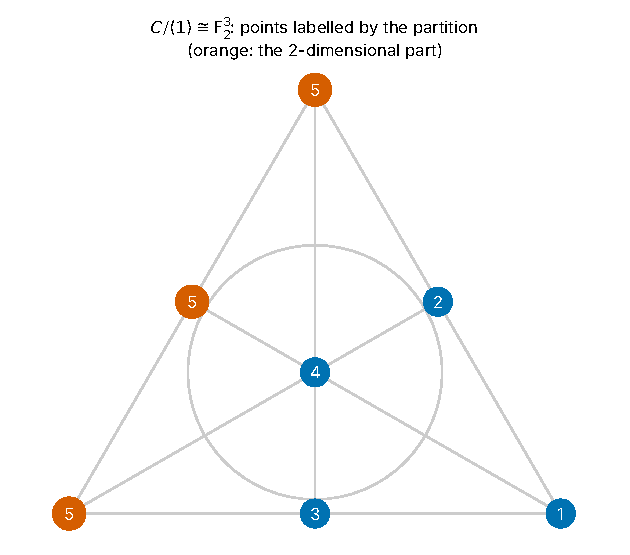
\includegraphics[width=0.8\textwidth]{figures/fig09_vsp_fano.pdf}
\caption{The vector-space partition of $C/\langle\one\rangle\cong\F_2^3$ (the Fano plane) for the same box: four singleton parts (points) and one part of dimension $2$ (a line). \figdesc{points are the seven nonzero cosets of $\langle\one\rangle$, computed exactly; drawing is schematic.}}\label{fig:fano}
\end{figure}

%% -------------------------------------------------------------------
\section{The counting identity}\label{sec:counting}

\begin{theorem}[Counting identity; \gid{G11-L5}]\label{thm:counting}
For a minimal non-embedded box of nullity $k$,
\[
\sum_{P\in\Part}\bigl(2^{m_P}-2\bigr)=2^k-2,\qquad\text{equivalently}\qquad\sum_{P\in\Part}\bigl(2^{m_P-1}-1\bigr)=2^{k-1}-1 .
\]
In terms of $n_m=\#\{P: m_P=m\}$: $\sum_{m\ge2}n_m(2^m-2)=2^k-2$.
\end{theorem}

\begin{proof}
Each $V_P\setminus\{0,\one\}$ has $2^{m_P}-2$ elements and these sets partition $C\setminus\{0,\one\}$ (Theorem~\ref{thm:vsp}), which has $2^k-2$ elements.
\end{proof}

\begin{corollary}\label{cor:counting-consequences}
(a)~$n_2\le2^{k-1}-1$, with equality iff all partitions of $\one$ have exactly two blocks. (b)~$\beta=|\Part|\le 2^{k-1}-1$. (c)~If $n_m=0$ for all $m\ge4$ then $2n_2+6n_3=2^k-2$.
\end{corollary}

\begin{proof}
Immediate from $2^m-2\ge2$ for $m\ge2$ and Theorem~\ref{thm:counting}.
\end{proof}

\begin{example}[Checks]\label{ex:counting}
$E_4$ ($k=3$): $3\cdot(4-2)=6=2^3-2$. The minimal reduced box with $k=4,p=6$: $4\cdot2+1\cdot6=14=2^4-2$. $\AG(3,2)$ ($k=4$, $p=8$): $7\cdot2=14$. The classes with $k=5$, $p=10$ and $n_2=12$, $n_3=1$: $12\cdot2+6=30=2^5-2$. All $231$ minimal reduced classes with $k\le6$ satisfy the identity (exact check; Appendix~\ref{app:repro}).
\end{example}

\begin{figure}[ht]
\centering
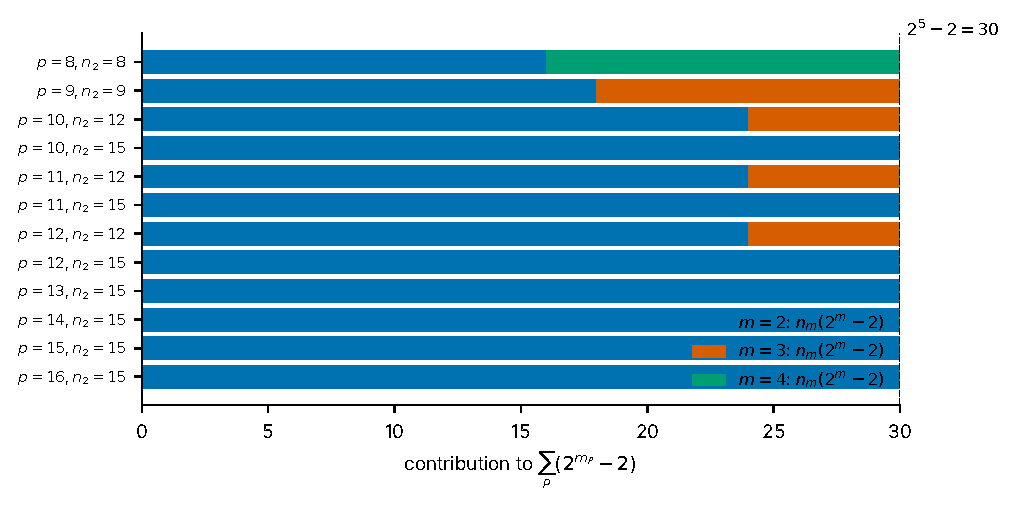
\includegraphics[width=0.95\textwidth]{figures/fig10_counting_identity.pdf}
\caption{The counting identity for the twelve minimal reduced classes with $k=5$: stacked contributions $n_m(2^m-2)$ to the total $2^k-2=30$. \figdesc{exact from the classification of Section~\ref{sec:classify}.}}\label{fig:counting}
\end{figure}

%% -------------------------------------------------------------------
\section{The second-moment (Parseval) identity}\label{sec:parseval}

For a word $w$ write $|w|=\wt(w)$.

\begin{lemma}[Second moment of the weight]\label{lem:moment}
Let $C$ be a reduced code of nullity $k$ and length $p$ (no dead coordinates, no two series-equivalent coordinates). Then
\[
\sum_{w\in C}|w|^2=2^{k-2}\,p\,(p+1).
\]
\end{lemma}

\begin{proof}
$|w|^2=\sum_{i,j}w_iw_j$. For each coordinate $i$, $\#\{w: w_i=1\}=2^{k-1}$ because the $i$th coordinate functional is nonzero on $C$. For $i\ne j$ the pair of functionals $(w\mapsto w_i,\,w\mapsto w_j)$ on $C$ is linearly independent (the coordinates are neither dead nor series-equivalent: a relation $w_i=w_j$ for all $w$ or $w_i=0$ for all $w$ is excluded), so $\#\{w:w_i=w_j=1\}=2^{k-2}$. Therefore $\sum_w|w|^2=p\,2^{k-1}+p(p-1)2^{k-2}=2^{k-2}p(p+1)$.
\end{proof}

(In coding-theoretic language the hypothesis says the dual code has minimum distance at least $3$, i.e.\ $C$ is an orthogonal array of strength~$2$; the formula is the second moment in the MacWilliams framework \cite{MacWilliamsSloane1977}.)

\begin{lemma}[Block expansion]\label{lem:block}
Let $P$ be a partition of $[p]$ into blocks of sizes $b_1,\dots,b_m$ and put $S_P=\sum_jb_j^2$. Then
\[
\sum_{w\in V_P}|w|^2=2^{m-2}\bigl(S_P+p^2\bigr).
\]
\end{lemma}

\begin{proof}
A word of $V_P$ is the union of the blocks indexed by $J\subseteq[m]$, with weight $\sum_{j\in J}b_j$. Summing over all $J$: each $b_j^2$ appears in $2^{m-1}$ subsets, each cross term $b_jb_l$ ($j\ne l$, counted twice in the square) in $2^{m-2}$, so $\sum_J(\sum_{j\in J}b_j)^2=2^{m-1}S_P+2^{m-2}(p^2-S_P)=2^{m-2}(S_P+p^2)$.
\end{proof}

\begin{theorem}[Parseval identity; \gid{G11-L5b}]\label{thm:parseval}
For a minimal non-embedded box (reduced, length $p$, nullity $k$),
\[
\sum_{P\in\Part}\bigl(2^{m_P}S_P-2p^2\bigr)=p\,(2^k-2p),
\]
where $S_P=\sum_{B\in P}|B|^2$. For a partition $P=\{B_1,B_2\}$ into two blocks the summand is $2(|B_1|-|B_2|)^2\ge0$.
\end{theorem}

\begin{proof}
Partition $C=\{0\}\sqcup\{\one\}\sqcup\bigsqcup_P(V_P\setminus\{0,\one\})$ (Theorem~\ref{thm:vsp}). The word $0$ has weight $0$ and $\one$ has weight $p$. By Lemmas~\ref{lem:moment} and~\ref{lem:block},
\[
2^{k-2}p(p+1)=p^2+\sum_P\Bigl[2^{m_P-2}(S_P+p^2)-p^2\Bigr].
\]
Multiply by $4$ and use $\sum_P 2^{m_P}=2^k-2+2\beta$ (Theorem~\ref{thm:counting}, with $\beta=|\Part|$):
\[
2^kp(p+1)=4p^2+\sum_P2^{m_P}S_P+p^2(2^k-2+2\beta)-4\beta p^2,
\]
that is, $\sum_P2^{m_P}S_P=2^kp(p+1)-4p^2-p^2(2^k-2)+2\beta p^2=2^kp-2p^2+2\beta p^2$. Subtracting $2\beta p^2$ gives $\sum_P(2^{m_P}S_P-2p^2)=2^kp-2p^2=p(2^k-2p)$. For $m=2$, $4(b_1^2+b_2^2)-2(b_1+b_2)^2=2(b_1-b_2)^2$.
\end{proof}

\src{\gid{G11-L5b}, GEO-I v011 \texttt{MATHEMATICS.md} \S1.4 (\PROVED). Re-derived here from Lemmas~\ref{lem:moment}--\ref{lem:block}; the identity was verified exactly for all $231$ classified classes with $k\le6$ (Appendix~\ref{app:repro}).}

\begin{example}[Checks]\label{ex:parseval}
$E_4$: $p=4$, $k=3$, three partitions with blocks $(2,2)$, so $S_P=8$ and each summand is $4\cdot8-32=0$; the right side is $4\,(8-8)=0$. For the $k=4$, $p=6$ box: the three-block partition has $S=12$ and summand $8\cdot12-72=24$, the right side is $6\,(16-12)=24$, so the four two-block summands $2(b_1-b_2)^2$ sum to $0$ and each two-block partition has two blocks of size~$3$. $\AG(k-1,2)$: all $2^{k-1}-1$ partitions have blocks of size $p/2$, every summand vanishes, and the right side $p(2^k-2p)=0$ because $p=2^{k-1}$.
\end{example}

\begin{remark}[Fourier-analytic reading]\label{rem:fourier}
The weight enumerator of $C$ is the Fourier transform (over the group $\F_2^k$ of functionals) of the indicator of the point set $X$, and Lemma~\ref{lem:moment} is its second moment \cite{Terras1999,ODonnell2014}. The theorem says that this second moment is also the sum of the second moments of the pieces $V_P$ of the vector-space partition, each of which is computable from the block sizes alone. This is what makes the partition data so rigid.
\end{remark}

%% -------------------------------------------------------------------
\section{Quantitative inequalities}\label{sec:ineq}

Put, for $P\in\Part$ with $m=m_P$ blocks,
\[
t_P=2^{m}S_P-2p^2-p\,(2^{m}-2).
\]
Subtracting $p$ times the counting identity from the Parseval identity gives
\begin{equation}\label{eq:tsum}
\sum_{P\in\Part}t_P=p(2^k-2p)-p(2^k-2)=-2p(p-1).
\end{equation}

\begin{lemma}[Cauchy--Schwarz]\label{lem:CS}
$S_P\ge p^2/m_P$, with equality iff all blocks of $P$ have the same size $p/m_P$.
\end{lemma}

\begin{lemma}[Block bound]\label{lem:mbound}
$2\le m_P\le p/2$ for every $P\in\Part$.
\end{lemma}

\begin{proof}
Every block has size $\ge2$ (Corollary~\ref{cor:minprops}) and the sizes add to $p$.
\end{proof}

\begin{lemma}[Two-block terms]\label{lem:t2}
If $m_P=2$ then $t_P=2(|B_1|-|B_2|)^2-2p\ge-2p$, with equality iff $|B_1|=|B_2|$.
\end{lemma}

\begin{lemma}[Threshold inequality]\label{lem:threshold}
For integers $p\ge9$ and $3\le m\le p/2$,
\[
p\Bigl(\frac{2^m}{m}-2\Bigr)\ \ge\ 2^m-2,
\]
with equality if and only if $(p,m)=(9,3)$. For $p\in\{6,7,8\}$ the inequality fails for $m=3$, and it holds strictly for $m=4$, $p=8$.
\end{lemma}

\begin{proof}
Since $2^m/m-2>0$ for $m\ge3$ the inequality is equivalent to $p\ge f(m):=\dfrac{m(2^m-2)}{2^m-2m}$ (the denominator is positive for $m\ge3$). We compute $f(3)=\frac{3\cdot6}{2}=9$, $f(4)=\frac{4\cdot14}{8}=7$, $f(5)=\frac{5\cdot30}{22}=\frac{75}{11}<7$. For $m=3$ the inequality $p\ge9$ holds with equality iff $p=9$. For $m=4$ we have $p\ge8>7$ since $m\le p/2$ gives $p\ge8$. For $m\ge5$ write $f(m)=m+\dfrac{m(2m-2)}{2^m-2m}$; then $f(m)<2m$ is equivalent to $m(2m-2)<m(2^m-2m)$, i.e.\ $2^m>4m-2$, which holds for $m\ge4$ ($16>14$) and propagates by $2^{m+1}=2\cdot2^m>8m-4\ge4(m+1)-2$ for $m\ge1$. Since $p\ge2m>f(m)$ the inequality is strict. For $p\in\{6,7,8\}$ and $m=3$: $p<9=f(3)$, so the inequality fails.
\end{proof}

\begin{table}[ht]
\centering\small
\begin{tabular}{@{}rrrrr@{}}
\toprule
$m$ & $f(m)$ & $\lceil f(m)\rceil$ & $2m$ & range of $p$ where $p\ge f(m)$ and $p\ge2m$ \\
\midrule
$3$ & $9$ & $9$ & $6$ & $p\ge9$\\
$4$ & $7$ & $7$ & $8$ & $p\ge8$\\
$5$ & $75/11\approx6.82$ & $7$ & $10$ & $p\ge10$\\
$6$ & $6\cdot62/52\approx7.15$ & $8$ & $12$ & $p\ge12$\\
$7$ & $7\cdot126/114\approx7.74$ & $8$ & $14$ & $p\ge14$\\
$8$ & $8\cdot254/240\approx8.47$ & $9$ & $16$ & $p\ge16$\\
\bottomrule
\end{tabular}
\caption{The threshold function $f(m)=m(2^m-2)/(2^m-2m)$. For every $m\ge4$ one has $f(m)<2m$, so the constraint $m\le p/2$ already forces $p>f(m)$. Only $m=3$ imposes a nontrivial lower bound, $p\ge9$.}\label{tab:threshold}
\end{table}

\begin{corollary}[Sign of the higher terms]\label{cor:tpos}
If $p\ge9$ then $t_P\ge0$ for every $P\in\Part$ with $m_P\ge3$, and $t_P>0$ unless $(p,m_P)=(9,3)$ and all three blocks have size $3$.
\end{corollary}

\begin{proof}
By Lemma~\ref{lem:CS}, $t_P\ge p\bigl[p(2^m/m-2)-(2^m-2)\bigr]$ with $m=m_P\le p/2$; apply Lemma~\ref{lem:threshold}. Equality forces $(p,m)=(9,3)$ and equality in Cauchy--Schwarz.
\end{proof}

\begin{remark}[The exceptional finite range]\label{rem:exceptional}
For $p\le8$ the bound of Corollary~\ref{cor:tpos} fails only for $m=3$ (which requires $p\ge6$), and only for $p=6,7,8$. There the Cauchy--Schwarz bound gives $t_P\ge p\bigl[\tfrac23p-6\bigr]$, i.e.\ $-12$, $-\tfrac{28}{3}$ and $-\tfrac{16}{3}$ for $p=6,7,8$ (Appendix~\ref{app:I}). With such negative terms permitted, the identities and inequalities alone do not exclude a profile with at most one two-block partition: the supplementary scan \gid{G11-V1} of the source reports, for $k=5$, one numerically feasible profile with $p=6$ which no code realizes (our enumeration in Table~\ref{tab:smallp} finds no minimal box at $(k,p)=(5,6)$). The cases $p\le8$ are therefore treated by exhaustive enumeration (Section~\ref{sec:W2}).
\end{remark}

%% -------------------------------------------------------------------
\section{At least \texorpdfstring{$p-1$}{p-1} two-block partitions}\label{sec:n2}

\begin{theorem}[$n_2\ge p-1$; \gid{G11-L6}]\label{thm:L6}
Let $C$ be a minimal non-embedded box (reduced, length $p\ge9$, nullity $k$). Then
\[
n_2\ \ge\ p-1 .
\]
If $p\ge10$ then equality holds if and only if $X=\AG(k-1,2)$ (so $p=2^{k-1}$ and $C=\mathrm{RM}(1,k-1)$). If $p=9$ equality is impossible, so $n_2\ge9$.
\end{theorem}

\begin{proof}
By~\eqref{eq:tsum}, $-2p(p-1)=\sum_Pt_P$. Split into two-block and higher partitions. Lemma~\ref{lem:t2} gives $\sum_{m_P=2}t_P\ge-2p\,n_2$ and Corollary~\ref{cor:tpos} gives $\sum_{m_P\ge3}t_P\ge0$. Hence $-2p(p-1)\ge-2pn_2$, i.e.\ $n_2\ge p-1$.

\emph{Equality.} If $n_2=p-1$ all inequalities are tight: every two-block partition is balanced (blocks of size $p/2$) and $\sum_{m_P\ge3}t_P=0$. For $p\ge10$ Corollary~\ref{cor:tpos} gives $t_P>0$ for every $m_P\ge3$, so there is no partition with $m_P\ge3$. Then the counting identity reads $2n_2=2^k-2$, so $p-1=n_2=2^{k-1}-1$ and $p=2^{k-1}=|H|$: $X=H=\AG(k-1,2)$. Conversely $X=\AG(k-1,2)$ has $n_2=p-1$ by Proposition~\ref{prop:RM}. For $p=9$, equality would force every $m_P\ge3$ partition to have $m_P=3$ with blocks $3,3,3$ (the exceptional case of Corollary~\ref{cor:tpos}) and so $2\cdot8+6n_3=2^k-2$, i.e.\ $2^k=18+6n_3$ is divisible by $3$, which is absurd.
\end{proof}

\src{\gid{G11-L6}, GEO-I v011 \texttt{MATHEMATICS.md} \S1.5 (\PROVED+\CHECKED); sharpness \gid{G11-K1} (\CHECKED in the source). The characterisation of the equality case for $p\ge10$ and the impossibility for $p=9$ are made explicit here (new here). The bound was confirmed on all $231$ classified classes and on $19\,373$ labelled minimal subsets for $k=5$ (min $n_2=8$).}

\begin{proposition}[The Reed--Muller family]\label{prop:RM}
For $k\ge3$ let $X=\AG(k-1,2)$ (all $p=2^{k-1}$ points of $H$) and $C=\mathrm{RM}(1,k-1)$. Then the circuits are the $2^k-2$ words of weight $p/2$; the partitions of $\one$ are the $2^{k-1}-1$ pairs $\{w,\one\oplus w\}$; $n_2=p-1$; $C$ is minimal non-embedded; $\rmin=3$.
\end{proposition}

\begin{proof}
The words are the affine functions on $\F_2^{k-1}$: $0$, $\one$ and $2^k-2$ words of weight $p/2$. Distinct nonzero words of equal weight are not nested, and every word other than $0,\one$ is nonconstant and has weight $p/2$, so the circuits are exactly the $2^k-2$ words of weight $p/2$ (the word $\one$ contains each, so is not a circuit). Two disjoint circuits have total weight $p$, hence are complementary: the partitions of $\one$ are the pairs $\{w,\one\oplus w\}$, of which there are $(2^k-2)/2$. For $k\ge3$ this is $\ge3$, so $C$ is non-embedded by Theorem~\ref{thm:E1}. Shortening at a coordinate $i$: the circuits avoiding $i$ are the $w$ with $w_i=0$; two disjoint ones are complementary, so one of them contains $i$: contradiction. Hence no set is partitioned into two or more circuits in $C_{(i)}$, every set has at most one partition, and $C_{(i)}$ is embedded. Rank three follows from Theorem~\ref{thm:L5}.
\end{proof}

\src{\gid{G8-T3c}, GEO-I v008 \texttt{MINIMAL\_RANK.md} (\PROVED, \CHECKED for $k=3,4,5$); re-proved above by a direct argument.}

\begin{figure}[ht]
\centering
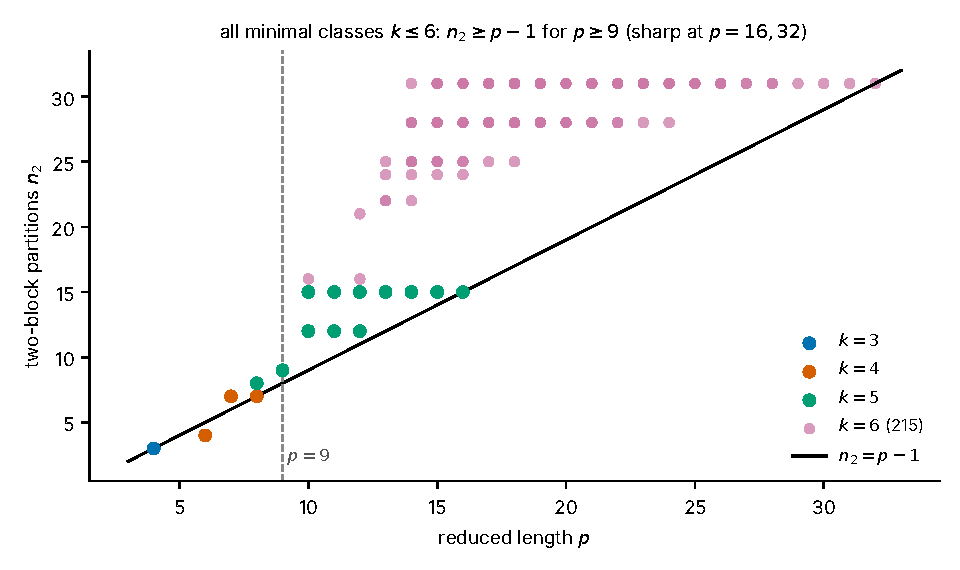
\includegraphics[width=0.95\textwidth]{figures/fig11_n2_bound.pdf}
\caption{The number $n_2$ of two-block partitions against the reduced length $p$ for all minimal classes with $k=3,\dots,6$ ($231$ classes), with the line $n_2=p-1$ and the threshold $p=9$. Points on the line are the Reed--Muller supports $p=4,8,16,32$. \figdesc{exact data; for $k=6$ from the source-reported list of $215$ representatives recomputed with the independent engine.}}\label{fig:n2}
\end{figure}

%% -------------------------------------------------------------------
\section{W2 universality}\label{sec:W2}

The inequality of Section~\ref{sec:n2} settles $p\ge9$. For $p\le8$ we use a normal form that reduces the problem to a very small enumeration.

\begin{lemma}[Simplex normal form]\label{lem:simplex}
Let $X\subseteq H\cong\AG(k-1,2)$ be a spanning subset with $|X|=p$. Then $X$ is $\AGL(k-1,2)$-equivalent to a set
\[
\{e_1,\dots,e_k\}\cup R,\qquad R\subseteq O_k,\ |R|=p-k,
\]
where, in suitable coordinates, $H$ is the set of odd-weight vectors of $\F_2^k$ and $O_k$ is the set of odd-weight vectors of weight $\ge3$.
\end{lemma}

\begin{proof}
$X$ spans $\F_2^k$, so it contains a basis $b_1,\dots,b_k$. Since $f_0(b_i)=1$ for all $i$, in the basis $(b_i)$ the functional $f_0$ is $(1,\dots,1)$, so $H$ is the set of odd-weight vectors and $b_i=e_i$. The change of basis fixes $f_0$, hence induces an element of $\AGL(k-1,2)$ (Section~\ref{sec:affine}). The remaining points of $X$ are odd-weight vectors different from $e_i$, i.e.\ of weight $\ge3$.
\end{proof}

\begin{proposition}[Finite check for $p\le8$]\label{prop:small}
For every pair $(k,p)$ with $3\le k<p\le8$ let $\mathcal N_{k,p}$ be the set of subsets $R\subseteq O_k$ with $|R|=p-k$ (so $\binom{|O_k|}{p-k}$ candidates). For each candidate the reduced box $\{e_1,\dots,e_k\}\cup R$ was tested for non-embeddedness (Theorem~\ref{thm:E1}, direct enumeration of circuit partitions), minimality (non-embeddedness of every shortening), and $n_2$ (the number of partitions of $\one$ into two circuits). The results are in Table~\ref{tab:smallp}: minimal boxes occur only for $(k,p)\in\{(3,4),(4,6),(4,7),(4,8),(5,8)\}$ and they have $n_2\ge3$.
\end{proposition}

\begin{table}[ht]
\centering\small
\begin{tabular}{@{}rrrrrr@{}}
\toprule
$p$ & $k$ & candidates & non-embedded & minimal & $\min n_2$ over minimal\\
\midrule
\smallptablebody
\bottomrule
\end{tabular}
\caption{The finite enumeration for $p\le8$ (Proposition~\ref{prop:small}). ``Candidates'' counts the sets $R\subseteq O_k$ of size $p-k$. All candidates are non-embedded. Minimal boxes with $p\le8$ exist only for the pairs $(k,p)=(3,4),(4,6),(4,7),(4,8),(5,8)$; for $(k,p)=(5,8)$ ten of the $165$ candidates are minimal.}\label{tab:smallp}
\end{table}

\src{New here as a self-contained route (Appendix~\ref{app:K}); \texttt{scripts/small\_p.py}, own code. The source proves W2 for $p\le8$ via the classification through nullity $6$ (\gid{G11-T3}, \texttt{MATHEMATICS.md} \S1.7) and the exclusion of $(k,p)=(7,8)$ (\gid{G11-L6b}). Both routes agree. Status of Proposition~\ref{prop:small}: \PROVED+\CHECKED (exhaustive, complete, $655$ candidates in total; no hand proof).}

\begin{figure}[ht]
\centering
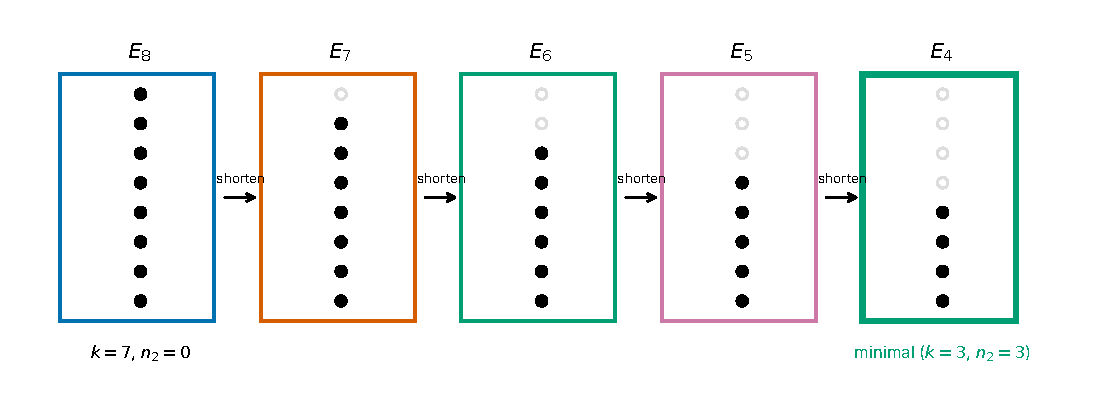
\includegraphics[width=0.95\textwidth]{figures/fig13_E8_nonminimal.pdf}
\caption{The case $(k,p)=(7,8)$: $C=E_8$ with its $28$ weight-two circuits and $105$ perfect matchings of the coordinates, but no partition of $\one$ into two circuits. $E_8$ is not minimal because shortening gives $E_7$, then $E_6,E_5,E_4$, which is the minimal sub-box on four coordinates. \figdesc{schematic chain of shortenings; the sub-box $E_4$ sits on any four of the eight coordinates.}}\label{fig:E8}
\end{figure}

\begin{theorem}[W2 universality; \gid{G11-T3}]\label{thm:W2}
Every minimal non-embedded box satisfies W2: the all-ones word has at least two partitions into exactly two circuits, i.e.\ $n_2\ge2$. More precisely, if $p\ge9$ then $n_2\ge p-1\ge8$, and if $p\le8$ then $n_2\ge3$.
\end{theorem}

\begin{proof}
If $p\ge9$, Theorem~\ref{thm:L6}. If $p\le8$, the reduced code is a spanning subset of $\AG(k-1,2)$ with $k+1\le p\le8$ points (Theorem~\ref{thm:affine}), hence equivalent to one of the candidates of Proposition~\ref{prop:small} by Lemma~\ref{lem:simplex}; by Table~\ref{tab:smallp} every minimal one has $n_2\ge3$. The cases with $p=k+1$ are consistent with this: they are the even-weight codes $E_p$, minimal only for $p=4$ (Proposition~\ref{prop:Emin}); in particular the case $(k,p)=(7,8)$ ($C=E_8$, with $28$ circuits of weight two, $105$ perfect matchings and $n_2=0$) is not minimal.
\end{proof}

\src{\gid{G11-T3} (= \gid{G10-C1} = \gid{G11-C2}), GEO-I v011 \texttt{MATHEMATICS.md} \S1.7 (\PROVED+\CHECKED). The part for $p\ge9$ is proved in the text without any enumeration. The part for $p\le8$ rests on the exhaustive enumeration above (and, in the source, on the classification for $k\le6$ and \gid{G11-L6b}).}

%% -------------------------------------------------------------------
\section{The main theorem: universal rank three}\label{sec:main}

\begin{theorem}[Universal minimum witness rank; \gid{G11-T4}]\label{thm:rank3}
For every non-embedded box $C$ of the frozen binary $0/1$ Graver-cell model, of arbitrary length $n$, nullity $k$ and parity matrix (zero columns included),
\[
\rmin(C)=3 .
\]
The value $3$ is attained by a collision of two cells of dimension~$2$ obtained from two two-circuit partitions of $\one$ in a minimal sub-box.
\end{theorem}

\begin{proof}
Theorem~\ref{thm:W2} shows that every minimal non-embedded box satisfies W2. Theorem~\ref{thm:C1p} (descent to a minimal sub-box, Theorem~\ref{thm:L5} for the upper bound, Lemma~\ref{lem:LOW} for the lower bound) yields $\rmin(C)=3$.
\end{proof}

\src{\gid{G11-T4}, GEO-I v011 \texttt{RANK\_UNIVERSAL.md} (\PROVED). All steps are proved in this paper except the finite enumeration of Proposition~\ref{prop:small}.}

\begin{corollary}[No minimal box of rank four]\label{cor:no4}
No minimal non-embedded box has $\rmin\ge4$. Consequently the conjecture \gid{G10-C2} (``a minimal box with $\rmin=4$ exists'') is false in the frozen model, and the statement ``$\rmin\ge4$ implies nullity $\ge7$'' (\gid{G10-T4}) is vacuous.
\end{corollary}

\src{\gid{G11-C3}: status \textsc{false} for \gid{G10-C2}, GEO-I v011 \texttt{RANK\_UNIVERSAL.md}.}

\begin{remark}[What the theorem does not say]\label{rem:notalg}
(i)~Individual collisions can have large rank (Remark~\ref{rem:individual}). (ii)~The theorem is about the \emph{existence} of a rank-three collision in every non-embedded box; it gives no bound on how hard it is to \emph{find} one. (iii)~The theorem is for the frozen binary model only. (iv)~The proof of W2 for $p\le8$ is by a complete but computer-executed enumeration; the proof for $p\ge9$ is a hand proof.
\end{remark}

\begin{figure}[ht]
\centering
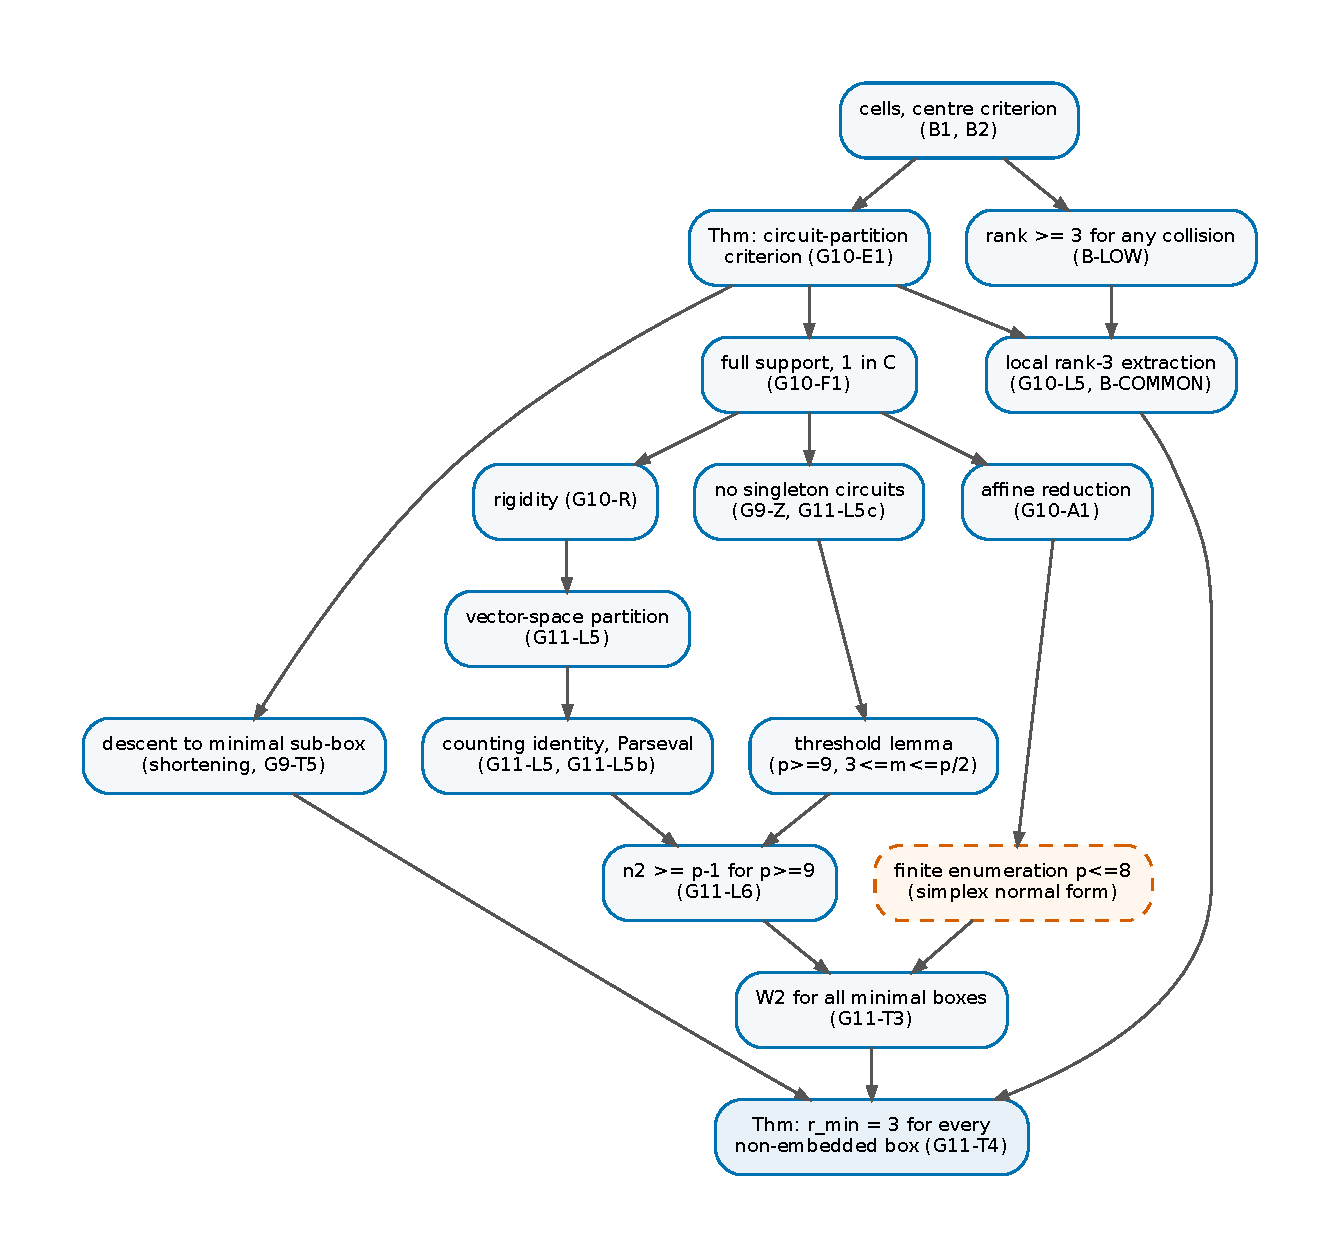
\includegraphics[width=0.95\textwidth]{figures/fig14_dependencies.pdf}
\caption{Dependency diagram of the proof. Arrows point from a result to the results that use it. Dashed boxes mark the finite enumeration ($p\le8$) and the supplementary source-reported material (nullity-$6$ classification), which is not used in the proof of the main theorem. \figdesc{generated by \texttt{scripts/figs.py}.}}\label{fig:deps}
\end{figure}

%% ===================================================================
%% PART IV
%% ===================================================================
\part{Examples, classification and consequences}

%% -------------------------------------------------------------------
\section{The explicit rank-three obstruction}\label{sec:E4}

\subsection{The even-weight code of length four}

Let $C=E_4=\{w\in\F_2^4:\ \wt(w)\ \text{even}\}$, the kernel of $M=(1\,1\,1\,1)$; $k=3$. We write words by their supports, e.g.\ $13$ for $\{1,3\}$.

\paragraph{Circuits.} The six weight-two words $12,13,14,23,24,34$ (Proposition~\ref{prop:Emin}); $1234$ is not a circuit. Pairs of disjoint circuits: $\{12,34\}$, $\{13,24\}$, $\{14,23\}$. So $\Part=\{P_1,P_2,P_3\}$ with $P_1=\{12,34\}$, $P_2=\{13,24\}$, $P_3=\{14,23\}$, and $n_2=3$, $m_P=2$ for all three. The counting identity reads $3\cdot(2^2-2)=6=2^3-2$.

\paragraph{Cells.} The fibre is $F=\{12,13,14,23,24,34,1234\}$ (seven points). A direct enumeration from Definition~\ref{def:cell} gives $7$ vertices, $18$ edges ($6$ circuits $\times$ $3$ admissible cosets) and exactly $3$ two-dimensional cells:
\begin{align*}
Z_A&=Z(\{12,34\},13)\quad\text{vertices }13,\,14,\,23,\,24,\\
Z_B&=Z(\{13,24\},12)\quad\text{vertices }12,\,14,\,23,\,34,\\
Z_C&=Z(\{14,23\},12)\quad\text{vertices }12,\,13,\,24,\,34.
\end{align*}
Their unions are all $\{1,2,3,4\}$, there is nothing outside the union, and the three centres are $(\tfrac12,\tfrac12,\tfrac12,\tfrac12)$ (Theorem~\ref{thm:centre}). Hence all three pairs collide. The cells $Z_A,Z_B$ share the diagonal with endpoints $14$ and $23$; $Z_A,Z_C$ share $13,24$; $Z_B,Z_C$ share $12,34$. The cell structure is the three equatorial squares of the octahedron with vertices $12,13,14,23,24,34$, together with the vertex $1234$ and edges to it (Figure~\ref{fig:octa}).

\paragraph{The rank.} With the common base point $x=14$ (not in $\spn P_1=\{0,12,34,1234\}$ nor in $\spn P_2=\{0,13,24,1234\}$), $s=(1-2x_i)_i=(-1,1,1,-1)$ and
\[
g_1=(-1,1,0,0),\ g_2=(0,0,1,-1);\qquad h_1=(-1,0,1,0),\ h_2=(0,1,0,-1).
\]
Then $g_1+g_2=(-1,1,1,-1)=h_1+h_2$. The vectors $g_1,g_2,h_1$ are independent: a relation $ag_1+bg_2+ch_1=0$ gives from coordinate~$2$ that $a=0$, from coordinate~$4$ that $b=0$ and then $c=0$. So the witness rank is exactly $3$. Because $r=t=2$, the witness space has dimension $3=r+t-1$. By Lemma~\ref{lem:LOW} no collision of $E_4$ has smaller rank; by Theorem~\ref{thm:rank3} the same is true of every non-embedded box.

\begin{remark}[Geometry of the witness]
The three planes in $\R^4$ spanned by $Z_A,Z_B,Z_C$ lie in the common affine hyperplane $\sum x_i=2$, which is $3$-dimensional. In that $\R^3$ the octahedron is a genuine picture: two equatorial squares meet along a diagonal and a third square passes through the common centre. The collision is thus a ``crossing of two planes in a $3$-space'', the simplest possible crossing.
\end{remark}

\subsection{Minimality and uniqueness}

\begin{proposition}\label{prop:unique-k3}
$E_4$ is minimal (Proposition~\ref{prop:Emin}). Every minimal non-embedded box of nullity $3$ is a blow-up of $E_4$ (that is, $p=4$ and $X=\AG(2,2)$).
\end{proposition}

\begin{proof}
For $k=3$ the affine space $H=\AG(2,2)$ has four points, so $p\le4$, and $p\ge k+1=4$ gives $X=H$; the code is $\mathrm{RM}(1,2)=E_4$.
\end{proof}

\subsection{Higher nullity}

\paragraph{Reed--Muller family.} By Proposition~\ref{prop:RM}, for every $k\ge3$ the box $\mathrm{RM}(1,k-1)$ of length $2^{k-1}$ is minimal non-embedded, with $2^{k-1}-1$ two-circuit partitions of $\one$ into complementary pairs of weight $p/2$. For $k=4$ ($n=8$): circuits are the $14$ words of weight $4$; the rank-three collision uses any two of the seven partitions. For $k=3$ it is $E_4$.

\paragraph{Blow-ups.} Replacing coordinate $i$ of $E_4$ by $\mu_i\ge1$ copies gives minimal boxes of every length $n\ge4$ and nullity $3$ (Proposition~\ref{prop:series}); all have $\rmin=3$.

\paragraph{Beyond Reed--Muller.} The minimal reduced box with $k=4$, $p=6$ has point set (coordinates $1,\dots,6$)
\[
X=\{1000,1001,1010,1011,1100,1101\}\subset\AG(3,2),
\]
$11$ circuits, and the five partitions of $\one$ shown in Figure~\ref{fig:twopart}: the four two-block partitions $\{135|246\}$, $\{235|146\}$, $\{145|236\}$, $\{245|136\}$ and the three-block partition $\{12|34|56\}$. The identity $4\cdot2+6=14=2^4-2$ holds, as does Parseval's identity (Example~\ref{ex:parseval}). A rank-three collision comes from any two of the four two-block partitions. The class with $k=5$, $p=8$ has two-block partitions (eight of them) and one four-block partition $\{12|34|56|78\}$, with $8\cdot2+14=30$.

\begin{remark}[Individual versus minimum, again]
Exact enumeration shows that the $k=4$, $p=6$ box has $78$ collisions ($66$ between cells of dimensions $(2,2)$ and $12$ between $(2,3)$), of witness rank $3$ ($30$ times) and $4$ ($48$ times); the $k=5$, $p=8$ box has $1596$ collisions ($1540$ of type $(2,2)$ and $56$ of type $(2,4)$) with ranks $3,4,5$ occurring $364,1176,56$ times. The theorem concerns the \emph{minimum}.
\end{remark}

%% -------------------------------------------------------------------
\section{Exact finite classification}\label{sec:classify}

This section reports the classification of minimal reduced boxes for small nullity. It is \emph{not used} in the proof of Theorem~\ref{thm:rank3}; its role is to document the examples, to provide independent evidence for the general theorems, and to record what is known beyond them.

\subsection{What is classified}

By Theorem~\ref{thm:affine} and Proposition~\ref{prop:series}, a minimal non-embedded box is determined, up to coordinate permutation and basis change, by (i)~its nullity $k$, (ii)~a spanning subset $X\subseteq\AG(k-1,2)$ up to $\AGL(k-1,2)$, and (iii)~a multiplicity function $\mu:X\to\Z_{\ge1}$. So classifying minimal boxes of nullity $k$ means classifying the $\AGL(k-1,2)$-orbits of subsets $X$ whose reduced box is minimal non-embedded; call these \emph{minimal classes}.

\subsection{Results}

\begin{table}[ht]
\centering\small
\begin{tabular}{@{}rrrp{6.2cm}@{}}
\toprule
$k$ & minimal classes & $p$ range & status and provenance\\
\midrule
$3$ & $1$ & $4$ & \PROVED+\CHECKED; re-enumerated here\\
$4$ & $3$ & $6,7,8$ & \PROVED+\CHECKED; re-enumerated here ($37$ labelled subsets)\\
$5$ & $12$ & $8,\dots,16$ & \PROVED+\CHECKED; re-enumerated here ($19\,373$ labelled subsets)\\
$6$ & $215$ & $10,\dots,32$ & source-reported (\gid{G10-T4}); the $215$ representatives were re-checked here; completeness not re-derived\\
\bottomrule
\end{tabular}
\caption{Minimal classes of reduced boxes by nullity. ``Re-enumerated'' means that all $2^{2^{k-1}}$ subsets of $\AG(k-1,2)$ were examined with the independent engine of Appendix~\ref{app:repro} (no use of the release code).}\label{tab:classes}
\end{table}

\begin{theorem}[Classification for $k\le5$; \gid{G8-T3b}, \gid{G9-T4}]\label{thm:class35}
The minimal reduced boxes with $k=3,4,5$ form $1$, $3$ and $12$ classes respectively, listed in Table~\ref{tab:classlist}. Each has $n_2\ge p-1$ whenever $p\ge9$ and $n_2\ge3$ always; each satisfies the counting and Parseval identities; all have $\rmin=3$.
\end{theorem}

\begin{proof}
The proof is an exhaustive enumeration. For each $k\in\{3,4,5\}$ every subset $X\subseteq\AG(k-1,2)$ with $|X|\ge k+1$ that spans $\F_2^k$ ($1$, $93$ and $57\,541$ subsets) was tested: non-embeddedness by Theorem~\ref{thm:E1} (enumeration of circuit partitions) and minimality by Definition~\ref{def:minimal} (shortening at each of the $p$ coordinates). The minimal subsets ($1$, $37$, $19\,373$) were grouped into $\AGL(k-1,2)$-orbits by closing under the generators of $\AGL(k-1,2)$ (translations and elementary transvections); the orbit counts are $1$, $3$, $12$, and the orbit sizes $1$; $28,8,1$; $840,4480,6720,448,1680,2688,140,1680,560,120,16,1$ add up to the numbers of subsets above.
\end{proof}

\src{\gid{G8-T3b} (nullity $3,4$, v008 \texttt{MINIMAL\_RANK.md}) and \gid{G9-T4} (nullity $5$, v009 \texttt{MATHEMATICS.md} \S2.2), both \PROVED+\CHECKED in the source. The enumeration here is independent of the release code; counts agree. The classification for nullity $5$ in the source lists $p=8,9,10,10,11,11,12,12,13,14,15,16$; so does Table~\ref{tab:classlist}.}

\begin{table}[ht]
\centering\small
\begin{tabular}{@{}rrrlrr@{}}
\toprule
$k$ & $p$ & $n_2$ & profile $m^{n_m}$ & orbit size & $|\mathrm{Stab}|$\\
\midrule
\classtablebody
\bottomrule
\end{tabular}
\caption{The $16$ minimal classes of nullity $3,4,5$. ``Profile'' lists the number $n_m$ of partitions of $\one$ with $m$ blocks. ``Orbit size'' is the number of labelled subsets of $\AG(k-1,2)$ in the class; $|\mathrm{Stab}|=|\AGL(k-1,2)|/\text{orbit size}$ ($24$, $1344$, $322\,560$ for $k=3,4,5$). Exact output of \texttt{scripts/classify.py}.}\label{tab:classlist}
\end{table}

\paragraph{Burnside counts.} The number of $\AGL(m,2)$-orbits on all subsets of $\AG(m,2)$ (including $\emptyset$) is $5,10,32$ for $m=2,3,4$ (group orders $24,1344,322\,560$; computed here by Burnside's lemma with exhaustively generated groups) and $382$ for $m=5$ (source-reported). For $k=m+1=6$ this gives the source's chain of counts: $381$ non-empty orbits, $350$ spanning, $349$ non-embedded, $215$ minimal.

\begin{theorem}[Nullity six; \gid{G10-T4}, source-reported]\label{thm:class6}
There are $215$ minimal classes of reduced boxes with $k=6$, with $10\le p\le32$ and $16\le n_2\le31$. Every class has W2, rank $3$, satisfies the identities, and $n_2\ge p-1$ when $p\ge9$ holds in all cases.
\end{theorem}

\src{\gid{G10-T4}, GEO-I v010 \texttt{BINARY6.md} (\PROVED+\CHECKED: certificates \texttt{C6\_rank6.json} with the checker \texttt{checker10.py}). \emph{Independent verification here:} the list of $215$ representative supports was read from the certificate file and, with the independent engine, each was confirmed to be a minimal non-embedded reduced box, to satisfy the counting and Parseval identities and $n_2\ge p-1$ ($p\ge9$), and to have the recorded $n_2$; the $215$ supports are pairwise inequivalent under $\AGL(5,2)$ (separated by invariants, with an exhaustive backtracking search for the $8$ pairs sharing invariants). \emph{Not re-derived:} that the list is complete. Distribution of $(p,n_2)$ in Table~\ref{tab:ksix}.}

\begin{table}[ht]
\centering\small
\begin{tabular}{@{}rrrr@{}}
\toprule
$p$ & classes & $\min n_2$ & $\max n_2$\\
\midrule
\ksixtablebody
\bottomrule
\end{tabular}
\caption{Nullity six: the $215$ source-reported classes, recomputed with the independent engine (\texttt{scripts/verify6.py}).}\label{tab:ksix}
\end{table}

\begin{figure}[ht]
\centering
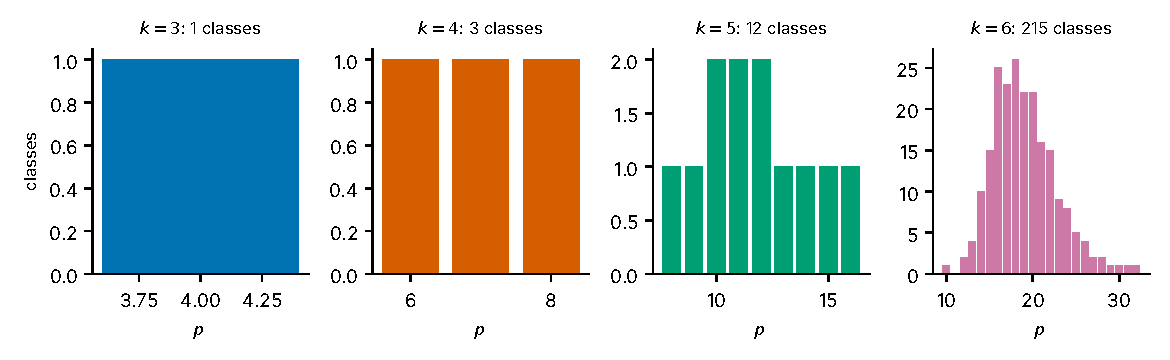
\includegraphics[width=0.95\textwidth]{figures/fig12_classification.pdf}
\caption{Classification summary for $k=3,\dots,6$: number of minimal classes by reduced length $p$. \figdesc{exact counts; $k=6$ from the source-reported list recomputed here.}}\label{fig:classes}
\end{figure}

\subsection{Algorithms and certificates}

\paragraph{Enumeration algorithm ($k\le5$).} For every subset $X$ of $\AG(k-1,2)$ (as a bitmask of the $2^{k-1}$ points): (1)~discard it unless it has rank~$k$ and $p\ge k+1$; (2)~compute all $2^k-1$ nonzero words and their circuits (inclusion-minimal supports); (3)~enumerate all families of pairwise disjoint circuits and record which unions have two partitions (Theorem~\ref{thm:E1}); (4)~for each coordinate $i$ repeat (3) on the circuits avoiding $i$ (Lemma~\ref{lem:shortcirc}); (5)~$X$ is minimal iff (3) finds a double partition and (4) never does. Orbits: union--find over the generators of $\AGL(k-1,2)$.

\paragraph{Certificates.} A \emph{partition certificate} for a point set $X\subseteq\AG(k-1,2)$ consists of the points and two functionals $f\ne g$ whose words are disjoint circuits covering $X$, together with a second such pair; a standalone checker confirms it using only rank computations (source format PARTITION, \texttt{checker11.py}). By Theorems~\ref{thm:E1} and~\ref{thm:L5} a valid certificate proves non-embeddedness with a rank-three collision. It does \emph{not} certify minimality. All $231$ source certificates (every minimal class with $k\le6$) were accepted by the unchanged source checker and, independently, by the engine here.

\paragraph{Separation of roles.} The classification is a table of examples. The universal theorems in Part~III do not depend on it: W2 for $p\ge9$ is proved by inequality, W2 for $p\le8$ by a different small enumeration (Section~\ref{sec:W2}), and Theorem~\ref{thm:rank3} follows.

\subsection{Historical statuses}

Several statements recorded in the release series were later settled; their current status is recorded here for completeness (details in Appendix~\ref{app:crosswalk}): \gid{G8-C3} (full support of minimal boxes) was open in v008--v009 and is proved as Theorem~\ref{thm:F1}; \gid{G10-C1} (universal $\rmin=3$) was open in v010 and is Theorem~\ref{thm:rank3}; \gid{G10-C2} (existence of a rank-four minimal box) is \textsc{false} (Corollary~\ref{cor:no4}); the v010 implication ``$\rmin\ge4$ requires nullity $\ge7$'' is vacuous.

\begin{question}[Spanning sets]\label{q:spanning}
Is the box of every spanning subset $X\subseteq\AG(k-1,2)$ with $|X|\ge k+1$ non-embedded? This holds for $k\le5$ in the exhaustive enumeration here, for $k=6$ in the source counts ($350$ spanning orbits, $349$ non-embedded; the one exceptional orbit is presumably the simplex $p=k$, for which $C=\F_2^k$ is embedded, but we have not checked this against the source enumeration), and in all of $540$ random samples with $k\in\{6,7,8\}$, $p-k\in\{2,3,4\}$ tested here. It is not proved.
\end{question}

%% -------------------------------------------------------------------
\section{Implications}\label{sec:implications}

\subsection{Uniform obstruction dimension}

Theorem~\ref{thm:rank3} says that the \emph{obstruction to embeddedness has a uniform local size}: every non-embedded box, of any length $n$ and nullity $k$, contains a pair of $2$-dimensional cells in a common $3$-dimensional affine subspace whose relative interiors cross at their centres. In geometric language: non-embedding never needs a configuration of higher dimension than the crossing of two planes in $3$-space. The ambient dimension $n$ may be arbitrarily large, and $\spn$ of all cells may be $n$-dimensional, but the obstruction is already visible in dimension three.

\begin{corollary}[A short certificate]\label{cor:cert}
A box $C$ is non-embedded if and only if it contains a word $a$ with two distinct decompositions $a=b_1\sqcup b_2=c_1\sqcup c_2$ into two disjoint circuits.
\end{corollary}

\begin{proof}
($\Leftarrow$)~Theorem~\ref{thm:L5}. ($\Rightarrow$)~By Proposition~\ref{prop:descent} and Theorem~\ref{thm:W2} there is a minimal sub-box $C_{(I)}$ with two two-circuit partitions of its all-ones word; their circuits are circuits of $C$ (Lemma~\ref{lem:shortcirc}), and $a=\one_{[n]\setminus I}$ is a word of $C$ with two decompositions.
\end{proof}

\subsection{Rigidity, finite affine structure, partition universality}

\emph{Rigidity.} In a minimal box the circuit structure is determined by a single failure of unique decomposition (Theorem~\ref{thm:rigid}); the number of cells at the centre is $\sum_P(2^{k-m_P}-1)$ (Proposition~\ref{prop:centre-count}); for example $E_4$ has $3$, the $k=4$, $p=6$ box has $13$, $\AG(3,2)$ has $21$, the $k=5$ classes have $57,69,87,105$ for $p=8,9,10,10$ (verified by direct enumeration).

\emph{Finite affine structure.} Minimal boxes are exactly (up to blow-up) the subsets $X\subseteq\AG(k-1,2)$ whose code has the rigidity property of Proposition~\ref{prop:rigid-char}. The problem of classifying all minimal boxes becomes the problem of classifying certain subsets of affine spaces over $\F_2$ up to the affine group.

\emph{Partition universality.} Every minimal box carries a vector-space partition of $\F_2^{k-1}$ built from its circuit partitions, satisfying the counting identity and the Parseval identity; at least $p-1$ of its parts (for $p\ge9$) are one-dimensional.

\subsection{Local witness versus global complexity}

\begin{remark}[What rank three does and does not give]\label{rem:algo}
Corollary~\ref{cor:cert} gives a certificate of non-embeddedness of size $O(n)$ (five subsets of $[n]$): the verification that $b_1,b_2,c_1,c_2$ are circuits of $C$ summing to the same word requires only rank computations of column submatrices of $M$ (a set $T$ is a circuit iff the columns of $M$ indexed by $T$ have a one-dimensional kernel spanned by $\one_T$). So non-embeddedness has polynomially checkable certificates in the binary-matrix encoding. This does \textbf{not} yield a polynomial-time \emph{algorithm}: the theorem asserts the existence of such a word but not how to find it, and the number of candidates for $a$ is exponential in $n$. We make no claim about the computational complexity of deciding embeddedness; and ``bounded witness rank'' must not be read as ``efficient detection''. The size of the local witness is uniformly $3$; the cost of locating it is unaddressed.
\end{remark}

\subsection{Consequences for the arithmetic model}

Within the arithmetic setting of the GEO-I series the binary boxes arise as the $0/1$ slices of congruence lattices. The theorem implies that, whenever a binary relation lattice (for a given set of active primes and parity configuration) has an exceptional cell overlap, that overlap already occurs in a $3$-dimensional exponent subspace and is generated by exactly two pairs of $2$-dimensional moves. Whether a particular arithmetic fibre is of this binary type is a separate question (Remark~\ref{rem:realize}), which this paper does not address.

%% ===================================================================
%% PART V
%% ===================================================================
\part{Relation to established mathematics, provenance, and open questions}

%% -------------------------------------------------------------------
\section{Relations to established mathematics}\label{sec:literature}

This section compares the objects and results of the paper with standard notions and theorems in neighbouring areas. It is a comparison of definitions and statements, not a survey of the literature, and \emph{no claim of novelty or priority is made}.

\paragraph{What was read, and how.} The following sources were read in full text (as retrieved on the date of the manuscript): Heden's survey of vector-space partitions \cite{Heden2012}; Kurz's paper on Heden's tail bound \cite{KurzTail} (for the exact statement of Heden's theorem); Kurz's classification of vector-space partitions of $\mathrm{GF}(2)^8$ \cite{KurzGF28}; Cooper--Okur on multigraphs with a unique partition into cycles \cite{CooperOkur}; Margolis--Saliola--Steinberg (for the statement and axioms of the Bohne--Dress theorem on zonotopal tilings) \cite{MSS}; and D.~S.~Kim's paper \cite{Kim2009} (for the statement of the Pless power-moment identities, which it attributes to MacWilliams--Sloane). The remaining references (MacWilliams--Sloane, Huffman--Pless, Oxley, Graver, Sturmfels, Schrijver, Ziegler, Matou\v sek, Hirschfeld, Beutelspacher, Terras, O'Donnell, Hemmecke) were assembled from catalogue records and author or publisher pages and were \emph{not} read; statements attributed to them are general background to be checked by the reader and no theorem number from them is quoted. Where a theorem of a read source is used below, it is stated as it appears there, and any consequence drawn is marked as a consequence derived here and not as a statement of the source.

\subsection{Binary codes}

The code $C=\ker M$ is an ordinary binary linear code \cite{MacWilliamsSloane1977,HuffmanPless2003}. A \emph{circuit} in our sense is a word of $C$ whose support is minimal under inclusion among supports of nonzero words; in coding theory such words are usually called \emph{minimal codewords}. Lemma~\ref{lem:circuit-basic}(b) is the familiar fact that every codeword is a disjoint union of minimal codewords (a fact that is special to the binary case). The reduced code, in which no two coordinates are series-equivalent and none is dead, is the code with no repeated or zero columns in its generator matrix; equivalently the dual code has minimum distance at least~$3$, i.e.\ $C$ is an orthogonal array of strength~$2$, and Lemma~\ref{lem:moment} is the corresponding second moment of the weight distribution. The family $\mathrm{RM}(1,k-1)$ of Proposition~\ref{prop:RM} is the first-order Reed--Muller code, a classical code with weights $0,p/2,p$. The even-weight code $E_p$ (parity-check code) is the simplest example of a code whose minimal codewords are pairs.

We did not find, in the sources read, the study of the \emph{set of partitions of the all-ones word into minimal codewords} as an object in its own right (the object of Part~III), nor the specific link between such partitions and vector-space partitions of $C/\langle\one\rangle$ (Theorem~\ref{thm:vsp}); the subsection on vector-space partitions below records precisely what \emph{is} classical in that part. This is an observation about the sources read, not a statement about the literature as a whole.

\subsection{Matroids and graphs}

The circuits of $C$ are the circuits of the binary matroid represented by the parity matrix $M$ (its column matroid), and equally the cocircuits of the vector matroid represented by a generator matrix; $C$ is the cocycle space of the latter \cite{Oxley2011}. The decomposition of a binary cocycle (or cycle) into disjoint circuits is standard for binary matroids; non-uniqueness of that decomposition is the phenomenon behind Theorem~\ref{thm:E1}.

\begin{example}[Cut spaces of graphs]\label{ex:cut}
If $C$ is the cut space of a connected graph $G$ (the set of edge cuts $\delta(S)$, as words in $\F_2^{E(G)}$), the circuits of $C$ are the \emph{bonds} (minimal nonempty cuts), and Theorem~\ref{thm:E1} reads: the box is non-embedded if and only if some cut has two distinct decompositions into edge-disjoint bonds. The even-weight code $E_p$ is the cut space of the cycle graph $C_p$ (bonds are pairs of edges), and the cut $\delta(\{1,3\})=\{12,23,34,41\}$ of $C_4$ has the three decompositions $\{12,34\}$, $\{23,41\}$ and so on; in this language $E_4$ is the smallest obstruction. The $K_{2,t}$ cut spaces mentioned in the release series (\gid{G10-K}, \CHECKED{} for $t\le10$ in the source) belong to this family; we do not treat them here.
\end{example}

\begin{remark}[Cycle codes and the theorem of Cooper and Okur]\label{rem:cooperokur}
For the \emph{cycle space} of a (multi)graph $G$, the circuits are the cycles, the codewords are the Eulerian subgraphs, and Theorem~\ref{thm:E1} says: the box is non-embedded iff some Eulerian subgraph has two different partitions of its edge set into cycles. Cooper and Okur \cite{CooperOkur} (Corollary~3.1 for multigraphs, Theorem~2.8 for digraphs, in the numbering of the arXiv version read) prove that a connected Eulerian multigraph has a \emph{unique} partition into cycles if and only if it is a bridgeless cactus multigraph, i.e.\ no two of its cycles share an edge. Combining the two statements (a translation made here; their paper does not use cycle spaces, matroids or codes): \emph{the box of the cycle code of a multigraph $G$ is embedded if and only if every connected Eulerian subgraph of $G$ is a cactus.} The smallest obstruction is two vertices joined by four parallel edges, whose cycle code is $E_4$ and whose three partitions into digons are the three partitions of $E_4$ in Section~\ref{sec:E4}. This graphic specialisation of Theorem~\ref{thm:E1} is thus a known theorem of graph theory, and our criterion extends it to arbitrary binary matroids. As a consistency check of the translation (not a proof), the equivalence between the criterion of Theorem~\ref{thm:E1} and ``some connected Eulerian subgraph contains two cycles sharing an edge'' was tested exhaustively on $2000$ random multigraphs with at most $5$ vertices and $9$ edges, with no discrepancy (\texttt{scripts/lit\_checks.py}). For cut spaces of planar graphs the duality (bonds of $G$ are cycles of the dual) transfers the same statement to bond partitions; we have not examined which of the minimal classes of Part~IV are graphic or cographic.
\end{remark}

\subsection{Finite affine geometry}

A spanning subset $X\subseteq\F_2^k$ determines the code $C(X)$, and the circuits of $C(X)$ are complements of hyperplanes of $X$.

\begin{lemma}[Circuits as hyperplane complements]\label{lem:hyp}
For $f\in\F_2^k\setminus\{0\}$ the word $w_f$ is a circuit of $C(X)$ if and only if $X\cap f^\perp$ spans the hyperplane $f^\perp$ (that is, has rank $k-1$).
\end{lemma}

\begin{proof}
For $g\ne0$, $\supp w_g\subseteq\supp w_f$ iff $X\cap f^\perp\subseteq X\cap g^\perp$. If $X\cap f^\perp$ has rank $k-1$ this forces $g^\perp\supseteq f^\perp$, so $g=f$. If the rank is smaller, choose $g\notin\{0,f\}$ vanishing on $\spn(X\cap f^\perp)$: then $w_g\ne w_f$ is a nonzero word with support inside that of $w_f$, hence strictly smaller (the supports cannot coincide because $f\mapsto w_f$ is injective).
\end{proof}

This is the test used in the source checker and in our engine (Appendix~\ref{app:repro}). Specialising to two-block partitions gives a geometric meaning for $n_2$.

\begin{proposition}[Two-block partitions as parallel hyperplane pairs]\label{prop:geo-n2}
Let $X\subseteq H\cong\AG(k-1,2)$ be a spanning subset and $\varphi$ a non-constant affine function on $H$. Then $\{X\cap\{\varphi=1\},\,X\cap\{\varphi=0\}\}$ is a partition of $\one$ into two circuits of $C(X)$ if and only if $X\cap\{\varphi=0\}$ and $X\cap\{\varphi=1\}$ each \emph{affinely span} the affine hyperplane $\{\varphi=0\}$, respectively $\{\varphi=1\}$, of $H$. Consequently
\[
\begin{aligned}n_2&=\#\bigl\{\text{directions of parallel hyperplane pairs of }\AG(k-1,2)\\&\hphantom{=\#\bigl\{}\text{both of whose sides are affinely spanned by }X\bigr\}\ \le\ 2^{k-1}-1 .\end{aligned}
\]
\end{proposition}

\begin{proof}
Write $f_1$ for the linear functional with $f_1|_H=\varphi$; then $f_2=f_1+f_0$ satisfies $f_2|_H=1+\varphi$. The supports of $w_{f_1},w_{f_2}$ are $X\cap\{\varphi=1\}$ and $X\cap\{\varphi=0\}$ — disjoint and covering $X$. By Lemma~\ref{lem:hyp} they are circuits iff $X\cap f_1^\perp=X\cap\{\varphi=0\}$ spans $f_1^\perp$ and $X\cap f_2^\perp=X\cap\{\varphi=1\}$ spans $f_2^\perp$. As $0\notin H$, a subset of $H\cap f^\perp$ spans the linear hyperplane $f^\perp$ iff it affinely spans the affine hyperplane $H\cap f^\perp$. Directions of parallel pairs correspond to nonzero linear parts, of which there are $2^{k-1}-1$; the pair $\{\varphi,1+\varphi\}$ describes one direction. The partition is determined by the direction.
\end{proof}

\src{New here (a reformulation; no statement from the release files is replaced). The equality $n_2=\#$directions was verified on all $231$ classified classes (Appendix~\ref{app:repro}).}

Thus W2 asks that \emph{two different directions of $\AG(k-1,2)$ cut $X$ into two affinely spanning halves}. The extreme case is $X=\AG(k-1,2)$, for which every direction works ($n_2=2^{k-1}-1=p-1$, Theorem~\ref{thm:L6}).

\subsection{Graver bases, lattice ideals and zonotopal tilings}

Graver bases of integer lattices are classical in integer programming and algebraic statistics \cite{Graver1975,Schrijver1986,Sturmfels1996}. The relation lattice $\Lambda_M\supseteq2\Z^n$ is a very special lattice for which the Graver basis is explicitly described by Proposition~\ref{prop:graver}: sign vectors on binary circuits plus the vectors $\pm2e_i$. A cell is a parallelepiped with Graver generators, i.e.\ a zonotope with independent generators \cite{Ziegler1995}; unions of such cells, and the question of when they fit together face to face, resemble the theory of zonotopal tilings, in which tiles of a tiling of a zonotope meet face to face by definition. In the present setting, however, we consider the set of \emph{all} admissible cells rather than a chosen tiling, and the question is whether this set is a complex; a collision is exactly a place where two cells of the family cannot belong to a common tiling in which they appear as tiles. Margolis, Saliola and Steinberg \cite{MSS} state the Bohne--Dress theorem as a bijection between zonotopal tilings of the zonotope $Z(\mathcal A)$ of a vector configuration and single-element liftings of the associated oriented matroid, with a tiling defined by four axioms: (ZT1) the tiles cover $Z(\mathcal A)$; (ZT2) faces of tiles are tiles; (ZT3) two tiles meet in a common face or not at all; (ZT4) every edge of $Z(\mathcal A)$ is a tile. Our face-to-face condition (Proposition~\ref{prop:facetoface}) is the analogue of (ZT3). The remaining axioms have no counterpart in our setting: our cells lie in the cube $[0,1]^n$ and are not required to cover a zonotope or to include its edges, so the theorem is not applicable as stated and we draw no conclusion from the analogy. We do not pursue the connection.

\subsection{Vector-space partitions}

A \emph{vector-space partition} of a finite vector space $V$ is a collection of subspaces such that every nonzero vector lies in exactly one of them; it has \emph{type} $[d_1^{n_1}\dots d_t^{n_t}]$ if it has $n_i$ members of dimension $d_i$ \cite{Heden2012}. The set $\{V_\Part/\langle\one\rangle\}$ of Theorem~\ref{thm:vsp} is a vector-space partition of $C/\langle\one\rangle\cong\F_2^{k-1}$, with parts of dimension $m_\Part-1$; its $1$-dimensional parts are the $n_2$ two-block partitions. What follows separates what is classical about this object from what is specific to the present setting.

\paragraph{Classical: the packing condition.} Heden's survey calls the identity $\sum_i n_i(q^{d_i}-1)=q^n-1$ the \emph{packing condition} (Section~5.1; it is not numbered in the survey). In our quotient it reads $\sum_\Part(2^{m_\Part-1}-1)=2^{k-1}-1$, which is the counting identity of Theorem~\ref{thm:counting} divided by $2$. So Theorem~\ref{thm:counting} is the classical packing condition; the content of Theorem~\ref{thm:vsp} is that the partition arises from circuit partitions of $\one$, not the identity itself. The \emph{dimension condition} $d_i+d_j\le n$ (attributed in the survey to Bu) reads $(m_\Part-1)+(m_{\Part'}-1)\le k-1$ here and is already a consequence of $V_\Part\cap V_{\Part'}=\{0,\one\}$.

\paragraph{Classical: types of small vector-space partitions.} According to the survey (Section~5.3), all types of vector-space partitions of $V(n,2)$ were determined for $n\le7$ by El-Zanati and coauthors, and Kurz \cite{KurzGF28} completes $\mathrm{GF}(2)^8$. The partitions arising here for $k\le6$ live in $\F_2^{k-1}$ with $k-1\le5$, so their types fall in the range where the list of admissible types is known. We did \emph{not} enumerate that list, and therefore did not compare the types of Appendix~\ref{app:J2} with it beyond the necessary condition checked below; the comparison remains open.

\paragraph{Classical: Heden's tail theorem, and a consequence derived here.} The \emph{tail} of a vector-space partition is the set of its parts of smallest dimension. Heden's theorem on the length $u_1$ of the tail, in the form quoted by Kurz \cite{KurzTail} (the source text of that statement is partly garbled; the cases below are as reconstructed there and in the survey): if the type is $d_l^{u_l}\dots d_2^{u_2}d_1^{u_1}$ with $u_1,u_2>0$, then (i) if $q^{d_2-d_1}\nmid u_1$ and $d_2<2d_1$ then $u_1\ge q^{d_1}+1$; (ii) if $q^{d_2-d_1}\nmid u_1$ and $d_2\ge2d_1$ then either $d_1\mid d_2$ and $u_1=[d_2]_q/[d_1]_q$, or $u_1>2q^{d_2-d_1}$; (iii) if $q^{d_2-d_1}\mid u_1$ and $d_2<2d_1$ then $u_1\ge q^{d_2}-q^{d_1}+q^{d_2-d_1}$; (iv) if $q^{d_2-d_1}\mid u_1$ and $d_2\ge2d_1$ then $u_1\ge q^{d_2}$.

\begin{proposition}[A consequence of Heden's theorem; derived here]\label{prop:heden-n2}
Let $C$ be a minimal non-embedded box with $n_2\ge1$ and with at least one partition of $\one$ having $m_\Part\ge3$ blocks, and let $d=\min\{m_\Part:m_\Part\ge3\}-1\ (\ge2)$. If Heden's theorem holds as quoted above, then $n_2\ge2^{d}-1\ge3$. In particular $n_2\ge2$ (the statement W2) holds in every such box.
\end{proposition}

\begin{proof}
In the quotient $F_2^{k-1}$ the partition has tail of dimension $d_1=1$ and length $u_1=n_2$, and the next smallest dimension is $d_2=d\ge2$ with $u_2>0$. As $d_2\ge2=2d_1$ only (ii) and (iv) can apply, with $q=2$. In case (iv), $u_1\ge2^{d_2}$. In case (ii), either $u_1=[d_2]_2/[1]_2=2^{d_2}-1$ or $u_1>2\cdot2^{d_2-1}=2^{d_2}$. In all cases $u_1\ge2^{d_2}-1\ge3$.
\end{proof}

\src{Derived here from the theorem as quoted in \cite{KurzTail}; the theorem itself is not re-proved. The inequality $n_2\ge2^{d}-1$ was checked on all $231$ classified classes ($87$ of them have a part with $m_\Part\ge3$), with no violation (\texttt{scripts/lit\_checks.py}). Status: \textsc{derived from a cited theorem}; not used anywhere in the proofs of this paper.}

\paragraph{What the classical theory does not give.} Proposition~\ref{prop:heden-n2} \emph{assumes} $n_2\ge1$. Nothing in the packing, dimension or tail conditions forces a $1$-dimensional part to exist (a tail may have larger dimension), and nothing relates $n_2$ to the number $p$ of reduced coordinates. The existence of a two-block partition (W2) and the bound $n_2\ge p-1$ for $p\ge9$ with its equality cases (Theorem~\ref{thm:L6}) use the weight function: the second-moment identity (Lemma~\ref{lem:moment}) and the Parseval identity of Theorem~\ref{thm:parseval}, which have no counterpart in the survey as read. In the other direction, the bound $n_2\ge p-1$ is much stronger than the classical $n_2\ge2^d-1$ when $p$ is large relative to $2^d$. With the caveat that we read only one survey and two papers on the subject, we found no statement in them that implies W2 for the partitions arising here.

\paragraph{Examples.} For $E_4$ ($k=3$) the quotient is $\F_2^2$ and the partition is $[1^3]$ (the three points). For $k=4,p=6$ (Appendix~\ref{app:G}) the quotient is $\F_2^3$ and the type is $[2^1\,1^4]$: a line and four points, in accordance with $u_1=4\ge2^2-1$. For $X=\AG(k-1,2)$ the type is $[1^{2^{k-1}-1}]$, the partition of $\F_2^{k-1}$ into points.

\subsection{Fourier analysis on \texorpdfstring{$\F_2^k$}{F2\^{}k}}

The weight enumerator of a binary linear code is determined by the Fourier transform of the indicator of its point set $X$ \cite{MacWilliamsSloane1977,Terras1999,ODonnell2014}. The Pless power-moment identities (stated for example as Theorem~5.1 in \cite{Kim2009}, where they are attributed to MacWilliams and Sloane) express the moments $\sum_jj^hB_j$ of the weight distribution of a code through the weight distribution of its dual; for $h=2$ and a dual of minimum distance at least $3$ they give the closed form of Lemma~\ref{lem:moment}. We proved Lemma~\ref{lem:moment} directly and did not verify the general identity beyond this reading. Lemma~\ref{lem:moment} is the second power moment; Theorem~\ref{thm:parseval} decomposes it along the vector-space partition. A natural question is whether higher moments yield further constraints (Question~\ref{q:moments}).

\subsection{Embedding obstructions}

The word ``embedding'' is used literally: let $K_{\mathrm{abs}}$ be the abstract cell complex whose cells are the $Z(S,x)$, with the face relations of Proposition~\ref{prop:facetoface}, and let $\iota:K_{\mathrm{abs}}\to\R^n$ be the realization. A point of $K_{\mathrm{abs}}$ lies in the relative interior of exactly one cell, so $\iota$ is injective iff the images of the relative interiors of distinct cells are disjoint iff there is no collision; thus the box is embedded iff $\iota$ is an embedding. Classical obstructions to embedding cell complexes in Euclidean space---for instance the van Kampen--Flores theorem \cite{Matousek2003}---are \emph{topological} (they apply to the abstract complex regardless of realization). The obstruction here is of a different nature: $K_{\mathrm{abs}}$ always exists, and non-embeddedness is a property of one particular map, forced by a purely linear-algebraic feature of the code (Theorem~\ref{thm:E1}). Whether $K_{\mathrm{abs}}$ could be embedded in some other way in $\R^n$ or in a higher-dimensional space is a separate question that we do not consider.

\subsection{What the comparison suggests}

The pieces that connect to standard areas are: minimal codewords and their disjoint decompositions (codes, matroids); hyperplane complements and affine subsets (finite geometry); vector-space partitions; Fourier analysis on $\F_2^k$. The pieces that are specific to the setting are the Graver cells, collisions and the witness rank, which have no direct standard counterpart that we know.

%% -------------------------------------------------------------------
\section{Provenance, verification and reproducibility}\label{sec:prov}

\subsection{Tiers of evidence}

\begin{enumerate}[label=\textbf{T\arabic*.},leftmargin=*]
\item \emph{Source-reported proof.} A proof recorded in the GEO-I releases (v006--v011; Section~\ref{sec:intro}). Statements and, where available, proofs were read; none was independently verified by an outside party.
\item \emph{Internal written audit.} The re-derivation of the arguments for this manuscript by its authors (the model-assisted drafting process described in the acknowledgements). A second reading by the same hand; not an external review.
\item \emph{Independent computational tests.} Programs written afresh for this manuscript (Appendix~\ref{app:repro}) that test finite instances: exact integer / bitmask arithmetic throughout (no floating point is used in the mathematical checks).
\item \emph{External review.} None has taken place.
\item \emph{Formal proof.} None.
\end{enumerate}

Each universal theorem of Parts~II--III is proved in the text (tiers T1+T2) with one exception: the case $p\le8$ of Theorem~\ref{thm:W2} rests on an exhaustive computer enumeration (Proposition~\ref{prop:small}, tier~T3 in the sense of being a complete finite verification, with a different route available in the source).

\subsection{Finite computations accompanying the paper}

\begin{table}[ht]
\centering\small
\begin{tabular}{@{}p{5.3cm}p{4.3cm}p{3.0cm}p{1.7cm}@{}}
\toprule
Computation & Range & Instances & Failures\\
\midrule
E1 criterion vs.\ direct cell/collision enumeration; $\rmin=3$ & all multisets over $\F_2^{2},\F_2^3\setminus0$, $n\le7$, plus random codes over $\F_2^4\setminus0$ with $n\in[5,8]$ (up to $1500$) & $4213$ codes ($706$ non-embedded) & $0$\\
Circuit test: minimal supports vs.\ hyperplane rank test & same codes & $4213$ & $0$\\
Classification by exhaustive enumeration & $k=3,4,5$ & $1+93+57\,541$ spanning subsets & ---\\
Orbit counts / Burnside & $\AGL(m,2)$, $m=2,3,4$ & $24,1344,322\,560$ elements & ---\\
Identities (counting, Parseval, vector-space partition, pairwise $V_P\cap V_Q=\{0,\one\}$) & all minimal classes $k\le6$ & $16+215$ classes & $0$\\
Centre cell count (Proposition~\ref{prop:centre-count}) & all $16$ classes with $k\le5$ & $16$ & $0$\\
Two-block partitions = hyperplane directions (Proposition~\ref{prop:geo-n2}) & all $231$ classes & $231$ & $0$\\
Finite check for $p\le8$ (Proposition~\ref{prop:small}) & $3\le k<p\le8$ & $655$ candidates & ---\\
$215$ nullity-6 classes pairwise inequivalent & invariants; exhaustive search for $8$ pairs & $215$ & $0$ identifications\\
Heden tail bound $n_2\ge2^d-1$ (Proposition~\ref{prop:heden-n2}) & all $231$ classes & $87$ with a part $m_\Part\ge3$ & $0$\\
Cycle codes of multigraphs: E1 vs.\ Cooper--Okur cactus criterion (Remark~\ref{rem:cooperokur}) & random multigraphs, $\le5$ vertices, $\le9$ edges & $2000$ & $0$ mismatches\\
Source checkers (unchanged) on source certificate files & \texttt{checker11} (PARTITION), \texttt{checker10} (RANK6), \texttt{checker8} (RANK) & $231,215,12$ & $0$\\
Random spanning subsets non-embedded (Question~\ref{q:spanning}) & $k\in\{6,7,8\}$ & $540$ & $0$ embedded\\
\bottomrule
\end{tabular}
\caption{Finite computations performed for this manuscript. They are support for statements and examples, never proofs of universal claims (with the exception of the finite enumeration of Proposition~\ref{prop:small}, which is a complete verification of a finite statement).}\label{tab:checks}
\end{table}

\subsection{Source-reported items not re-derived}

The following were taken from the releases without independent derivation here: the completeness of the nullity-$6$ list (\gid{G10-T4}: $381$ orbits, $350$ spanning, $349$ non-embedded, $215$ minimal); the Burnside count $382$ for $m=5$; the supplementary scans \gid{G11-V1} (knapsack feasibility), the random nullity-$7$/$8$ tests (\gid{v11\_w2.json}: $154$ and $2$ boxes, no violation); and the statement \gid{G10-K} for $K_{2,t}$ ($t\le10$).

\subsection{Disclosures}

\begin{enumerate}
\item The GEO-I releases v001--v012 are cited at the fixed commit \geoicommit{} of the repository. The drafting process could not itself fetch the repository and read the local release folders supplied by the author instead; the local copies were not compared byte for byte with the pinned commit. No frozen release and no repository file was modified.
\item Of the bibliography entries other than the GEO-I releases, six were read in full text for Section~\ref{sec:literature} (\cite{Heden2012,KurzTail,KurzGF28,CooperOkur,MSS,Kim2009}); the others were assembled from catalogue records or author and publisher pages and were not read. Section~\ref{sec:literature} states which is which.
\item The figures are generated by scripts in the package from exact data; captions were written by hand and checked against the data. Three-dimensional renderings are exact pictures of the $3$-dimensional objects they show (the $E_3$ triangle, the octahedron in the hyperplane $\sum x_i=2$) and are never presented as renderings of higher-dimensional geometry.
\item Theorem~\ref{thm:rank3} depends on the enumeration of Proposition~\ref{prop:small}; all other steps are hand proofs.
\item Items marked ``new here'' (Appendix~\ref{app:crosswalk}) were derived in the course of writing this manuscript and were not found in the release files read; they have not been refereed.
\end{enumerate}

\paragraph{Acknowledgements.} The drafting, proof re-derivations, scripts and figures of this manuscript were produced in a collaboration between the author and an AI assistant (Claude, Anthropic). The mathematical programme, the source releases and all decisions on content are the author's. No external funding or external review is acknowledged.

%% -------------------------------------------------------------------
\section{Open questions}\label{sec:open}

\begin{question}[Beyond the $0/1$ box]\label{q:beyond}
What happens for boxes $Q>\one$ in binary relation lattices (cells with corners at coordinates up to $Q_i$), where Graver vectors $\pm2e_i$ now matter? Is there an analogue of Theorem~\ref{thm:E1}, and is $\rmin$ still uniformly bounded?
\end{question}

\begin{question}[Other lattices and moduli]\label{q:moduli}
For congruence lattices modulo $q>2$, or with several residue conditions, circuits are replaced by the (much larger) Graver basis. Is there an exact criterion for collisions of cells in terms of decompositions of lattice vectors into Graver vectors? For which lattices is the minimum witness rank uniformly bounded?
\end{question}

\begin{question}[Topology versus embedding]\label{q:topology}
The realized union $\iota(K_{\mathrm{abs}})$ of a non-embedded box has homology that need not be that of $K_{\mathrm{abs}}$. How do the Betti numbers of the image relate to the collisions? For $E_4$ the three squares sharing diagonals give a specific small complex; is there a general formula in terms of the partition data?
\end{question}

\begin{question}[Collision structures]\label{q:collisions}
Classify, for a given box, the set of occurring witness ranks and cell-dimension pairs. For $E_6$ the pairs are $(2,2)$ and $(3,3)$ with ranks $3$--$6$; what is the general pattern? Is the number of rank-three collisions determined by $(k,p,\text{type})$?
\end{question}

\begin{question}[Types of vector-space partitions]\label{q:types}
Which types of vector-space partitions of $\F_2^{k-1}$ arise as $\{\bar V_P\}$? In the classified range there are eight types for $k=6$ (maximum block number $5$). Is the number of blocks of a partition of $\one$ bounded in terms of $k$ more strongly than by $m\le p/2$? Can the minimal boxes with $n_2=p-1$ be classified for $p<9$?
\end{question}

\begin{question}[Higher moments]\label{q:moments}
Do the third and fourth moments of the weight distribution, decomposed along the partition, give further constraints that prove structural statements (for instance an upper bound on $m_P$) without enumeration?
\end{question}

\begin{question}[Algorithmic complexity]\label{q:algo}
What is the complexity of deciding embeddedness of a given code? Corollary~\ref{cor:cert} puts the problem in NP in the binary-matrix encoding; is it in P, or NP-complete? Is it fixed-parameter tractable in the nullity $k$?
\end{question}

\begin{question}[Spanning subsets]\label{q:spanning2}
Is every spanning subset $X\subseteq\AG(k-1,2)$ with $|X|\ge k+1$ non-embedded (Question~\ref{q:spanning})? A positive answer would give a complete characterisation of non-embedded boxes with $\one\in C$ in finite-geometric terms.
\end{question}

\begin{question}[Classification beyond $k=6$]\label{q:class7}
Re-derive the nullity-$6$ classification independently (for instance by the simplex normal form of Lemma~\ref{lem:simplex} and orbit enumeration), and determine the number of minimal classes for $k=7$.
\end{question}

\begin{question}[Cut spaces]\label{q:cutspaces}
For which graphs is the cut space a minimal box? Is $K_{2,t}$ minimal for all $t\ge3$ (checked for $t\le10$ in the source), and is its $\rmin$ explained by a family of two-bond partitions?
\end{question}

\begin{question}[Formal verification]\label{q:formal}
The proofs of Parts~II--III are short and elementary; they are natural targets for formalization in a proof assistant, with the finite enumeration for $p\le8$ replaced by a verified computation.
\end{question}


\appendix
\part*{Appendices}
\addcontentsline{toc}{part}{Appendices}

\section{Notation registry and reconciliation with Paper~A}\label{app:notation}

This appendix fixes every symbol used in the paper, and records how the notation differs from that of the accepted companion manuscript (Paper~A). Nothing in Paper~B depends on reading Paper~A; the reconciliation is given only so that a reader of both can translate.

\begin{center}\small
\begin{tabular}{@{}p{3.1cm}p{11.4cm}@{}}
\toprule
Symbol & Meaning\\\midrule
$n$ & number of coordinates (length of the code); the box is $[0,1]^n$.\\
$M$, $C=\ker M$ & binary matrix and its code $C\subseteq\F_2^n$; $k=\dim C$ is the \emph{nullity}.\\
$\Lambda_M$ & the lattice $\{\alpha\in\Z^n: M\alpha\equiv0\bmod2\}$.\\
$F=C\setminus\{0\}$ & the fibre: the integer points of the box in $\Lambda_M$ other than the origin.\\
$\supp w$, $\wt w$ & support and Hamming weight of $w$.\\
$\Circ(C)$ & the set of circuits (minimal supports of nonzero words); words and supports are identified.\\
$S$, $U(S)$, $\spn S$ & a family of pairwise disjoint circuits, its union, and the $2^{|S|}$ words obtained by taking unions of members.\\
$Z(S,x)$ & the cell with base point $x\in C\setminus\spn S$ and generators $g_j=(1-2x_i)_{i\in S_j}$.\\
$p$, $X$ & reduced length (number of series classes) and the reduced point set $X\subseteq\AG(k-1,2)$.\\
$\Part$ & a partition of $\one$ into circuits; $V_\Part=\spn\Part$, $m_\Part=\dim V_\Part$.\\
$n_m$, $n_2$ & number of partitions of $\one$ into exactly $m$ circuits; $n_2$ counts the two-block partitions.\\
$N$ & number of cells through the centre of the box (Proposition~\ref{prop:centre-count}).\\
$\rmin$ & minimum witness rank: the least $\dim\operatorname{aff}(Z\cup Z')$ over collisions $(Z,Z')$.\\
$E_p$ & the even-weight code of length $p$ (cut space of the cycle $C_p$).\\\bottomrule
\end{tabular}
\end{center}

\paragraph{Differences from Paper~A.}
(i) Paper~A indexes coordinates by a number of primes that it also calls $k$; here $n$ is the length and $k$ is always the nullity. (ii) Paper~A studies planar modular lattices $\Gamma_{d,s}$ arising from two-active-prime occurrence fibres; Paper~B works with the relation lattice $\Lambda_M$ of an arbitrary binary matrix and, for the minimal non-embedded boxes, the relevant parity vector is the all-ones word. (iii) Terminology: ``collision'' and ``witness rank'' are not formally introduced in Paper~A; Paper~B defines them precisely (Section~\ref{sec:cells}) and uses terminology consistent with the GEO-I non-embedding releases. $\rmin$ is the minimum over collisions and is not the ambient dimension, the nullity, or the rank of every witness. (iv) Terminology: ``arithmetic occurrence geometry'' is the defined term of Paper~A; here it is used only through the specialization of Section~\ref{sec:aog}. (v) All theorem numbers of this paper are new; Appendix~\ref{app:crosswalk} maps them to release identifiers.

\section{The Graver basis of \texorpdfstring{$\Lambda_M$}{Lambda\_M}: further detail}\label{app:B}

Proposition~\ref{prop:graver} states that the Graver basis of $\Lambda_M$ consists of the $\pm1$ sign vectors supported on circuits together with the vectors $\pm2e_i$ for coordinates $i$ that are not singleton circuits. We record the correspondence with the standard theory \cite{Graver1975,Sturmfels1996,Hemmecke2003} and the two points that are easy to misstate.

\paragraph{Conformal order.} For $u,v\in\Z^n$ write $u\conf v$ if $u_iv_i\ge0$ and $|u_i|\le|v_i|$ for all $i$. The Graver basis is the set of $\conf$-minimal nonzero elements of $\Lambda_M$. An element of the box fibre is a $0/1$ vector $w\in C$; its sign-extensions $\pm w$ are the lattice vectors it represents.

\paragraph{Why only circuits and doubles appear.} Let $\alpha\in\Lambda_M$ be $\conf$-minimal. If some $|\alpha_i|\ge3$ then $\alpha-2\sgn(\alpha_i)e_i\in\Lambda_M$ is conformally below $\alpha$, a contradiction; so $|\alpha_i|\le2$. If $|\alpha_i|=2$ then $\alpha\conf2e_i$ forces $\alpha=\pm2e_i$. Otherwise $\alpha\in\{0,\pm1\}^n$, its support is the support of a nonzero codeword, and minimality of $\alpha$ among sign-compatible vectors is exactly minimality of the support, i.e.\ the support is a circuit. Finally $\pm2e_i\in\Lambda_M$ is $\conf$-minimal unless $\pm e_i\in\Lambda_M$, which happens exactly when $\{i\}$ is a circuit.

\paragraph{Pitfall.} The doubles $\pm2e_i$ are Graver elements but are \emph{not} corners of any cell of the box: their endpoints leave $[0,1]^n$. They are irrelevant to the geometry of the box, and Proposition~\ref{prop:cells} uses only the circuit part. Statements that quantify over ``all Graver elements'' must therefore be restricted before being applied to the $0/1$ model.

\section{Cells, collisions and the centre count: formal definitions}\label{app:C}

\paragraph{Cells.} For a family $S=\{S_1,\dots,S_r\}$ of disjoint circuits and $x\in C\setminus\spn S$, the cell $Z(S,x)$ is the convex hull of the $2^r$ points $x+\sum_{j\in J}g_j$ with $J\subseteq[r]$ (with $g_j=(1-2x_i)_{i\in S_j}$ extended by zero). By Lemma~\ref{lem:cellpair} a cell is determined by the pair $(S,\,x+\spn S)$; the vertices are the words of the coset $x+\spn S$ (mod $2$ the coset is closed under addition of members of $\spn S$, and the $0/1$ representatives are exactly the vertices).

\paragraph{Collision.} Two distinct cells of positive dimension \emph{collide} if their relative interiors intersect (Lemma~\ref{lem:relint}). A box is \emph{embedded} iff no collision exists, equivalently (Proposition~\ref{prop:facetoface}) iff any two cells meet in a common face (possibly empty).

\paragraph{Centre count.} Every collision of a minimal non-embedded box is centred at $\tfrac12\one$ (Theorem~\ref{thm:centre} together with Theorem~\ref{thm:F1}). The cells whose relative interior contains the centre are in bijection with the pairs $(\Part,\,x+V_\Part)$ with $x\notin V_\Part$; counting cosets gives $2^{k-m_\Part}-1$ cells for each partition $\Part$. Summing yields $N=\sum_\Part(2^{k-m_\Part}-1)$, and since all $N$ cells contain the centre in their relative interior any two of them collide, so there are exactly $\binom N2$ collisions (Corollary~\ref{cor:collcount}). Example: $E_4$ has $k=3$ and three partitions of $\one$ into two circuits, $\{12,34\},\{13,24\},\{14,23\}$, each with $m=2$; each gives $2^{3-2}-1=1$ cell, so $N=3$ and there are $\binom32=3$ collisions.

\section{The circuit-partition criterion: variants}\label{app:D}

The proof of Theorem~\ref{thm:E1} rests on Lemma~\ref{lem:notunion}: an $\F_2$-vector space is not the union of two proper subspaces. Three comments on its use.

\paragraph{Where the lemma enters.} In (ii)$\Rightarrow$(i) of Theorem~\ref{thm:E1}, Lemma~\ref{lem:notunion} supplies a base point $x\notin\spn S\cup\spn T$; this is the only place where the field $\F_2$ is used, and it is why the two cells share a base point and hence satisfy the centre criterion.

\paragraph{The case $S=T$.} In (i)$\Rightarrow$(ii) the collision may a priori consist of two cells over the \emph{same} circuit family $S$ with different cosets. The proof shows this cannot happen without a second partition of $U$: the difference $c=x\oplus y\in C\setminus\spn S$ is supported in $U$, and decomposing $c$ and $\one_U\oplus c$ into circuits gives a partition $S'\ne S$. 

\paragraph{Collisions at a centre.} By Theorem~\ref{thm:centre}, collisions of a minimal box are exactly the pairs of distinct cells through the centre; their number is $\binom N2$ (Appendix~\ref{app:C}). The criterion therefore does more than detect non-embedding: it enumerates all collisions.

\section{Shortening, minimality and full support: proofs of the lemmas}\label{app:E}

Let $C_{(i)}=\{w|_{[n]\setminus\{i\}}: w\in C,\ w_i=0\}$ be the shortening of Definition~\ref{def:shortening} (equivalently, the kernel of $M$ with column $i$ deleted). Lemma~\ref{lem:shortcirc}(a) says that the circuits of $C_{(i)}$ are exactly the circuits of $C$ avoiding $i$. The proof is a direct comparison of supports: words of $C_{(i)}$ are the words of $C$ vanishing at $i$; any word of $C$ with support contained in a circuit avoiding $i$ also vanishes at $i$, so minimality transfers in both directions.

\paragraph{Descent (Proposition~\ref{prop:descent}).} If $C$ is non-embedded and some single shortening is again non-embedded, replace $C$ by it; the number of coordinates strictly decreases, so the process stops at a coordinatewise-minimal non-embedded box. Collisions in $C_{(i)}$ lift to collisions in $C$ with the same affine-span dimension, hence the minimum witness rank of $C$ is at most that of the minimal sub-box, and Part~III bounds the latter.

\paragraph{Full support (Theorem~\ref{thm:F1}).} Let $C$ be minimal and suppose a doubly-partitioned word $U$ misses a coordinate $i$. Then both partitions are circuit partitions of $U$ inside $C_{(i)}$ by Lemma~\ref{lem:shortcirc}, so $C_{(i)}$ is non-embedded by Theorem~\ref{thm:E1}, contradicting minimality. Hence $U=[n]$, and $\one=U\in C$.

\section{Affine reduction and the classification method}\label{app:F}

\paragraph{Generator matrices.} Choose a basis of $C$ and let $G$ be the $k\times n$ generator matrix; its columns are points of $\F_2^k$. Since $\one\in C$, there is a functional that takes the value $1$ on every column, so the columns lie in an affine hyperplane $H\cong\AG(k-1,2)$ (Theorem~\ref{thm:affine}). Identical columns form series classes and are merged (Proposition~\ref{prop:series}); the result is the set $X\subseteq H$ of $p$ distinct points, spanning $\F_2^k$.

\paragraph{Equivalence.} Two minimal boxes are equivalent if their reduced point sets differ by an element of $\AGL(k-1,2)$ (Lemma~\ref{lem:equivalence}). The group has order $2^{k-1}\prod_{i=0}^{k-2}(2^{k-1}-2^i)$, namely $24,\ 1344,\ 322\,560$ for $k=3,4,5$. For each $k\le5$ \texttt{scripts/classify.py} enumerates all $2^{2^{k-1}}$ subsets of $H$, selects those that are spanning with every shortening embedded and the full box non-embedded, and groups them into orbits using union--find under generators of $\AGL(k-1,2)$; the orbit sizes divide the group order and the Burnside count $\sum|\mathrm{Fix}|/|G|$ confirms the number of orbits. The result is Theorem~\ref{thm:class35}: $1$, $3$, $12$ classes for $k=3,4,5$.

\paragraph{Simplex normal form.} For $p\le8$ one may by an affine change of coordinates assume that $X$ contains the standard simplex $\{e_1,\dots,e_k\}$ (Lemma~\ref{lem:simplex}); the remaining $p-k$ points are odd-weight vectors of weight $\ge3$, and the finite check of Proposition~\ref{prop:small} runs over all such completions.

\section{Rigidity and the vector-space partition: a worked example}\label{app:G}

Take $k=4$, $p=6$ and the point set $X=\{1000,1001,1010,1011,1100,1101\}\subseteq\AG(3,2)$ (columns of the generator matrix, written in binary). The code has $2^4-1=15$ nonzero words and eleven circuits:
\[
12,\ 34,\ 56,\ 135,\ 136,\ 145,\ 146,\ 235,\ 236,\ 245,\ 246 .
\]
The partitions of $\one=123456$ into circuits are
\begin{align*}
&\{12,34,56\},\qquad \{135,246\},\ \{145,236\},\ \{136,245\},\ \{146,235\},
\end{align*}
i.e.\ $n_3=1$, $n_2=4$ (the profile $2^4,3^1$ of Table~\ref{tab:classlist}). The subspaces $V_\Part$ have dimensions $m=3$ for the three-block partition and $m=2$ for each of the four others, and they pairwise intersect in $\{0,\one\}$ (Theorem~\ref{thm:vsp}).

\paragraph{Counting identity.} $\sum_\Part(2^{m_\Part}-2)=4\cdot2+1\cdot6=14=2^4-2$.

\paragraph{Parseval identity.} $\sum_\Part(2^{m_\Part}S_\Part-2p^2)$ with $S_\Part=\sum_{c\in\Part}|c|^2$: the four two-block partitions have $S=9+9=18$ and contribute $4\cdot18-72=0$ each; the three-block partition has $S=4+4+4=12$ and contributes $8\cdot12-72=24$. Total $24=p(2^k-2p)=6\cdot4$. Both identities are thus checked by hand on this example; Table~\ref{tab:checks} records the exact verification for all classified classes.

\paragraph{Rigidity (Theorem~\ref{thm:rigid}).} Every word other than $\one$ has a unique circuit decomposition: for instance $1234=12\sqcup34$ is the only decomposition of this word, and $135$ is a circuit.

\section{Counting and Parseval: derivations}\label{app:H}

The derivations of Theorems~\ref{thm:counting} and~\ref{thm:parseval} are given in full in Part~III. We restate the chain of equalities in one place and list the exact identities verified on every classified class.

\begin{enumerate}
\item Partition $C\setminus\{0,\one\}$ into the sets $V_\Part\setminus\{0,\one\}$ (Theorem~\ref{thm:vsp}); counting elements gives $\sum_\Part(2^{m_\Part}-2)=2^k-2$.
\item Sum the squared weight over $C$: $\sum_{w\in C}\wt(w)^2=2^{k-2}p(p+1)$ for a reduced code with no repeated coordinate (Lemma~\ref{lem:moment}).
\item Expand the same sum block by block (Lemma~\ref{lem:block}): grouping the words of $C\setminus\{0,\one\}$ by the block $V_\Part$ containing them and subtracting the common contribution of $0$ and $\one$ yields $\sum_\Part(2^{m_\Part}S_\Part-2p^2)=p(2^k-2p)$.
\end{enumerate}

\begin{table}[ht]
\centering\small
\begin{tabular}{rrlcc}
\toprule
$k$ & $p$ & profile & counting & Parseval\\\midrule
\identitytablebody
\bottomrule
\end{tabular}
\caption{Exact values of the two sides of the counting and Parseval identities for the classes with $k\le5$ (output of \texttt{scripts/geo2.py::check\_identities}). The identities are also verified for the $215$ classes with $k=6$ (Table~\ref{tab:checks}).}
\end{table}

\section{Inequalities and the finite exceptional range}\label{app:I}

Part~III shows $n_2\ge p-1$ for $p\ge9$ from the threshold lemma $p(2^m/m-2)\ge2^m-2$ for $p\ge9$, $3\le m\le p/2$. The three smallest cases of the function $f(m)=m(2^m-2)/(2^m-2m)$ are $f(3)=9$, $f(4)=7$, $f(5)=75/11$ (Table~\ref{tab:threshold}), so only $m=3$ is binding and it is binding exactly at $p=9$.

\paragraph{The range $p\le8$.} For $p\le8$ the threshold inequality does not exclude minimal boxes whose partitions have large blocks, and the universality of W2 is established instead by exhaustive enumeration in simplex normal form (Proposition~\ref{prop:small}, Table~\ref{tab:smallp}). The counts of candidate completions and of minimal boxes among them are reproduced from \texttt{scripts/small\_p.py} and \texttt{logs/small\_p.json}. Minimal boxes with $p\le8$ occur only for $(k,p)\in\{(3,4),(4,6),(4,7),(4,8),(5,8)\}$ and each has $n_2\ge2$. The code $E_8$ ($k=7$, $p=8$) is not minimal (Figure~\ref{fig:E8}).

\section{Construction of rank-three witnesses}\label{app:J}

Let $\Part=\{b_1,b_2\}$ and $\Part'=\{c_1,c_2\}$ be two distinct partitions of $\one$ into two circuits (these exist in every minimal box, Theorem~\ref{thm:W2}). Choose $x\in C\setminus(V_\Part\cup V_{\Part'})$, which exists by Lemma~\ref{lem:notunion}. The cells $Z(\Part,x)$ and $Z(\Part',x)$ are parallelograms that collide (Theorem~\ref{thm:E1}). Their generators are the restrictions of the single vector $s=(1-2x_i)_{i\in[n]}$ to the four blocks, so $g_1+g_2=s=h_1+h_2$ is a linear relation among four vectors and the rank is at most $3$; Lemma~\ref{lem:LOW} gives at least $3$ (Theorem~\ref{thm:L5}). In the table $x$ is recorded as the set of coordinates carrying the value $1$ in a chosen base point, and the rank is computed independently by exact Fraction elimination, for the first listed minimal class of each $(k,p)$ with $k\le5$.

\begin{table}[ht]
\centering\scriptsize
\resizebox{\textwidth}{!}{\begin{tabular}{rrllcc}
\toprule
$k$ & $p$ & partition $\Part$ & partition $\Part'$ & base $x$ & rank\\\midrule
\witnesstablebody
\bottomrule
\end{tabular}}
\caption{Rank-three witnesses constructed as in Appendix~\ref{app:J} (first listed class per $(k,p)$).}
\end{table}

\subsection*{Partition-profile types}\label{app:J2}

For completeness we list the multiset of block sizes occurring over all classified classes. A \emph{type} is the multiset of $m_\Part$-values over partitions with $m\ge3$ blocks of circuits (partitions with two blocks have $m=2$ and appear in every profile).

\begin{table}[ht]
\centering\small
\begin{tabular}{llr}
\toprule
$k$ & type & number of classes\\\midrule
\typestablebody
\bottomrule
\end{tabular}
\caption{Types occurring among the classified minimal classes ($k\le6$), as computed by \texttt{scripts/gen\_tables.py} from the exhaustive and source-reported classifications. The rows with $k=6$ rely on the source-reported classification (certificates replayed with the independent engine).}
\end{table}

\section{Classification methods and certificates}\label{app:K}

\paragraph{$k\le5$: independent exhaustive enumeration.} \texttt{scripts/classify.py} enumerates all subsets of the affine space, tests minimality with the engine \texttt{geo2.py} (circuits by brute force from the definition, E1 criterion, single-shortening test), and groups subsets into orbits. The output (\texttt{logs/classify.json}) matches the release counts $1,3,12$.

\paragraph{$k=6$: source-reported.} The enumeration over $2^{32}$ subsets is not repeated here. The release GEO-I v010 (\texttt{BINARY6.md}) reports $215$ classes and supplies certificates \texttt{C6\_rank6.json} with the checker \texttt{checker10.py}. In this work the checker was run (output in \texttt{logs/source\_checkers.txt}) and the $215$ representatives were re-examined with the independent engine: each is spanning, non-embedded, with all shortenings embedded, and satisfies the counting and Parseval identities (\texttt{scripts/verify6.py}, \texttt{logs/verify6.json}). Pairwise inequivalence of the $215$ representatives was checked by invariants (\texttt{scripts/inv6*.py}) together with an equivalence search (\texttt{scripts/equiv6.py}). \emph{Completeness} of the list rests on the source and is not reproved here; nothing in the universal proof depends on it.

\paragraph{$p\le8$.} Proposition~\ref{prop:small} is a complete finite verification using the simplex normal form; its details are in \texttt{scripts/small\_p.py} and \texttt{logs/small\_p.json}.

\section{Reproducibility}\label{app:repro}

\paragraph{Pinned sources.} All citations to the GEO-I releases v001--v012 refer to the archived research-release repository at commit \geoicommit. The repository itself could not be fetched during the preparation of this manuscript; local copies of the release files supplied by the author were used, and the commit identifier was supplied by the author. These releases are archived research releases, not peer-reviewed publications.

\paragraph{File tree.}
\begin{center}\small
\begin{tabular}{@{}lp{10.5cm}@{}}
\texttt{tex/} & LaTeX sources (\texttt{main.tex}, \texttt{part1--5.tex}, \texttt{appendices.tex}, \texttt{refs.tex}, generated \texttt{gen\_data.tex}) and \texttt{figures/}.\\
\texttt{scripts/} & \texttt{geo2.py} (independent engine), \texttt{classify.py}, \texttt{crosscheck.py}, \texttt{lit\_checks.py}, \texttt{verify6.py}, \texttt{small\_p.py}, \texttt{inv6*.py}, \texttt{equiv6.py}, \texttt{gen\_tables.py}, \texttt{figs.py}.\\
\texttt{logs/} & JSON/text outputs of the above, including \texttt{source\_checkers.txt}.\\
\texttt{src/} & copies of the release certificates and checkers used (\texttt{C5\_rank5.json}, \texttt{C6\_rank6.json}, \texttt{C9\_partition.json}, \texttt{checker10.py}, \texttt{checker11.py}).\\
\end{tabular}
\end{center}

\paragraph{Commands.} With Python~3 and the packages \texttt{numpy} and \texttt{matplotlib}, run in \texttt{scripts/}: \texttt{python3 classify.py}, \texttt{python3 verify6.py}, \texttt{python3 small\_p.py}, \texttt{python3 gen\_tables.py}, \texttt{python3 figs.py}; then three passes of \texttt{pdflatex main.tex} in \texttt{tex/}. The engine uses only the Python standard library (exact rational elimination with \texttt{fractions.Fraction}).

\paragraph{Exact versus numerical.} All ranks and identities reported are exact (integer or rational arithmetic); no floating-point computation enters any claim. Floating point is used only in drawing the figures.

\paragraph{Environment.} Python 3.13, pdfTeX 3.141592653-2.6-1.40.25 (TeX Live 2023), Linux.

\section{Theorem crosswalk and provenance}\label{app:crosswalk}

``Release'' refers to the GEO-I archived release and file in which the statement is recorded; ``Source'' is the status reported there; ``Here'' says how the statement is established in this paper. ``New'' marks statements not found in the release files that were read.

\begingroup\scriptsize
\setlength{\tabcolsep}{3pt}
\begin{longtable}{@{}p{2.6cm}p{2.0cm}p{3.4cm}p{2.0cm}p{3.6cm}@{}}
\toprule
Statement here & Release id & Release / file & Source status & Status here\\\midrule\endhead
Prop.~\ref{prop:cells}, Thm.~\ref{thm:centre} & B1, B2 & v006 \texttt{OBSTRUCTION\_RANK.md} & proved & proved in text\\
Thm.~\ref{thm:E1} & G10-E1 & v010 \texttt{MATHEMATICS.md} \S1.1 & proved & proved in text\\
Prop.~\ref{prop:centre-count}, Cor.~\ref{cor:collcount} & -- & -- & -- & new; proved in text; enumerated for $k\le5$\\
Prop.~\ref{prop:descent} & G9-T5 & v009 \texttt{MATHEMATICS.md} \S2.4 & proved+checked & proved in text\\
Cor.~\ref{cor:nullity} & B-NULL$'$ & v008 \texttt{MINIMAL\_RANK.md} & proved & proved in text\\
Prop.~\ref{prop:series} & B-SERIES & v008 \texttt{MINIMAL\_RANK.md} & proved+checked & proved in text\\
Thm.~\ref{thm:F1} & G10-F1 (closes G8-C3) & v010 \texttt{MATHEMATICS.md} \S1.2 & proved & proved in text\\
Prop.~\ref{prop:nosingleton} & G9-Z, G11-L5c & v009 \S1; v011 \S1.1 & proved(+checked) & proved in text (one argument)\\
Thm.~\ref{thm:affine} & G10-A1 & v010 \texttt{MATHEMATICS.md} \S1.3 & proved & proved in text\\
Lem.~\ref{lem:LOW} & B-LOW (G8-T3a) & v008 \texttt{MINIMAL\_RANK.md} & proved & proved in text\\
Thm.~\ref{thm:L5} & G10-L5, B-COMMON & v010 \S1.5; v008 & proved & proved in text\\
Thm.~\ref{thm:C1p} & G10-C1$'$ & v010 \texttt{MATHEMATICS.md} \S1.5 & proved & proved in text\\
Thm.~\ref{thm:rigid} & G10-R & v010 \texttt{MATHEMATICS.md} \S1.4 & proved & proved in text\\
Prop.~\ref{prop:rigid-char} & -- & -- & -- & new; proved in text\\
Thm.~\ref{thm:vsp}, \ref{thm:counting} & G11-L5 & v011 \texttt{MATHEMATICS.md} \S1.2--1.3 & proved & proved in text\\
Thm.~\ref{thm:parseval} & G11-L5b & v011 \texttt{MATHEMATICS.md} \S1.4 & proved & proved in text\\
Thm.~\ref{thm:L6} & G11-L6 (sharp: G11-K1) & v011 \texttt{MATHEMATICS.md} \S1.5 & proved+checked & proved in text; equality case analysis new\\
Prop.~\ref{prop:RM} & G8-T3c & v008 \texttt{MINIMAL\_RANK.md} & proved, checked $k\le5$ & proved in text\\
Prop.~\ref{prop:small} & (G11-T3 part) & v011 \texttt{MATHEMATICS.md} \S1.7 & proved+checked & finite enumeration, own code\\
Thm.~\ref{thm:W2} & G11-T3 (=G10-C1=G11-C2) & v011 \texttt{MATHEMATICS.md} \S1.7 & proved+checked & text for $p\ge9$; enumeration for $p\le8$\\
Thm.~\ref{thm:rank3} & G11-T4 & v011 \texttt{RANK\_UNIVERSAL.md} & proved & proved in text modulo Prop.~\ref{prop:small}\\
Cor.~\ref{cor:no4} & G11-C3 (G10-C2 false) & v011 \texttt{RANK\_UNIVERSAL.md} & false (G10-C2) & proved in text\\
Thm.~\ref{thm:class35} & G8-T3b, G9-T4 & v008; v009 \S2.2 & proved+checked & re-enumerated exhaustively\\
Thm.~\ref{thm:class6} & G10-T4 & v010 \texttt{BINARY6.md} & proved+checked & source-reported; representatives re-checked\\
Prop.~\ref{prop:geo-n2} & -- & -- & -- & new; proved in text; verified on all 231 classes\\
Cor.~\ref{cor:cert} & -- & -- & -- & new; certificate only, not an algorithm\\
Rem.~\ref{rem:cooperokur} & -- & Cooper--Okur, arXiv:2504.08083, Cor.~3.1 & published theorem (not a release) & translation to cycle codes derived here; consistency-checked\\
Prop.~\ref{prop:heden-n2} & -- & Heden's tail theorem as quoted in Kurz, arXiv:1708.01113 & published theorem (not re-proved) & derived from the cited theorem; not used in any proof\\\bottomrule
\end{longtable}
\endgroup

%% ===================================================================
%% REFERENCES
%% ===================================================================
\begin{thebibliography}{99}

\bibitem{Beutelspacher1975}
A.~Beutelspacher, Partial spreads in finite projective spaces and partial designs, \emph{Mathematische Zeitschrift} \textbf{145} (1975). (Bibliographic data taken from a catalogue record; the paper itself was not read.)

\bibitem{Graver1975}
J.~E. Graver, On the foundations of linear and integer linear programming I, \emph{Mathematical Programming} \textbf{9} (1975), 207--226. DOI 10.1007/BF01681344.

\bibitem{Heden2012}
O.~Heden, A survey of the different types of vector space partitions, \emph{Discrete Mathematics, Algorithms and Applications} \textbf{4} (2012), no.~1, 1250001; arXiv:1103.1031. (Full text of the arXiv version read; the journal data are as recorded in the earlier catalogue entry and were not re-checked against the journal.)

\bibitem{Hemmecke2003}
R.~Hemmecke, On the positive sum property and the computation of Graver test sets, \emph{Mathematical Programming, Series~B} \textbf{96} (2003), 247--269. DOI 10.1007/s10107-003-0385-7.

\bibitem{Hirschfeld1998}
J.~W.~P. Hirschfeld, \emph{Projective Geometries over Finite Fields}, 2nd ed., Oxford Mathematical Monographs, Oxford University Press, 1998. (Catalogue record only.)

\bibitem{HuffmanPless2003}
W.~C. Huffman and V.~Pless, \emph{Fundamentals of Error-Correcting Codes}, Cambridge University Press, 2003. (Catalogue record only.)

\bibitem{MacWilliamsSloane1977}
F.~J. MacWilliams and N.~J.~A. Sloane, \emph{The Theory of Error-Correcting Codes}, North-Holland Mathematical Library \textbf{16}, North-Holland, Amsterdam, 1977. (Catalogue record only.)

\bibitem{Matousek2003}
J.~Matou\v{s}ek, \emph{Using the Borsuk--Ulam Theorem: Lectures on Topological Methods in Combinatorics and Geometry}, Universitext, Springer, 2003. (Author's web page and catalogue records only.)

\bibitem{ODonnell2014}
R.~O'Donnell, \emph{Analysis of Boolean Functions}, Cambridge University Press, 2014. (Catalogue record only.)

\bibitem{Oxley2011}
J.~Oxley, \emph{Matroid Theory}, 2nd ed., Oxford Graduate Texts in Mathematics \textbf{21}, Oxford University Press, 2011. (Catalogue record only.)

\bibitem{Schrijver1986}
A.~Schrijver, \emph{Theory of Linear and Integer Programming}, Wiley-Interscience Series in Discrete Mathematics, Wiley, Chichester, 1986.

\bibitem{Sturmfels1996}
B.~Sturmfels, \emph{Gr\"obner Bases and Convex Polytopes}, University Lecture Series \textbf{8}, American Mathematical Society, Providence, RI, 1996.

\bibitem{Terras1999}
A.~Terras, \emph{Fourier Analysis on Finite Groups and Applications}, London Mathematical Society Student Texts \textbf{43}, Cambridge University Press, 1999. (Catalogue record only.)

\bibitem{Ziegler1995}
G.~M. Ziegler, \emph{Lectures on Polytopes}, Graduate Texts in Mathematics \textbf{152}, Springer, New York, 1995. DOI 10.1007/978-1-4613-8431-1.

\bibitem{KurzTail}
S.~Kurz, Heden's bound on the tail of a vector space partition, arXiv:1708.01113. (Full text read; used for the statement of Heden's theorem on the length of the tail.)

\bibitem{KurzGF28}
S.~Kurz, Vector space partitions of $\mathrm{GF}(2)^8$, arXiv:2302.08939 (2022). (Full text read; used for the status of the classification of types for $n\le8$ over $\mathrm{GF}(2)$.)

\bibitem{CooperOkur}
J.~Cooper and U.~Okur, Multigraphs with unique partition into cycles, arXiv:2504.08083 (2025). (Full text read; theorem numbering as in the arXiv version.)

\bibitem{MSS}
S.~Margolis, F.~Saliola and B.~Steinberg, Cell complexes, poset topology and the representation theory of algebras arising in algebraic combinatorics and discrete geometry, arXiv:1508.05446. (Read only for the statement of the Bohne--Dress theorem and the axioms of a zonotopal tiling; the original sources of that theorem were not read.)

\bibitem{Kim2009}
D.~S.~Kim, An infinite family of recursive formulas generating power moments of Kloosterman sums with trace one arguments: $O(2n+1,2^r)$ case, arXiv:0909.0809. (Read only for the statement of the Pless power-moment identity, Theorem~5.1 there, which it attributes to MacWilliams and Sloane.)

\bibitem{PaperA}
UNNS Research Collective, \emph{Arithmetic Occurrence Geometry in the UNNS Substrate: Exceptional Topology and Universal Convex Stabilization}, GEO-I Manuscript~I, 2026 (revision including the defined term arithmetic occurrence geometry). (Companion manuscript; \emph{not} needed to read the present paper, see Section~\ref{sec:intro-scope}.)

\bibitem{GEOIv001}
UNNS Research Collective, \emph{GEO-I release v001} (archived research release, not peer reviewed), directory \texttt{GEO\_I\_v001} of \texttt{projects/UNNS\_Higher-Dimensional Geometry}, repository \texttt{ukbbi/UNNS}, commit \geoicommit. \url{https://github.com/ukbbi/UNNS/tree/343f9aef2b6697466058165c5fc2ddf0f00e882b/projects/UNNS_Higher-Dimensional%20Geometry/GEO_I_v001}

\bibitem{GEOIv002}
UNNS Research Collective, \emph{GEO-I release v002} (archived research release, not peer reviewed), directory \texttt{GEO\_I\_v002} of \texttt{projects/UNNS\_Higher-Dimensional Geometry}, repository \texttt{ukbbi/UNNS}, commit \geoicommit. \url{https://github.com/ukbbi/UNNS/tree/343f9aef2b6697466058165c5fc2ddf0f00e882b/projects/UNNS_Higher-Dimensional%20Geometry/GEO_I_v002}

\bibitem{GEOIv003}
UNNS Research Collective, \emph{GEO-I release v003} (archived research release, not peer reviewed), directory \texttt{GEO\_I\_v003} of \texttt{projects/UNNS\_Higher-Dimensional Geometry}, repository \texttt{ukbbi/UNNS}, commit \geoicommit. \url{https://github.com/ukbbi/UNNS/tree/343f9aef2b6697466058165c5fc2ddf0f00e882b/projects/UNNS_Higher-Dimensional%20Geometry/GEO_I_v003}

\bibitem{GEOIv004}
UNNS Research Collective, \emph{GEO-I release v004} (archived research release, not peer reviewed), directory \texttt{GEO\_I\_v004} of \texttt{projects/UNNS\_Higher-Dimensional Geometry}, repository \texttt{ukbbi/UNNS}, commit \geoicommit. \url{https://github.com/ukbbi/UNNS/tree/343f9aef2b6697466058165c5fc2ddf0f00e882b/projects/UNNS_Higher-Dimensional%20Geometry/GEO_I_v004}

\bibitem{GEOIv005}
UNNS Research Collective, \emph{GEO-I release v005} (archived research release, not peer reviewed), directory \texttt{GEO\_I\_v005} of \texttt{projects/UNNS\_Higher-Dimensional Geometry}, repository \texttt{ukbbi/UNNS}, commit \geoicommit. \url{https://github.com/ukbbi/UNNS/tree/343f9aef2b6697466058165c5fc2ddf0f00e882b/projects/UNNS_Higher-Dimensional%20Geometry/GEO_I_v005}

\bibitem{GEOIv006}
UNNS Research Collective, \emph{GEO-I release v006} (archived research release, not peer reviewed), directory \texttt{GEO\_I\_v006} of \texttt{projects/UNNS\_Higher-Dimensional Geometry}, repository \texttt{ukbbi/UNNS}, commit \geoicommit. \url{https://github.com/ukbbi/UNNS/tree/343f9aef2b6697466058165c5fc2ddf0f00e882b/projects/UNNS_Higher-Dimensional%20Geometry/GEO_I_v006}

\bibitem{GEOIv007}
UNNS Research Collective, \emph{GEO-I release v007} (archived research release, not peer reviewed), directory \texttt{GEO\_I\_v007} of \texttt{projects/UNNS\_Higher-Dimensional Geometry}, repository \texttt{ukbbi/UNNS}, commit \geoicommit. \url{https://github.com/ukbbi/UNNS/tree/343f9aef2b6697466058165c5fc2ddf0f00e882b/projects/UNNS_Higher-Dimensional%20Geometry/GEO_I_v007}

\bibitem{GEOIv008}
UNNS Research Collective, \emph{GEO-I release v008} (archived research release, not peer reviewed), directory \texttt{GEO\_I\_v008} of \texttt{projects/UNNS\_Higher-Dimensional Geometry}, repository \texttt{ukbbi/UNNS}, commit \geoicommit. \url{https://github.com/ukbbi/UNNS/tree/343f9aef2b6697466058165c5fc2ddf0f00e882b/projects/UNNS_Higher-Dimensional%20Geometry/GEO_I_v008}

\bibitem{GEOIv009}
UNNS Research Collective, \emph{GEO-I release v009} (archived research release, not peer reviewed), directory \texttt{GEO\_I\_v009} of \texttt{projects/UNNS\_Higher-Dimensional Geometry}, repository \texttt{ukbbi/UNNS}, commit \geoicommit. \url{https://github.com/ukbbi/UNNS/tree/343f9aef2b6697466058165c5fc2ddf0f00e882b/projects/UNNS_Higher-Dimensional%20Geometry/GEO_I_v009}

\bibitem{GEOIv010}
UNNS Research Collective, \emph{GEO-I release v010} (archived research release, not peer reviewed), directory \texttt{GEO\_I\_v010} of \texttt{projects/UNNS\_Higher-Dimensional Geometry}, repository \texttt{ukbbi/UNNS}, commit \geoicommit. \url{https://github.com/ukbbi/UNNS/tree/343f9aef2b6697466058165c5fc2ddf0f00e882b/projects/UNNS_Higher-Dimensional%20Geometry/GEO_I_v010}

\bibitem{GEOIv011}
UNNS Research Collective, \emph{GEO-I release v011} (archived research release, not peer reviewed), directory \texttt{GEO\_I\_v011} of \texttt{projects/UNNS\_Higher-Dimensional Geometry}, repository \texttt{ukbbi/UNNS}, commit \geoicommit. \url{https://github.com/ukbbi/UNNS/tree/343f9aef2b6697466058165c5fc2ddf0f00e882b/projects/UNNS_Higher-Dimensional%20Geometry/GEO_I_v011}

\bibitem{GEOIv012}
UNNS Research Collective, \emph{GEO-I release v012} (archived research release, not peer reviewed), directory \texttt{GEO\_I\_v012} of \texttt{projects/UNNS\_Higher-Dimensional Geometry}, repository \texttt{ukbbi/UNNS}, commit \geoicommit. \url{https://github.com/ukbbi/UNNS/tree/343f9aef2b6697466058165c5fc2ddf0f00e882b/projects/UNNS_Higher-Dimensional%20Geometry/GEO_I_v012}

\end{thebibliography}

\end{document}
